\documentclass[11pt,a4paper]{report}

%----------------------------------------
% ENCODAGE ET LANGUE
%----------------------------------------
\usepackage[utf8]{inputenc}
\usepackage[T1]{fontenc}
\usepackage[french]{babel}
\usepackage[colorlinks=true, linkcolor=blue, urlcolor=blue, citecolor=blue]{hyperref}

%----------------------------------------
% MARGES : 3 cm
%----------------------------------------
\usepackage[a4paper,
            top=3cm,
            bottom=3cm,
            left=3cm,
            right=3cm]{geometry}

%----------------------------------------
% POLICE : Times (ou proche) + taille de base 11 pt
%----------------------------------------
% Option 1 : newtxtext (recommandé pour Times-like)
\usepackage{newtxtext,newtxmath}

%----------------------------------------
% AUTRES PACKAGES UTILES
%----------------------------------------
\usepackage{footnote}    % pour la gestion des notes de bas de page
\usepackage{graphicx}    % pour \includegraphics
\usepackage{wrapfig}     % pour wrapfigure
\usepackage{hyperref}
\usepackage{url}
\usepackage{titlesec}    % pour personnaliser titres
\usepackage{setspace}    % pour l'interligne
\usepackage{ragged2e}

%----------------------------------------
% INTERLIGNAGE 1,5
%----------------------------------------
\setstretch{1.5}

%----------------------------------------
% ESPACE ENTRE PARAGRAPHES (6 pt) ET JUSTIFICATION
%----------------------------------------
\usepackage{parskip}
\setlength{\parskip}{6pt}   % Espace vertical après chaque paragraphe
\setlength{\parindent}{0pt} % Pas d'indentation au début du paragraphe
% (si vous préférez indenter, laissez parindent > 0 et ajustez parskip)

%----------------------------------------
% PERSONNALISATION DES TITRES
%----------------------------------------
% Gros titres = 14 pt, sous-titres = 13 pt, texte = 11 pt
% report : \chapter, \section, \subsection, etc.

% \chapter => 14 pt
\titleformat{\chapter}[hang]%
  {\bfseries\fontsize{14}{16}\selectfont}%
  {\thechapter\quad}%
  {0pt}{}
% \section => 13 pt
\titleformat{\section}[hang]%
  {\bfseries\fontsize{13}{15}\selectfont}%
  {\thesection\quad}%
  {0pt}{}
% \subsection => 13 pt
\titleformat{\subsection}[hang]%
  {\bfseries\fontsize{13}{15}\selectfont}%
  {\thesubsection\quad}%
  {0pt}{}

%----------------------------------------
% PAGINATION CENTRÉE EN BAS, TAILLE 9 PT
%----------------------------------------
\usepackage{fancyhdr}
\pagestyle{fancy}
\fancyhf{} % on vide les entêtes et pieds
\renewcommand{\headrulewidth}{0pt}
\renewcommand{\footrulewidth}{0pt}
% Numéro de page centré en bas, en 9 pt
\fancyfoot[C]{\fontsize{9pt}{10pt}\selectfont \thepage}

%----------------------------------------
% FOOTNOTES EN 10 pt
%----------------------------------------
\makeatletter
\renewcommand\footnotesize{%
   \@setfontsize\footnotesize{10pt}{12pt}%
}
\makeatother

%----------------------------------------
% Titre, auteur, date
%----------------------------------------
\title{Assistant intelligent pour la mémorisation}
\author{Valentin POIGT}
\date{\today}

\begin{document}
\justifying % Justifier le texte

% Page de garde
\begin{titlepage}
    \begin{center}
        \vspace*{\fill}

                % Logo de l'école
                
\includegraphics[width=0.3\textwidth]{images/logo.png}\\[1cm]
                
                {\Large \textbf{École Hexagone}}\\[0.5cm]
                {\small Mastère Architecture des Systèmes d'Information}\\[0.5cm]
                {\small Intelligence artificielle}\\[0.5cm]

                \rule{\linewidth}{0.5mm}\\[1cm]
                
                {\LARGE \textbf{Assistant intelligent pour la mémorisation}} \\[0.5cm]
                {\Large Dans quelle mesure l’intelligence artificielle peut-elle renforcer les capacités de mémorisation humaine tout en préservant l’autonomie cognitive et en évitant les dérives technologiques ?}\\[0.5cm]

                \rule{\linewidth}{0.5mm}\\[1cm]
                
                \textbf{Mémoire de fin d'études réalisé par}\\
                {\Large Valentin POIGT}\\[1cm]
                
                \textbf{Encadré par}\\
                {\Large Docteur Cyril-Alexandre PACHON}\\[0.5cm]
                {\Large Docteur Uzarralde}\\[0.5cm]


                \vspace*{\fill}
                
                {\Large Année universitaire 2024 – 2025}
        \vspace*{\fill}
    \end{center}
\end{titlepage}

% Résumé
\chapter*{Résumé}
\addcontentsline{toc}{chapter}{Résumé}

Ce mémoire explore comment l’intelligence artificielle peut aider les individus à mieux mémoriser des informations, en particulier dans des contextes où la mémoire est mise à rude épreuve, comme lors d’un apprentissage intensif, face au vieillissement cognitif ou en cas de troubles comme le TDAH ou la dyslexie. Cette recherche est née d’un double constat : la mémoire humaine a ses limites, et les technologies intelligentes peuvent, si elles sont bien conçues, accompagner efficacement les utilisateurs dans leurs efforts de mémorisation.

Dans une première partie, le mémoire présente les différents types de mémoire, leurs fonctions et leurs fragilités. Il revient sur les stratégies classiques de mémorisation, comme la répétition espacée, et montre leurs limites dans un monde où l’information est surabondante. La deuxième partie introduit les bases de l’intelligence artificielle : comment les machines apprennent, comment elles peuvent traiter le langage, et comment les réseaux de neurones, comme les LSTM ou les GRU, sont utilisés pour gérer des données en séquence, comme celles liées à l’apprentissage.

La troisième partie est plus technique. Elle décrit la création d’un système d’assistance à la mémorisation basé sur l’intelligence artificielle. Ce système peut analyser ce que l’utilisateur oublie, proposer des rappels adaptés, et apprendre à s’ajuster à son rythme. Le fonctionnement, les choix technologiques, les résultats et les difficultés rencontrées sont détaillés.

Enfin, le mémoire discute des contextes où un tel outil peut être utile : à l’école, dans la formation continue, en soutien à des personnes atteintes de troubles cognitifs. Il met aussi en garde contre certains risques, comme une trop grande dépendance ou une perte d’autonomie. L’objectif est de proposer une IA qui soutienne la mémoire humaine sans la remplacer, dans le respect des besoins et des différences de chacun.
% Sommaire
\tableofcontents

% Liste des figures et tableaux
\listoffigures

% Glossaire
\chapter*{Glossaire}
\addcontentsline{toc}{chapter}{Glossaire}

\textbf{Intelligence artificielle (IA)} : Domaine de l'informatique visant à développer des systèmes capables de simuler l'intelligence humaine.\\
\textbf{Mémoire sensorielle} : Mémoire très courte qui capte et retient temporairement les informations sensorielles.\\
\textbf{Mémoire à court terme (MCT)} : Stockage temporaire d'une petite quantité d'informations nécessaires à l'exécution de tâches immédiates.\\
\textbf{Mémoire de travail} : Forme active de la MCT permettant la manipulation temporaire des informations.\\
\textbf{Mémoire à long terme (MLT)} : Stockage durable d'informations pour des durées étendues.\\
\textbf{Plasticité neuronale} : Capacité du cerveau à se réorganiser et à adapter ses connexions neuronales.\\
\textbf{Attention sélective} : Capacité cognitive à concentrer volontairement ses ressources attentionnelles sur une tâche ou une information précise.\\
\textbf{Répétition élaborative} : Stratégie de mémorisation consistant à relier les nouvelles informations à des connaissances déjà acquises.\\
\textbf{Mémoire flash} : Souvenir extrêmement clair, détaillé et chargé émotionnellement d’un événement marquant.\\
\textbf{Amygdale} : Structure cérébrale impliquée dans le traitement émotionnel des souvenirs et des expériences.\\
\textbf{Cortisol} : Hormone du stress pouvant altérer les processus mnésiques en cas de stress prolongé.\\
\textbf{Encodage} : Processus de transformation d'informations sensorielles en une forme mnésique exploitable.\\
\textbf{Stockage mnésique} : Phase où les informations encodées sont conservées durablement.\\
\textbf{Consolidation synaptique} : Renforcement rapide des connexions neuronales après apprentissage.\\
\textbf{Consolidation systémique} : Réorganisation à long terme des réseaux neuronaux impliqués dans les souvenirs.\\
\textbf{Récupération mnésique} : Rappel conscient ou inconscient d'informations préalablement stockées.\\
\textbf{Vieillissement cognitif normal} : Modifications naturelles des capacités cognitives liées à l’âge, sans maladie associée.\\
\textbf{Vieillissement pathologique} : Détérioration des fonctions cognitives liée à des maladies dégénératives.\\
\textbf{Amnésie antérograde} : Incapacité à former de nouveaux souvenirs à partir d’un moment précis.\\
\textbf{Maladie neurodégénérative} : Maladie progressive caractérisée par la mort lente et irréversible des cellules nerveuses.\\
\textbf{Autonomie cognitive} : Capacité d’un individu à gérer seul ses fonctions cognitives et ses activités quotidiennes.\\
\textbf{Dysfonctionnement neurocognitif} : Perturbation des processus cognitifs liés à un dysfonctionnement cérébral.\\
\textbf{Encodage phonologique} : Traitement des sons permettant leur mémorisation et leur reconnaissance.\\
\textbf{Traitement phonologique} : Capacité à identifier et manipuler les sons des mots pour faciliter la lecture.\\
\textbf{Techniques de rappel automatisé} : Techniques numériques envoyant automatiquement des rappels à l’utilisateur pour faciliter la mémorisation.\\
\textbf{Estime de soi cognitive} : Perception de ses propres capacités intellectuelles et cognitives.\\
\textbf{Charge cognitive} : Quantité d'informations pouvant être traitées efficacement par la mémoire de travail.\\
\textbf{Charge extrinsèque} : Charge cognitive inutile ou superflue qui gêne l’apprentissage.\\
\textbf{Charge germane} : Charge cognitive bénéfique qui facilite l’apprentissage.\\
\textbf{Saturation cognitive} : État dans lequel la mémoire de travail est surchargée, entraînant une incapacité à traiter efficacement de nouvelles informations.\\
\textbf{Systèmes adaptatifs} : Outils pédagogiques capables d'ajuster dynamiquement leur contenu selon les capacités cognitives de l’utilisateur.\\
\textbf{Méthode des lieux} : Technique mnémonique consistant à associer des informations à des lieux familiers.\\
\textbf{Acronyme} : Abréviation formée des initiales des mots à mémoriser.\\
\textbf{Répétition espacée} : Technique consistant à réviser une information selon des intervalles croissants afin de renforcer sa mémorisation.\\
\textbf{Courbe de l’oubli} : Modèle illustrant comment les informations sont rapidement oubliées si elles ne sont pas régulièrement révisées.\\
\textbf{Consolidation mnésique} : Processus par lequel les informations passent de la mémoire à court terme à la mémoire à long terme grâce à des révisions répétées.\\
\textbf{Multimodalité} : Utilisation combinée de plusieurs modes d’information (visuels, auditifs, interactifs) pour favoriser l'apprentissage.\\
\textbf{Gestionnaire de tâches numériques} : Outil numérique permettant l’organisation structurée et automatisée des informations ou des rappels.\\
\textbf{Application interactive} : Application numérique engageant activement l’utilisateur par des interactions immédiates avec le contenu.\\
\textbf{Simulation interactive} : Technique d'apprentissage immersive reposant sur une mise en situation virtuelle pour favoriser la rétention des connaissances pratiques.\\
\textbf{Réalité augmentée} : Technologie numérique intégrant des éléments virtuels dans l'environnement réel, facilitant l'apprentissage interactif.\\
\textbf{Méthodes mnémoniques} : Techniques traditionnelles de mémorisation basées sur des associations mentales facilitant le rappel d’informations.\\
\textbf{Charge intrinsèque} : Difficulté naturelle liée à la complexité même de la tâche cognitive à réaliser.\\
\textbf{Motivation intrinsèque} : Motivation personnelle durable issue de l'intérêt ou du plaisir inhérent à la tâche elle-même.\\
\textbf{Parcours personnalisé} : Méthode pédagogique ajustée précisément au profil cognitif individuel de l'apprenant.\\
\textbf{NLP (Traitement du langage naturel)} : Domaine permettant aux ordinateurs de comprendre et traiter le langage humain.\\
\textbf{Assistant conversationnel (Chatbot)} : Logiciel intelligent interagissant avec les utilisateurs en langage naturel.\\
\textbf{Apprentissage profond (Deep Learning)} : Méthode d’apprentissage automatique utilisant des réseaux neuronaux complexes.\\
\textbf{Modèle Transformer} : Modèle neuronal puissant pour comprendre et générer du langage naturel.\\
\textbf{BERT (Bidirectional Encoder Representations from Transformers)} : Modèle Transformer développé par Google pour l'analyse linguistique contextuelle.\\
\textbf{Apprentissage automatique (Machine Learning)} : Technique d’IA permettant aux ordinateurs d’apprendre à partir de données et d’améliorer leurs performances sans programmation explicite.\\
\textbf{Apprentissage adaptatif} : Approche pédagogique utilisant l’IA pour adapter les contenus en fonction des performances et du profil cognitif de l’apprenant.\\
\textbf{Profil cognitif} : Caractéristiques individuelles des capacités d’apprentissage d’une personne (mémoire, attention, vitesse de traitement, etc.).\\
\textbf{Personnalisation pédagogique} : Adaptation dynamique du contenu et des méthodes pédagogiques aux besoins spécifiques de chaque apprenant.\\
\textbf{Biais algorithmique} : Erreurs systématiques introduites par les algorithmes en raison de biais présents dans les données d’entraînement.\\
\textbf{Reconnaissance vocale} : Transformation du langage parlé en texte numérique compréhensible par une machine.\\
\textbf{Synthèse vocale (Text-To-Speech)} : Conversion de texte numérique en parole artificielle générée par ordinateur.\\
\textbf{Réseau neuronal profond} : Algorithme d’apprentissage automatique basé sur une structure imitant le cerveau humain.\\
\textbf{Accessibilité cognitive} : Capacité d'accéder facilement à l’information indépendamment des difficultés ou des handicaps cognitifs.\\
\textbf{RNN (Réseaux de Neurones Récurrents)} : Architecture de réseau neuronal conçue pour traiter des données séquentielles, où chaque neurone est connecté à lui-même, permettant de maintenir un état interne qui évolue au fil du temps.\\
\textbf{LSTM (Long Short-Term Memory)} : Variante des RNN qui résout le problème de la disparition du gradient en utilisant des "portes" pour réguler le flux d’informations, permettant de conserver des dépendances à long terme.\\
\textbf{GRU (Gated Recurrent Units)} : Version simplifiée des LSTM, offrant des performances similaires avec un nombre réduit de paramètres, ce qui les rend plus efficaces pour certaines applications.\\
\textbf{Apprentissage supervisé} : Méthode d’apprentissage où un modèle est entraîné sur un ensemble de données étiquetées pour prédire des résultats futurs.\\
\textbf{Apprentissage non supervisé} : Approche d’apprentissage où le modèle apprend à partir de données non étiquetées en identifiant des structures ou des patterns cachés dans les données.\\
\textbf{Filtrage collaboratif} : Technique de recommandation qui repose sur l'idée que des utilisateurs ayant des comportements similaires dans le passé auront des préférences similaires dans le futur.\\
\textbf{Filtrage basé sur le contenu} : Méthode de recommandation qui repose sur les caractéristiques des éléments eux-mêmes pour proposer des recommandations adaptées à l’utilisateur.\\
\textbf{Approche hybride} : Combinaison de plusieurs techniques de recommandation, telles que le filtrage collaboratif et le filtrage basé sur le contenu, pour optimiser la pertinence des suggestions.\\
\textbf{Mémoire à long terme} : Système de stockage des informations qui permet de les conserver sur une période prolongée et de les récupérer lors de la demande.\\
\textbf{Encodage} : Processus par lequel une information est convertie en une forme compréhensible et stockée dans la mémoire.\\
\textbf{Oubli contrôlé} : Processus adaptatif consistant à se débarrasser des informations obsolètes ou inutiles, permettant de préserver la mémoire essentielle.\\
\textbf{Consolidation synaptique} : Renforcement des connexions neuronales au fil du temps, permettant de rendre les informations plus durables dans la mémoire à long terme.\\
\textbf{Répétition espacée} : Méthode d’apprentissage qui consiste à revoir une information à des intervalles croissants pour renforcer la mémoire à long terme.\\

% Préface
\chapter*{Préface}
\addcontentsline{toc}{chapter}{Préface}

La rédaction de ce mémoire représente bien plus qu’un simple accomplissement académique. Elle s’inscrit dans un cheminement personnel, profondément ancré dans mon vécu, mes difficultés, mes intérêts et mes aspirations. Ce travail est né d’un double constat : la complexité des mécanismes de la mémoire humaine, et l’émergence de technologies capables, potentiellement, de la soutenir avec intelligence.

Mon intérêt pour ce sujet ne relève ni d’un choix purement théorique, ni d’un simple attrait pour l’innovation. Il est avant tout lié à mon expérience personnelle. Depuis plusieurs années, je vis avec un trouble du déficit de l’attention (TDA), diagnostic qui, bien au-delà de ses implications médicales, structure mon rapport à l’apprentissage, à la concentration, à l’organisation mentale et à la mémorisation. Les obstacles que cela engendre au quotidien – dans les études, mais aussi dans la vie courante – m’ont amené à chercher des outils, des stratégies, parfois des détours, pour faire face. L’idée que la technologie, et notamment l’intelligence artificielle, puisse non pas corriger ces limites mais les accompagner, les contourner ou les adoucir, est rapidement devenue un moteur de recherche et de création.

À cet aspect personnel s’ajoute une dimension encore plus intime : la maladie d’Alzheimer, qui affecte certaines personnes de mon entourage familial proche. J’ai été témoin, au fil des années, de la façon dont cette pathologie altère les souvenirs, les repères, l’autonomie, et le lien à soi-même. Voir cette dégradation progressive et irréversible de la mémoire m’a confronté très tôt à la fragilité de cette faculté que nous considérons souvent comme acquise. Ce mémoire s’inscrit donc aussi dans une démarche de réparation symbolique, de compréhension active et de recherche de solutions, même modestes, face à cette perte si difficile à vivre.

C’est en croisant ces deux dimensions – personnelle et familiale – avec mes études en informatique et mon intérêt pour l’intelligence artificielle que le sujet de ce mémoire s’est imposé : explorer comment les systèmes intelligents peuvent contribuer à assister la mémoire humaine, dans sa diversité, ses forces et ses failles. J’ai souhaité dépasser le simple constat des limites cognitives pour proposer une réponse innovante, en concevant un système qui respecte l’utilisateur, s’adapte à son profil, et l’aide à retrouver confiance en ses capacités.

Ce mémoire est donc autant un travail de recherche qu’un acte d’engagement. J’y ai investi mon savoir-faire, mais aussi mon vécu. J’y ai appliqué une démarche scientifique rigoureuse, tout en gardant une place pour l’intuition, l’expérience personnelle, et une certaine forme de militantisme discret en faveur d’une technologie plus humaine, plus inclusive, plus attentive aux différences.

J’espère que ce travail contribuera, modestement mais sincèrement, à enrichir la réflexion sur l’usage de l’intelligence artificielle dans le domaine cognitif, et qu’il ouvrira des pistes de dialogue entre sciences dures, sciences humaines, et vécu sensible.

% Remerciements
\chapter*{Remerciements}
\addcontentsline{toc}{chapter}{Remerciements}

Je souhaite exprimer ma gratitude sincère envers toutes les personnes qui m’ont accompagné tout au long de ce projet. Leur soutien moral, leurs conseils et leurs encouragements m’ont permis de mener ce travail à son terme, malgré les défis nombreux et les doutes fréquents.

Un grand remerciement a mon entreprise qui m’a permis de réaliser ce mémoire dans un cadre professionnel stimulant et enrichissant. Je tiens à remercier tout particulièrement mon tuteur, qui a su me guider avec bienveillance et patience, tout en me laissant la liberté de faire du bon travail.

Toute ma reconnaissance va à mes camarades de formation, qui ont su créer une dynamique d’entraide et de solidarité tout au long de l'année universitaire. Les échanges constructifs, les discussions animées et l’esprit de collaboration que nous avons partagé resteront pour moi une véritable source d’inspiration.

Un grand merci à mes amis proches, qui m’ont apporté leur soutien inconditionnel durant les périodes difficiles. Votre écoute, vos encouragements permanents et votre optimisme ont été essentiels pour surmonter les moments de doute.

Enfin, je tiens à remercier tout particulièrement ma famille, pour leur soutien moral constant, leur bienveillance et leur patience face à mes incertitudes et mes hésitations. Votre présence rassurante et votre confiance indéfectible en mes capacités m’ont permis d’aller jusqu’au bout de ce mémoire avec sérénité et détermination.

% Introduction
\chapter*{Introduction}
\addcontentsline{toc}{chapter}{Introduction}

La mémoire, dans sa fonction première, n’est pas seulement une capacité biologique ou un processus cognitif parmi d’autres ; elle constitue le socle même de notre identité, de notre rapport au temps, de notre capacité à apprendre, à transmettre, à nous projeter. Mémoriser, c’est inscrire, c’est organiser, c’est relier ; c’est surtout ne pas oublier ce qui nous fonde. Et pourtant, dans nos sociétés contemporaines saturées d’informations, de sollicitations et de médiations numériques, cette fonction essentielle semble constamment mise à l’épreuve, fragmentée, externalisée. Dans ce contexte, une question se pose avec une acuité nouvelle : et si l’intelligence artificielle pouvait nous aider à mieux mémoriser ?

Cette interrogation n’est pas anodine. Elle touche à la rencontre entre deux systèmes : d’un côté, la mémoire humaine, avec ses forces – plasticité, profondeur, association symbolique – et ses fragilités – oubli, surcharge, biais ; de l’autre, la mémoire artificielle, conçue par l’homme, structurée en données, organisée par des algorithmes d’apprentissage. À travers cette rencontre, c’est toute une redéfinition du rapport entre humain et machine qui s’esquisse, non plus sur le mode de la substitution ou de la compétition, mais sur celui du partenariat cognitif.

Mon ambition dans ce mémoire a été de prendre cette question à bras-le-corps, en articulant une triple démarche : d’abord comprendre la mémoire humaine, dans sa structure, ses mécanismes et ses troubles ; ensuite analyser les apports réels et potentiels de l’intelligence artificielle dans le domaine cognitif, à travers les techniques du traitement automatique du langage, de l’apprentissage séquentiel, et des architectures de type LSTM ou GRU ; enfin, concevoir un système technique complet, capable de simuler des rappels intelligents, de prédire les oublis, et de proposer des modalités d’interaction adaptées aux utilisateurs.

Pour cela, j’ai croisé des approches issues des sciences cognitives, de la psychologie, de l’informatique et de l’ingénierie pédagogique. J’ai voulu construire un pont entre théorie et pratique, entre modélisation et expérimentation, entre réflexion critique et développement applicatif. Le cœur de ce travail repose sur une conviction forte : la technologie ne doit pas s’imposer comme une norme, mais s’adapter aux rythmes, aux besoins, aux fragilités et aux styles d’apprentissage de chacun.

Le choix d’un cadre centré sur la personnalisation cognitive, l’inclusion neurodiverse et l’éthique algorithmique m’a conduit à accorder une attention particulière à la diversité des publics concernés : élèves en difficulté scolaire, étudiants en surcharge informationnelle, personnes atteintes de troubles de la mémoire, apprenants neuroatypiques ou adultes en reconversion. Dans chacun de ces contextes, la mémoire n’est pas simplement un outil, mais un enjeu existentiel et un levier de transformation.

La problématique qui guide ce mémoire peut donc se formuler ainsi : Comment l’intelligence artificielle peut-elle améliorer l’assistance à la mémorisation et l’accessibilité cognitive, tout en respectant les singularités humaines et les exigences éthiques ? Pour y répondre, j’ai structuré mon travail en quatre parties complémentaires.

La première est consacrée à l’étude approfondie des mécanismes de la mémoire humaine, de ses vulnérabilités et des stratégies traditionnelles d’aide à la mémorisation. La deuxième explore les fondements et les applications actuelles de l’intelligence artificielle dans le domaine de la cognition, en s’attardant sur les outils déjà en usage et leurs logiques internes. La troisième partie constitue le noyau technique du mémoire : j’y développe la conception d’un assistant intelligent de mémorisation, depuis le choix des technologies jusqu’aux scénarios d’utilisation. Enfin, la quatrième partie élargit la réflexion aux contextes d’usage, aux impacts sociaux, aux enjeux éthiques et aux conditions d’un usage responsable de l’intelligence artificielle cognitive.

En choisissant de mener ce travail à la première personne, j’ai voulu affirmer que la recherche, même technique, reste une démarche incarnée, traversée par des choix, des valeurs, des intuitions et des questionnements personnels. Ce mémoire est à la fois une contribution théorique, un essai de modélisation, et un manifeste pour une technologie pédagogique qui respecte la complexité du sujet humain.

%1
\chapter{Comprendre la mémoire humaine et ses vulnérabilités}
%1.1
\section{Les mécanismes fondamentaux de la mémoire humaine}
%1.1.1
\subsection{Définition et fonctionnement}
Dans cette première partie, je définis la mémoire humaine comme une capacité essentielle de l’esprit, qui permet à un individu d’enregistrer les informations issues de son environnement, de les conserver de manière structurée dans son système cognitif et de les rappeler ultérieurement lorsque la situation le requiert. Pour comprendre pleinement son fonctionnement, je distingue trois formes principales de mémoire qui se succèdent dans le traitement de l’information.

Je commence par la mémoire sensorielle, qui représente le tout premier niveau de stockage, extrêmement bref, et qui capte les stimulations issues des sens. Cette mémoire intervient de manière automatique dès qu’un stimulus visuel, auditif ou tactile atteint les récepteurs sensoriels et permet de retenir l’information pendant un laps de temps très court, généralement de l’ordre de quelques millisecondes, avant que celle-ci ne soit soit éliminée, soit transférée vers les niveaux de mémoire supérieurs. Si je perçois une image ou un son, par exemple, c’est dans cette mémoire que l’information s’imprime en premier lieu.

Je poursuis avec la mémoire à court terme, aussi désignée sous le nom de mémoire de travail, qui correspond à la capacité que possède le cerveau pour conserver temporairement une petite quantité d’informations et les manipuler activement afin d’accomplir une tâche immédiate. Cette forme de mémoire joue un rôle fondamental dans la compréhension du langage, le raisonnement logique ou encore la résolution de problèmes. Alors que la tradition scientifique attribuait à cette mémoire une capacité d’environ sept éléments comme l’a proposé Miller\footnote{Miller, G. (1956). Loi de Miller \cite{miller}} au milieu du vingtième siècle, des recherches plus récentes, notamment celles de Cowan\footnote{D. Catherine (2016). La mémoire de travail \cite{demoulin}}, tendent à réduire cette estimation à quatre unités, en tenant compte de la complexité des informations traitées. Pour expliquer son fonctionnement interne, je m’appuie sur le modèle de Baddeley et Hitch, qui met en évidence plusieurs sous-systèmes distincts, chacun responsable du traitement d’un type d’information particulier, ainsi qu’un système central qui coordonne ces processus.\ref{fig:beth}

Je conclus cette section avec la mémoire à long terme, qui permet de conserver des connaissances, des souvenirs ou des compétences sur une durée qui peut s’étendre de quelques minutes à toute une vie. Cette mémoire se divise en mémoire déclarative, regroupant les souvenirs conscients d’événements vécus et les connaissances générales, et en mémoire non déclarative, comprenant des savoir-faire acquis de manière inconsciente comme la pratique d’un instrument ou la conduite d’un véhicule. Cette mémoire repose sur des structures cérébrales spécifiques, en particulier l’hippocampe, qui intervient dans la consolidation des souvenirs, et le cortex préfrontal, qui participe à leur organisation stratégique, tandis que l’amygdale joue un rôle majeur dans l’intégration émotionnelle des événements, ce qui explique la persistance de certains souvenirs marquants.

\begin{figure}[h]
    \centering
    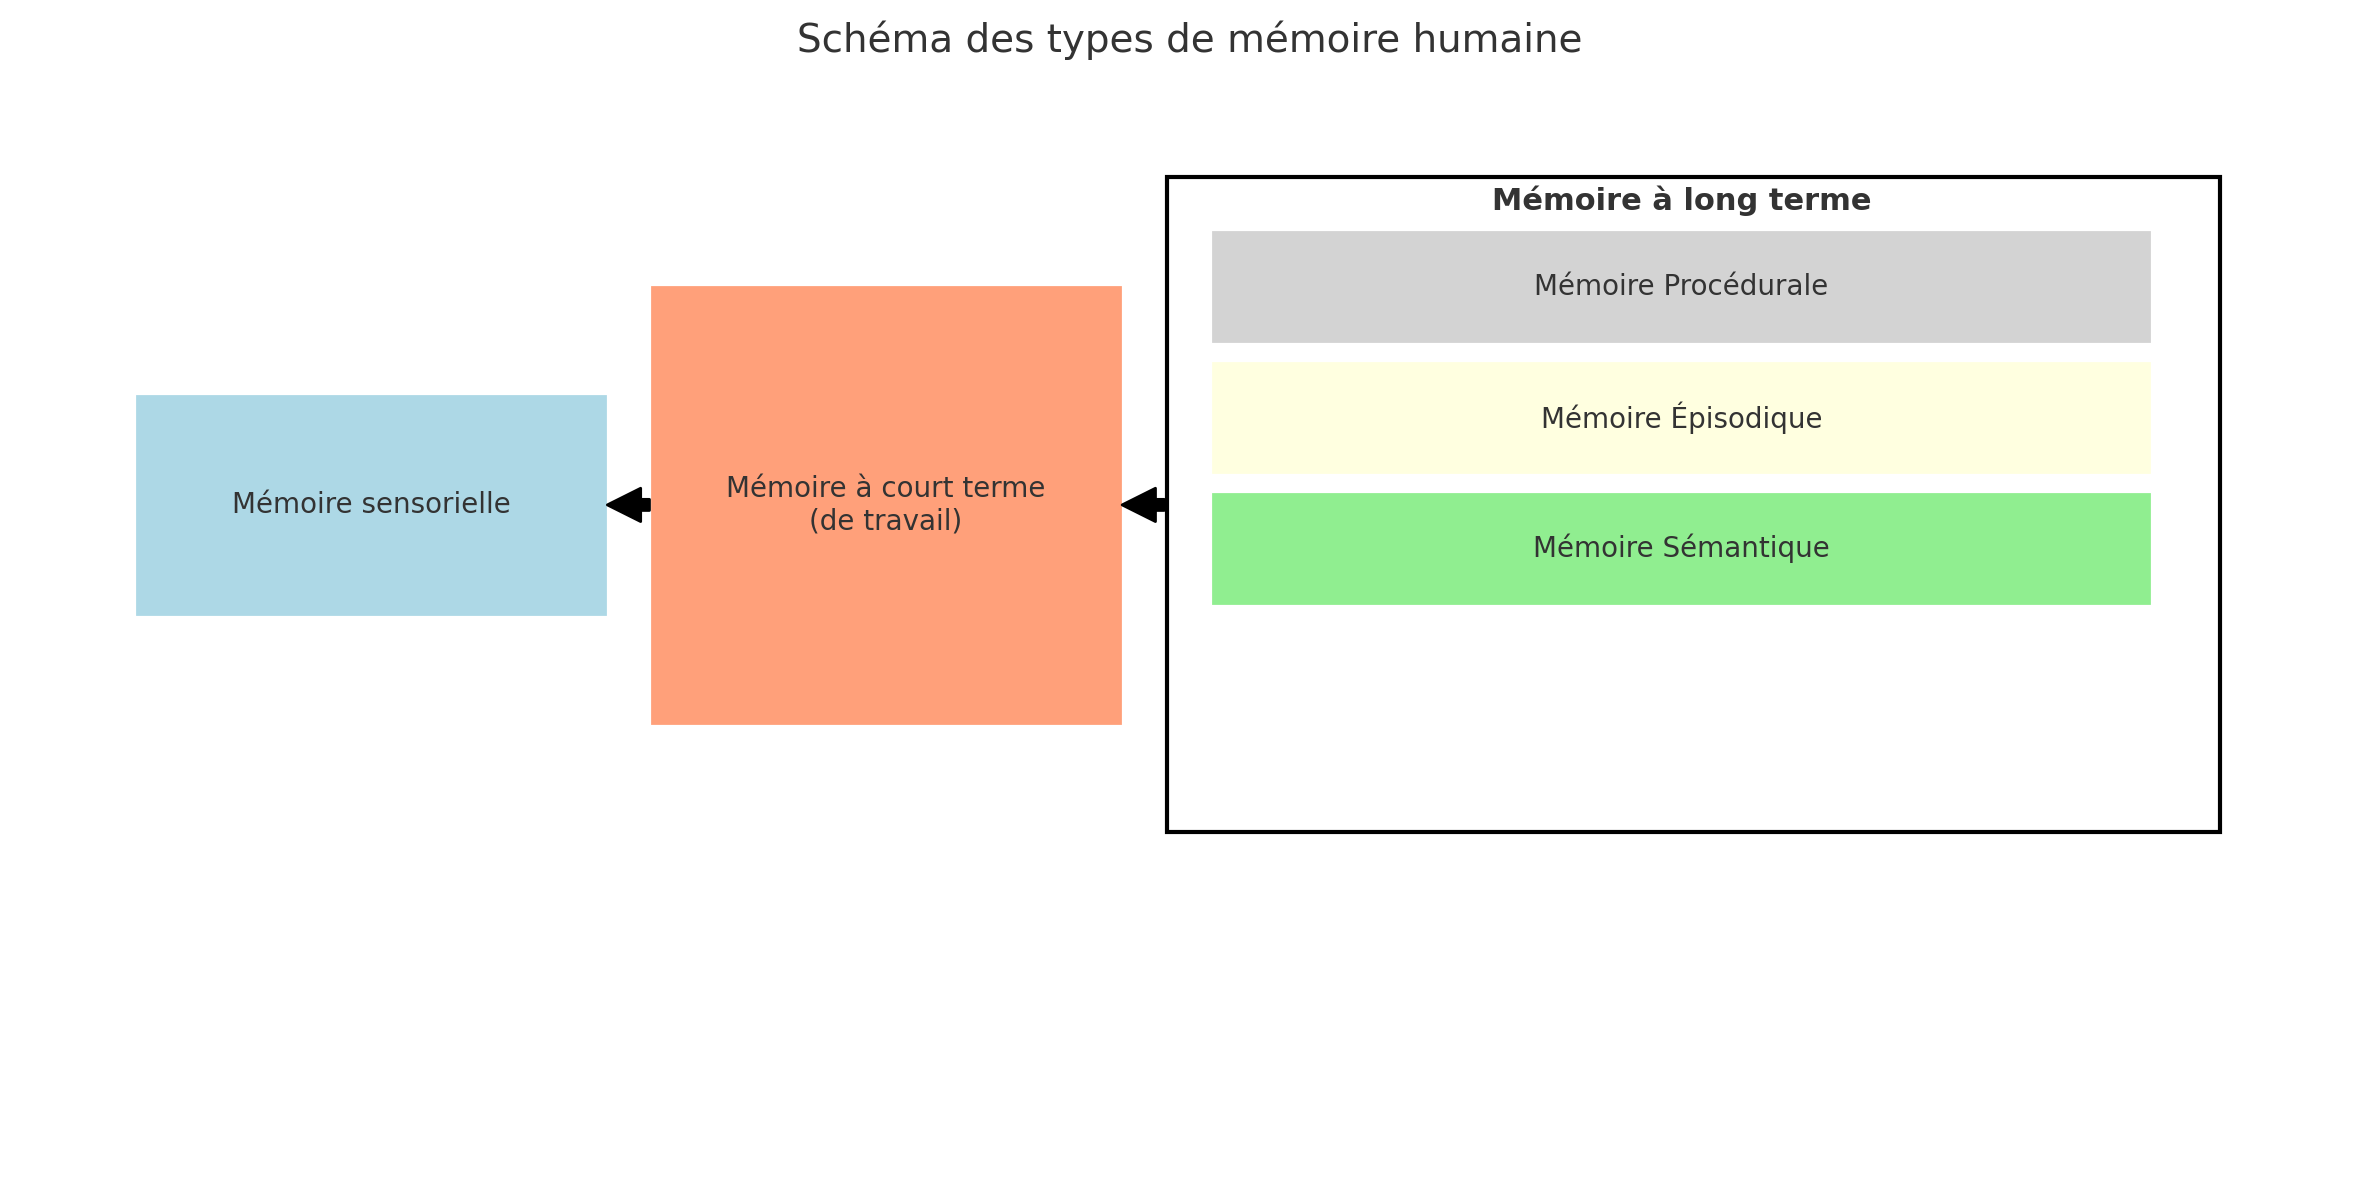
\includegraphics[width=0.7\textwidth]{images/1.1.1.png}
    \caption{Schéma des types de mémoire humaine}
    \label{fig:1.1.1}
\end{figure}

Enfin, je souligne que l’ensemble de ces processus repose sur un phénomène biologique fondamental qu’est la plasticité neuronale, qui désigne la faculté du cerveau à réorganiser ses circuits internes, à créer de nouvelles connexions et à renforcer celles déjà existantes, notamment à la suite d’un apprentissage ou d’une expérience répétée, même si cette capacité tend à diminuer naturellement avec l’âge. 

\vspace{0.5cm}

%1.1.2
\subsection{Facteurs influençant la mémorisation}

Lorsque je cherche à comprendre pourquoi certaines informations s’ancrent solidement dans la mémoire alors que d’autres s’effacent rapidement, je dois prendre en compte un ensemble de facteurs internes et externes qui influencent l’efficacité du processus mnésique à différentes étapes, depuis l’encodage initial jusqu’à la récupération finale.

Je considère d’abord que l’attention constitue la porte d’entrée indispensable à tout processus de mémorisation, puisque seule une information à laquelle j’ai prêté une attention soutenue a une chance d’être traitée en profondeur et intégrée durablement. Lorsque mon attention est concentrée, les réseaux neuronaux impliqués dans l’encodage sont pleinement mobilisés, ce qui facilite la création de traces mnésiques solides. En revanche, si mon attention est dispersée ou superficielle, comme c’est souvent le cas dans les environnements multitâches ou chargés cognitivement, les informations perçues risquent de ne pas dépasser le stade de la mémoire de travail, et seront rapidement perdues.\footnote{Laurence, T. (2012). Fonctionnement et dysfonctionnement de la mémoire. \cite{taconnat}}.

Un autre facteur essentiel réside dans la répétition, car elle permet de renforcer les connexions synaptiques entre les neurones, processus fondamental dans la consolidation mnésique. Je distingue la répétition simple, souvent mécanique, qui se limite à reproduire sans compréhension, et la répétition élaborative, qui suppose une implication cognitive plus forte, en liant les nouvelles informations à celles déjà stockées dans la mémoire à long terme. C’est cette seconde forme qui me semble la plus efficace, car elle repose sur une structuration sémantique du savoir, ce qui facilite non seulement l’encodage mais aussi la récupération ultérieure.\footnote{Pearson. Psychologie \cite{pearson}}.

Je ne peux pas non plus négliger l’influence des émotions sur la mémorisation, car les souvenirs associés à une forte intensité émotionnelle tendent à s’ancrer plus durablement dans ma mémoire. Ce phénomène, que les chercheurs qualifient de mémoire flash, s’explique par l’intervention conjointe de l’amygdale et de l’hippocampe, deux structures cérébrales qui collaborent lorsque l’expérience vécue suscite une réaction émotionnelle marquée. Toutefois, je dois préciser qu’un excès d’émotion, en particulier un stress élevé et prolongé, peut avoir l’effet inverse et altérer le fonctionnement mnésique, notamment en perturbant la plasticité hippocampique à travers l’action du cortisol, hormone libérée lors des situations de stress chronique.\footnote{Françoise S. Maheu \& Sonia J. Lupienn (2003), La mémoire aux prises avec les émotions et le stress \cite{maheulupienn}}.

Enfin, le facteur de l’âge m’amène à considérer que la mémoire évolue tout au long de la vie. Avec le vieillissement, je constate une réduction de la plasticité neuronale et un ralentissement des processus cognitifs, qui affectent principalement la mémoire épisodique. Cependant, je remarque que la mémoire sémantique et la mémoire procédurale sont généralement mieux préservées, ce qui explique pourquoi les connaissances générales et les automatismes acquis persistent souvent malgré l’avancée en âge.\footnote{Francis E. \& Inserm (2019), La Mémoire \cite{inserm}}.

Ces différents éléments, lorsqu’ils sont bien compris, me permettent d’identifier des leviers d’action pour optimiser l’apprentissage et adapter les environnements cognitifs, en particulier grâce aux outils numériques et aux technologies d’intelligence artificielle, qui peuvent soutenir ces processus dans leur complexité.

%1.1.3
\subsection{Processus d’encodage, de stockage et de récupération}

Afin de saisir pleinement le fonctionnement de la mémoire humaine, je m’attarde sur trois étapes fondamentales qui structurent l’édifice mnésique : l’encodage, le stockage et la récupération, chacune jouant un rôle décisif dans la transformation d’une information perçue en souvenir durablement accessible.

\begin{figure}[h]
    \centering
    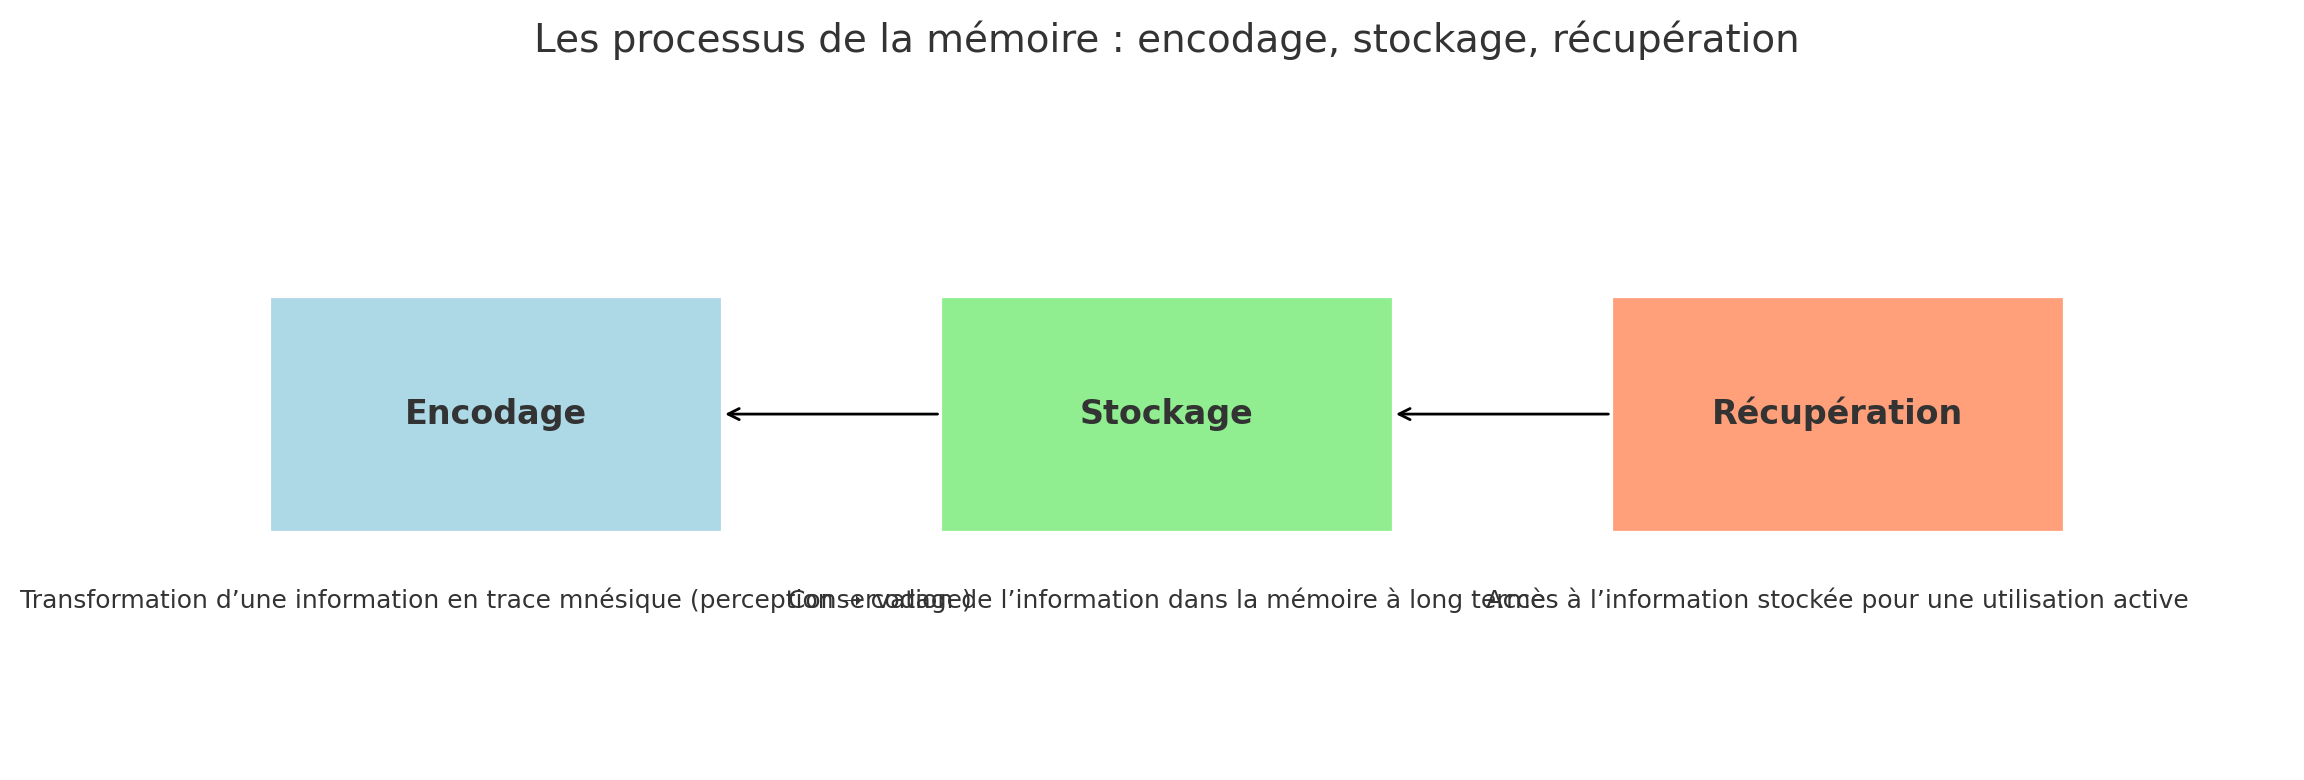
\includegraphics[width=0.7\textwidth]{images/1.1.3.png}
    \caption{Les processus de la mémoire : encodage, stockage, récupération}
    \label{fig:1.1.3}
\end{figure}

Lorsqu’une donnée nouvelle me parvient, je dois tout d’abord la transformer en une trace mentale exploitable, ce qui correspond à la phase d’encodage. Cette opération ne s’effectue pas de manière uniforme ; elle dépend directement du degré d’implication cognitive que je mobilise au moment de l’apprentissage. Plus le traitement de l’information est profond, structuré et sémantique, plus je renforce sa capacité à être durablement intégrée dans mes circuits mnésiques, comme l’ont souligné Craik et Lockhart dans leur modèle des niveaux de traitement, repris et approfondi dans les travaux de David C. (2012)\footnote{David C. (2012), Chronopsychologie et mémoire \cite{clarys}}. Si je me contente d’un traitement superficiel, l’information a peu de chances d’atteindre la mémoire à long terme de manière efficace.

Après cette première transformation cognitive, l’information doit être stockée, c’est-à-dire consolidée au niveau biologique pour pouvoir être maintenue au-delà de la mémoire de travail. Ce processus engage l’hippocampe et les aires corticales, qui participent à deux formes de consolidation distinctes. La première, dite synaptique, se déroule peu de temps après l’apprentissage et renforce les connexions neuronales locales. La seconde, nommée consolidation systémique, s’étale sur une période plus longue et redistribue les informations vers d’autres zones cérébrales, notamment les régions frontales et temporales, comme le décrit Francis Eustache (2019)\footnote{Francis Eustache \& Inserm (2019) La Mémoire \cite{inserm}}. Ce transfert permet la préservation des souvenirs anciens même en cas de dégradation de l’hippocampe, ce qui explique la résilience relative de certains souvenirs personnels ou sémantiques malgré le vieillissement ou certaines atteintes neurologiques.

Lorsque je souhaite accéder à une information précédemment apprise, j’active le processus de récupération, qui consiste à réactiver les réseaux neuronaux associés à la trace mnésique initiale. Cette récupération peut se produire de façon spontanée ou être facilitée par des indices externes tels que l’environnement, les émotions ou des éléments contextuels similaires à ceux présents lors de l’encodage. Toutefois, cette étape dépend étroitement de la qualité des deux phases précédentes. Si l’encodage a été superficiel ou si la consolidation a été entravée, notamment par un stress prolongé qui altère le fonctionnement de l’hippocampe via la sécrétion de cortisol, comme le démontrent les travaux de Maheu et Lupien (2003)\footnote{Françoise S. Maheu \& Sonia J. Lupienn (2003), La mémoire aux prises avec les émotions et le stress \cite{maheulupienn}}, l’accès à l’information peut devenir difficile, voire impossible.

En comprenant la dynamique entre ces trois mécanismes, j’identifie les leviers les plus efficaces pour soutenir les capacités mnésiques, et j’ouvre ainsi la voie à une réflexion sur le rôle que peuvent jouer les technologies intelligentes dans l’optimisation ou la compensation des défaillances de ce cycle cognitif complexe

%1.2
\section{Les troubles affectant la mémorisation}

%1.2.1
\subsection{Vieillissement cognitif et maladies neurodégénératives}

Lorsque je m’interroge sur l’évolution des capacités mnésiques au cours de la vie, je constate que le vieillissement constitue un facteur incontournable, dont les effets peuvent s’observer aussi bien dans le cadre d’un processus cognitif normal que dans celui de pathologies neurodégénératives. Dans le vieillissement dit physiologique, les modifications des fonctions mentales apparaissent de manière progressive et relativement modérée ; elles affectent essentiellement la mémoire épisodique, la vitesse de traitement de l’information et les capacités attentionnelles, sans altérer significativement la mémoire sémantique ni les savoir-faire routiniers, comme le rappellent Eustache (Inserm, 2019)\footnote{Francis Eustache \& Inserm, La mémoire, 2019.  \cite{inserm}}. Ces altérations s’expliquent par une diminution lente mais constante de la plasticité cérébrale, un affaiblissement des transmissions synaptiques, ainsi qu’une atrophie progressive de certaines régions du cerveau, notamment les lobes frontaux et l’hippocampe, qui participent activement aux mécanismes d’encodage et de consolidation des souvenirs.

\begin{figure}[h]
    \centering
    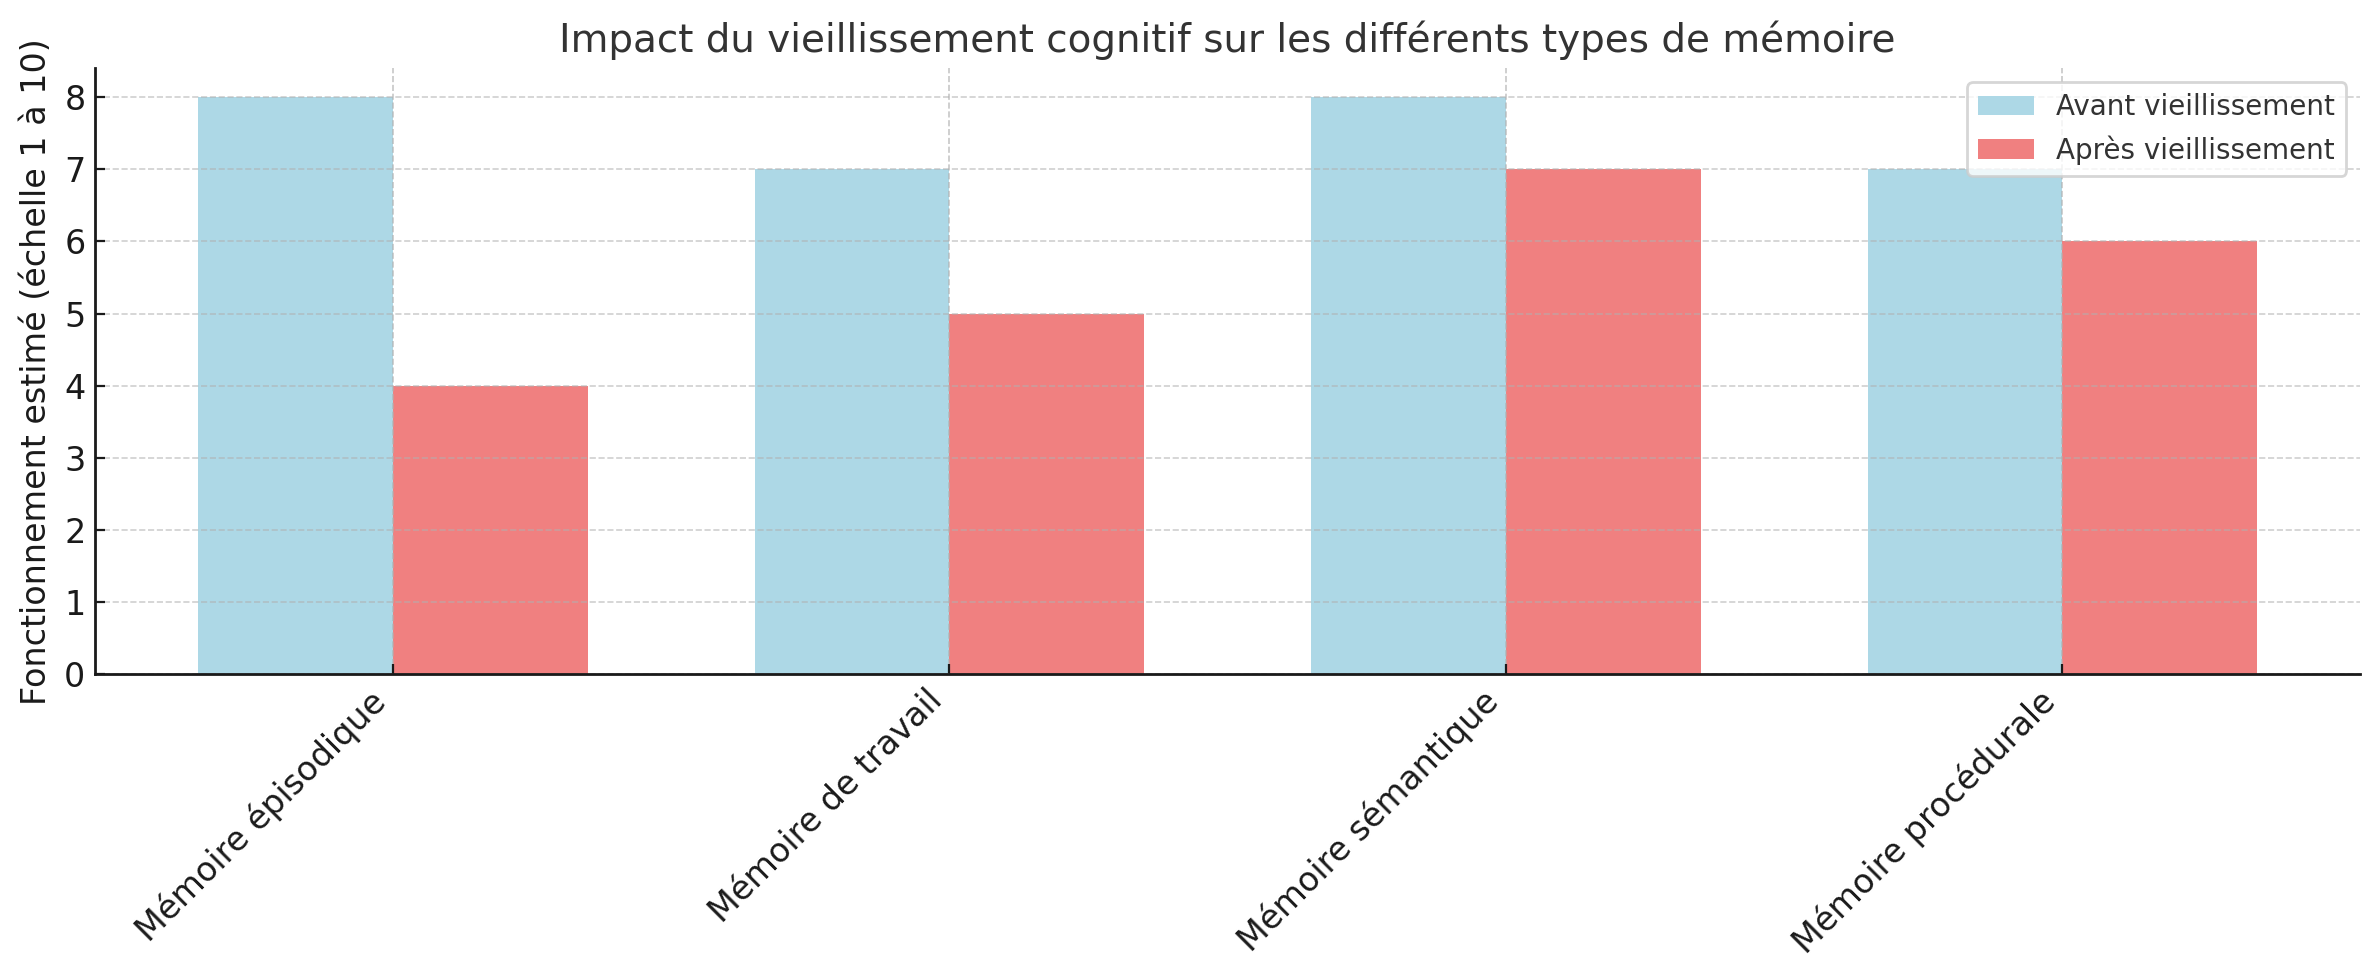
\includegraphics[width=0.7\textwidth]{images/1.2.1.png}
    \caption{Impact du vieillissement cognitif sur les différents types de mémoire}
    \label{fig:1.2.1}
\end{figure}

Cependant, lorsque le vieillissement s’accompagne de pathologies dégénératives, les effets sur la mémoire deviennent plus marqués, plus rapides et plus invalidants. Parmi ces maladies, je retiens tout particulièrement la maladie d’Alzheimer, qui constitue la forme la plus répandue de démence et dont les atteintes précoces concernent principalement la mémoire épisodique. Dès les premiers stades de la maladie, je remarque une difficulté marquée à former de nouveaux souvenirs, phénomène que l’on qualifie d’amnésie antérograde, qui résulte d’une dégénérescence neuronale affectant l’hippocampe et le cortex entorhinal. Au fur et à mesure de la progression de la maladie, les troubles s’étendent à d’autres fonctions cognitives telles que le langage, l’orientation spatio-temporelle et les fonctions exécutives, ce qui conduit inévitablement à une perte d’autonomie, tant sur le plan intellectuel que comportemental. Les mécanismes biologiques en jeu, comme l’accumulation de plaques amyloïdes et la formation de dégénérescences neurofibrillaires, altèrent profondément les réseaux neuronaux, réduisent les capacités de consolidation mnésique, et rompent les circuits de récupération des souvenirs, comme l’a décrit Eustache dans ses travaux récents sur la mémoire cérébrale (Inserm, 2019)\footnote{Francis Eustache \& Inserm, La mémoire, 2019. \cite{inserm}}.

Je note également que d’autres pathologies, comme la maladie de Parkinson, bien que souvent associées aux troubles moteurs, peuvent également entraîner des déficits cognitifs notables. Ces troubles apparaissent dans une proportion significative de cas et concernent principalement la mémoire de travail et la mémoire procédurale. La réduction de la dopamine, neurotransmetteur essentiel au bon fonctionnement des circuits fronto-striataux, semble jouer un rôle central dans cette détérioration progressive des fonctions mnésiques, comme le montrent les recherches menées par Corvol (Inserm (2022))\footnote{Jean-Christophe Corvol \& Inserm, La maladie de Parkinson, 2022. \cite{inserm2}}..

En explorant les effets du vieillissement cognitif et des pathologies neurodégénératives sur la mémoire, je comprends que la perte de souvenirs n’est pas uniquement une question de quantité d’information oubliée, mais aussi un effacement progressif de la capacité à organiser, interpréter et utiliser ces souvenirs dans la vie quotidienne. Cela m’amène à envisager des pistes d’intervention qui, grâce aux technologies d’intelligence artificielle, pourraient à la fois compenser ces déficits, stimuler les fonctions résiduelles et prolonger l’autonomie cognitive des personnes concernées.

%1.2.2
\subsection{Troubles de l’attention et de l’apprentissage (TDAH, dyslexie)}

Lorsque je m’intéresse aux troubles qui perturbent les mécanismes mnésiques dès l’enfance ou à l’âge adulte, je ne peux ignorer l’impact majeur que représentent les troubles de l’attention et de l’apprentissage, en particulier le trouble du déficit de l’attention avec ou sans hyperactivité (TDAH) et la dyslexie. Ces deux conditions, bien qu’hétérogènes dans leurs manifestations, ont en commun de compromettre l’efficience de l’encodage initial, ce qui entraîne des répercussions sur le stockage et la récupération des informations dans la mémoire.

\begin{figure}[h]
    \centering
    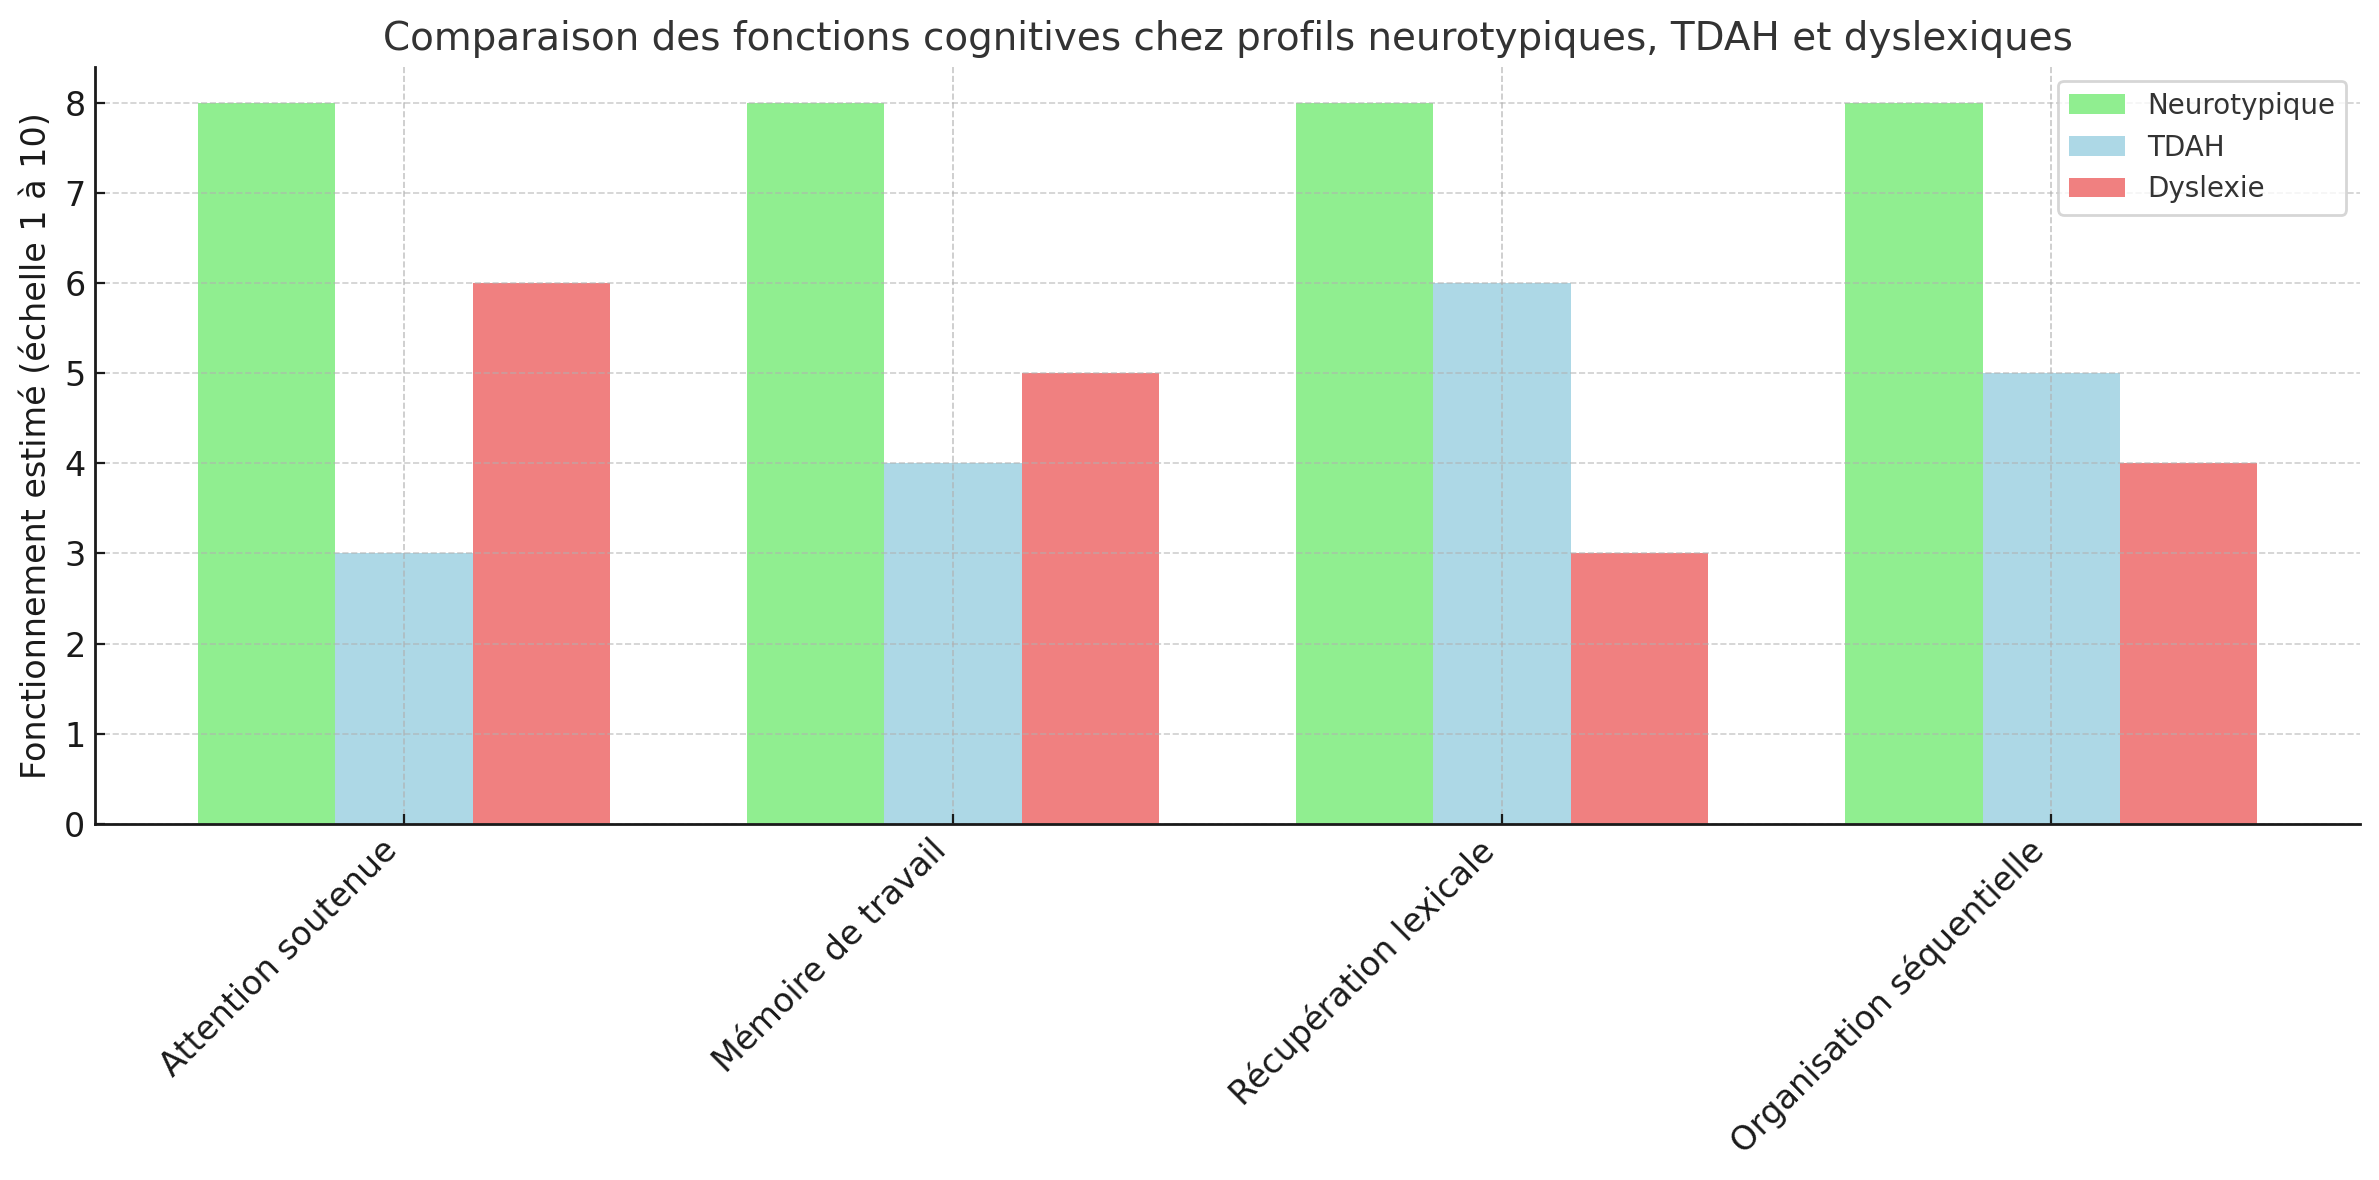
\includegraphics[width=0.7\textwidth]{images/1.2.2.png}
    \caption{Comparaison des fonctions cognitives chez profils neurotypiques, TDAH et dyslexiques}
    \label{fig:1.2.2}
\end{figure}

Dans le cas du TDAH, je constate que l’incapacité à maintenir une attention soutenue constitue l’un des premiers obstacles à une mémorisation efficace. Le traitement de l’information reste superficiel lorsque la concentration est instable, ce qui compromet la formation de traces mnésiques durables. Cette faiblesse attentionnelle empêche les informations de franchir le seuil de la mémoire de travail et d’être transférées de manière optimale vers la mémoire à long terme\footnote{Inserm 2022. C’est quoi le TDAH ? \cite{inserm3}}.. Les recherches sur le TDAH montrent clairement que ce trouble affecte la gestion cognitive des tâches séquentielles et la planification mentale, deux compétences essentielles à l’organisation des souvenirs dans le temps. De plus, les données recueillies par Alice (2023)\footnote{Alice 2023. TDAH et mémoire de travail. \cite{minicoachtdah}}. soulignent que les enfants et les adultes atteints de TDAH présentent fréquemment des déficits dans la mémoire de travail verbale, ce qui les empêche de manipuler mentalement des informations sur de courtes périodes, un processus pourtant fondamental dans l’apprentissage et la résolution de problèmes.

La dyslexie, de son côté, affecte la capacité à décoder, reconnaître et automatiser les représentations écrites du langage, ce qui complique fortement l’encodage phonologique et visuel des mots. Je remarque que cette difficulté ralentit l’accès au sens des textes, ce qui nécessite une mobilisation accrue de ressources cognitives pour chaque tâche de lecture, limitant ainsi la disponibilité cognitive pour l’encodage en mémoire. Comme l’indiquent Lexidys (2020)\footnote{Lexidys. 2020, Dyslexie développementale : dossier médical et actu. \cite{lexidys}}, ce trouble perturbe l’élaboration de représentations mentales stables, nécessaires à la mémorisation à long terme, et complique la généralisation des apprentissages. Les personnes dyslexiques doivent alors consacrer une énergie mentale plus importante à la lecture, ce qui limite leur capacité à traiter les informations en profondeur et à en assurer la consolidation.

J’observe également que ces troubles ne se résument pas à des difficultés cognitives isolées, car ils s’accompagnent souvent d’effets émotionnels négatifs tels que la frustration, le découragement ou une faible estime de soi. Ces facteurs émotionnels, en créant un climat d’anxiété ou de stress, peuvent accentuer les déficiences mnésiques déjà présentes, en affectant notamment la récupération des souvenirs ou la concentration lors de l’apprentissage. Ces observations me conduisent à considérer que les stratégies d’accompagnement ne doivent pas se limiter à des ajustements pédagogiques, mais qu’elles doivent également prendre en compte la dimension affective de l’apprentissage.

Dans cette optique, je considère que les outils numériques, en particulier ceux mobilisant l’intelligence artificielle, offrent un potentiel prometteur pour répondre aux besoins spécifiques de ces profils cognitifs. Les systèmes adaptatifs, capables de détecter en temps réel les difficultés d’un apprenant et d’ajuster dynamiquement les contenus proposés, représentent une piste concrète pour favoriser une mémorisation plus efficace chez les personnes atteintes de TDAH ou de dyslexie.

%1.2.3
\subsection{Surcharge cognitive et oubli informationnel}

Lorsque j’analyse les raisons pour lesquelles certaines informations ne parviennent pas à s’ancrer durablement dans la mémoire, je dois accorder une attention particulière à la notion de surcharge cognitive, phénomène central dans les environnements d’apprentissage modernes. Je constate que la mémoire de travail, par nature limitée dans sa capacité, ne peut traiter qu’un nombre restreint d’éléments simultanément. Lorsque cette limite est dépassée, les nouvelles informations ne peuvent plus être encodées correctement et risquent d’être perdues, soit parce qu’elles n’ont pas été traitées suffisamment en profondeur, soit parce qu’elles ont été immédiatement remplacées par d’autres, dans un flux ininterrompu d’entrées mentales.

\begin{figure}[h]
    \centering
    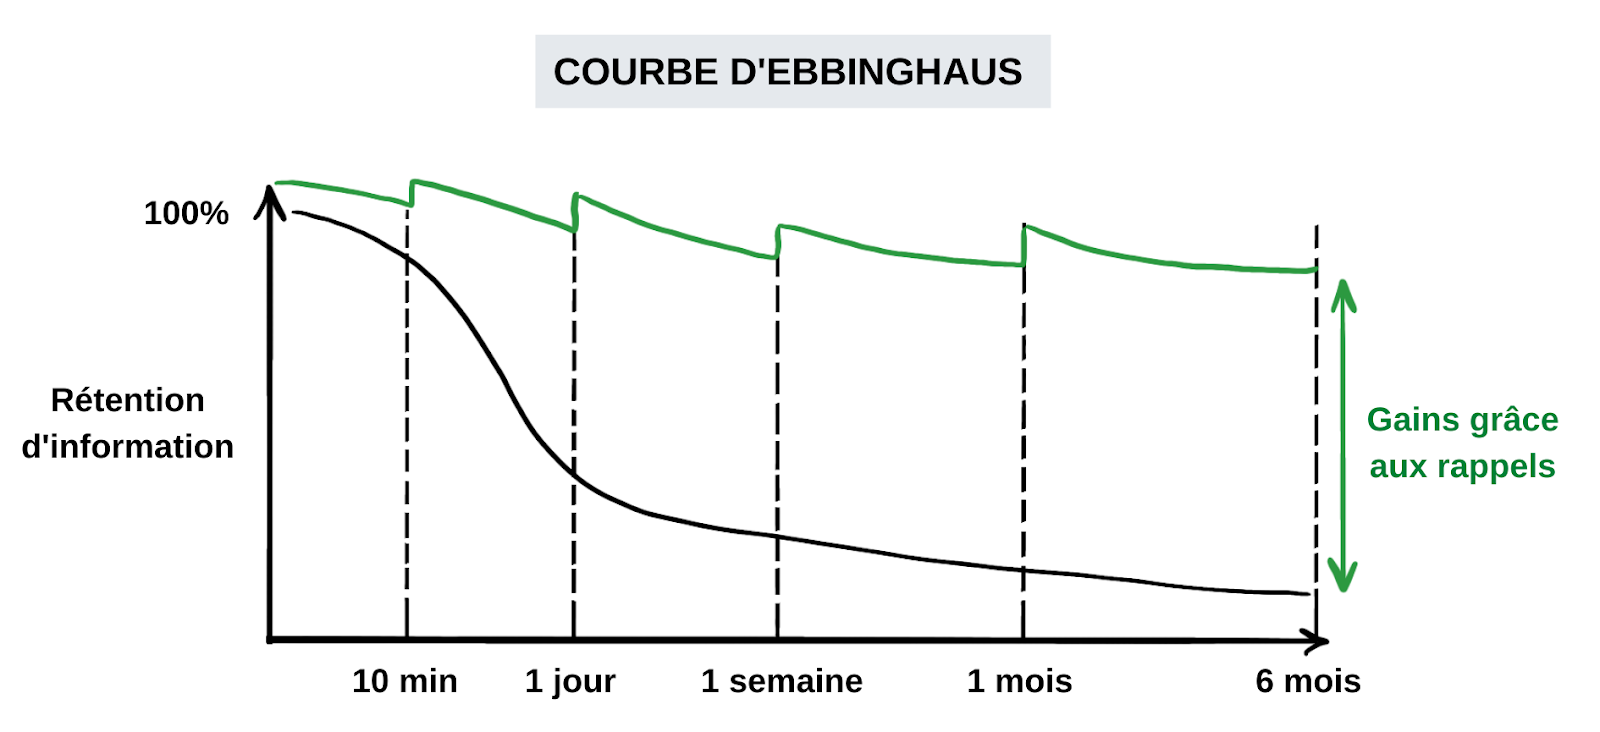
\includegraphics[width=0.7\textwidth]{images/1.2.3.png}
    \caption{Effet de la surcharge cognitive sur la performance}
    \label{fig:1.2.3}
\end{figure}

Ce constat a été théorisé dès les travaux de Sweller dans les années 1980, et plus récemment repris par l’Académie d’Aix-Marseille (2022)\footnote{John Sweller, Académie d'AIX-marseille, 2022. La Théorie de la charge cognitive \cite{sweller}}, sous le nom de théorie de la charge cognitive, selon laquelle je distingue plusieurs formes de surcharge. La charge intrinsèque correspond à la complexité inhérente d’une tâche, comme résoudre un problème abstrait, qui sollicite fortement mes capacités mentales. La charge extrinsèque provient quant à elle d’éléments non essentiels, mal structurés ou redondants, qui mobilisent inutilement mes ressources cognitives et perturbent l’apprentissage. Enfin, la charge germane représente la part bénéfique de l’activité mentale, celle qui contribue directement à la construction de nouveaux schémas de pensée et à l’intégration des connaissances dans la mémoire à long terme.

Lorsque cette balance entre les différents types de charge n’est pas maîtrisée, je me retrouve face à un phénomène d’oubli informationnel. Les informations peuvent ne pas être encodées de manière efficace ou ne pas bénéficier d’une consolidation suffisante, faute d’un traitement approprié ou d’un contexte d’apprentissage favorable. Ce type d’oubli ne traduit donc pas nécessairement un déficit biologique, mais souvent un environnement d’apprentissage mal optimisé, saturé de stimulations et peu propice à la structuration cognitive.

Dans les contextes éducatifs contemporains, je remarque que cette surcharge est amplifiée par la surabondance d’informations diffusées simultanément par divers canaux (textes, images, vidéos, sons), qui sollicitent de manière excessive la mémoire de travail. Cette sollicitation entraîne une fragmentation de l’attention, nuit à la sélection des informations pertinentes et compromet l’encodage profond, comme le rappelle Sweller dans sa modélisation du traitement cognitif.\footnote{John Sweller, La théorie de la charge cognitive. \cite{sweller2}}.

Pour faire face à cette situation, je m’intéresse aux stratégies pédagogiques capables de réduire cette surcharge, comme la structuration progressive des contenus, la présentation espacée des informations ou encore l’utilisation d’éléments visuels qui facilitent l’organisation mentale. Toutefois, je considère que ces méthodes, bien que précieuses, trouvent leurs limites lorsqu’il s’agit d’ajuster finement le contenu à chaque profil cognitif.

C’est dans ce cadre que l’intelligence artificielle représente, selon moi, une opportunité particulièrement pertinente. En intégrant des systèmes capables d’analyser en temps réel le niveau de saturation cognitive d’un utilisateur, je peux imaginer des outils qui adaptent dynamiquement le rythme d’apprentissage, sélectionnent les informations les plus pertinentes et suggèrent des temps de pause ou de répétition adaptés. Ces dispositifs, en s’appuyant sur la répétition espacée ou la détection des difficultés, offrent des perspectives concrètes pour prévenir la surcharge cognitive et limiter l’oubli informationnel, en optimisant la gestion des ressources mentales disponibles à chaque instant.

%1.3
\section{Les stratégies d’aide à la mémorisation}

%1.3.1
\subsection{Méthodes traditionnelles (mnémoniques, répétition espacée)}

Lorsque je cherche à améliorer ma capacité de mémorisation, je me tourne d’abord vers des méthodes traditionnelles qui ont traversé les siècles et dont l’efficacité a été reconnue bien avant l’avènement des outils numériques ou des technologies intelligentes. Ces stratégies, fondées sur l’optimisation des processus d’encodage et de récupération, s’appuient sur des principes cognitifs simples mais puissants, tels que l’association mentale, la visualisation structurée ou la régularité des révisions.

\begin{figure}[h]
    \centering
    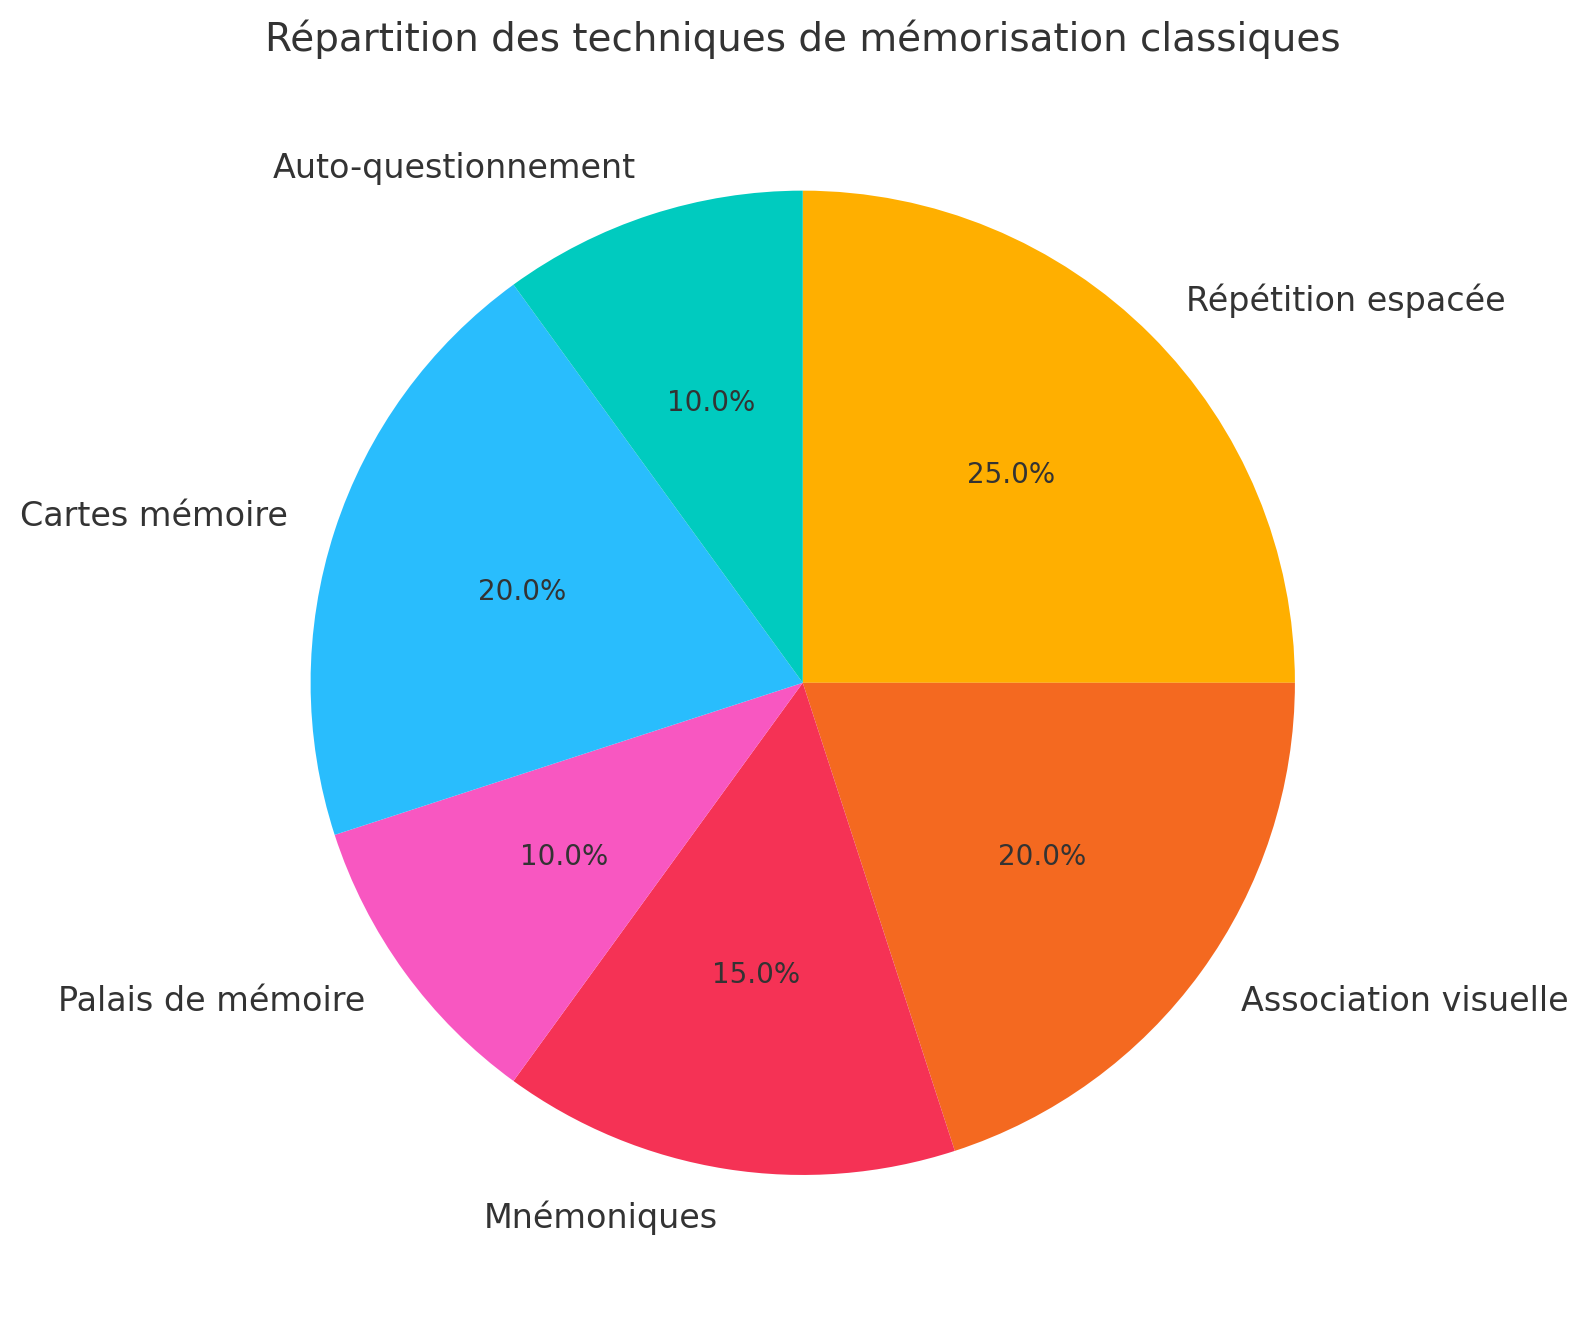
\includegraphics[width=0.7\textwidth]{images/1.3.1.png}
    \caption{Répartition des techniques de mémorisation classiques}
    \label{fig:1.3.1}
\end{figure}

Parmi les techniques les plus anciennes que j’ai expérimentées ou étudiées, je retiens les méthodes mnémoniques, qui visent à faciliter la rétention d’informations en les associant à des éléments familiers, concrets ou visuellement marquants. En construisant des images mentales ou en créant des phrases-clés à partir d’acronymes, je parviens à structurer l’information d’une manière qui facilite son accès ultérieur. J’accorde une attention particulière à la méthode des lieux, aussi appelée méthode du palais mental, dont les origines remontent à l’Antiquité et qui consiste à associer des informations à des lieux bien connus dans un ordre précis, ce qui permet de naviguer mentalement dans un espace fictif pour retrouver les éléments mémorisés. Cette technique, encore largement utilisée dans les concours de mémoire, est reconnue pour son efficacité par les chercheurs en psychologie cognitive, comme le rappelle un article de Psychomédia (2017) consacré aux loci.\footnote{Psychomédia. 2017. La méthode des loci pour améliorer la mémorisation \cite{psychomédia}}.

Au-delà des associations mentales, je m’appuie également sur la répétition espacée, méthode dont les fondements ont été posés par Hermann Ebbinghaus à la fin du XIXe siècle, lorsqu’il a démontré que la mémoire humaine suit une courbe d’oubli rapide si l’information n’est pas consolidée par des rappels réguliers. En espaçant volontairement mes révisions selon des intervalles croissants, je renforce le processus de consolidation mnésique et je permets aux traces neuronales de se stabiliser durablement dans la mémoire à long terme. L’Académie de Nantes (2021)\footnote{Académie de Nantes. La courbe de l'oubli d'Ebbinghaus. \cite{ebbinghaus}} a d’ailleurs repris cette notion en expliquant comment cette stratégie peut réduire de manière significative l’oubli naturel lié au temps.

Je note que cette méthode, bien qu’efficace, requiert une certaine rigueur dans son application, car elle suppose de respecter des délais précis entre chaque rappel, ce qui peut parfois représenter une contrainte logistique ou organisationnelle pour l’apprenant. De plus, comme l’indique la plateforme Pamplemousse (2022)\footnote{Pamplemousse , La méthode de la répétition espacée pour apprendre ses cours. \cite{pamplemousse}}, la répétition espacée ne produit ses effets que si elle s’inscrit dans une démarche active, où je m’efforce non seulement de relire, mais aussi de tester ma capacité à rappeler l’information, ce qui renforce la consolidation par la récupération.

Même si ces approches ne nécessitent aucune technologie, je les considère comme des fondations solides sur lesquelles peuvent se greffer des outils modernes. Leur simplicité, leur accessibilité et leur universalité les rendent pertinentes dans de nombreux contextes d’apprentissage, y compris pour des personnes présentant des troubles cognitifs, dès lors qu’elles sont bien encadrées. Elles constituent pour moi une base méthodologique incontournable, que les technologies d’intelligence artificielle peuvent enrichir, mais non remplacer.

%1.3.2
\subsection{Utilisation des technologies numériques actuelles}

Lorsque je réfléchis à l’évolution des méthodes de mémorisation dans les sociétés contemporaines, je constate que les technologies numériques occupent une place croissante dans les dispositifs d’aide cognitive, en offrant des solutions interactives, adaptables et souvent motivantes pour renforcer l’apprentissage et la rétention de l’information. Ces outils, bien qu’ils reposent sur les mêmes principes fondamentaux que les méthodes traditionnelles, les dépassent par leur capacité à s’adapter dynamiquement aux besoins spécifiques de chaque utilisateur, en exploitant la puissance du traitement algorithmique et la flexibilité des interfaces numériques.

\begin{figure}[h]
    \centering
    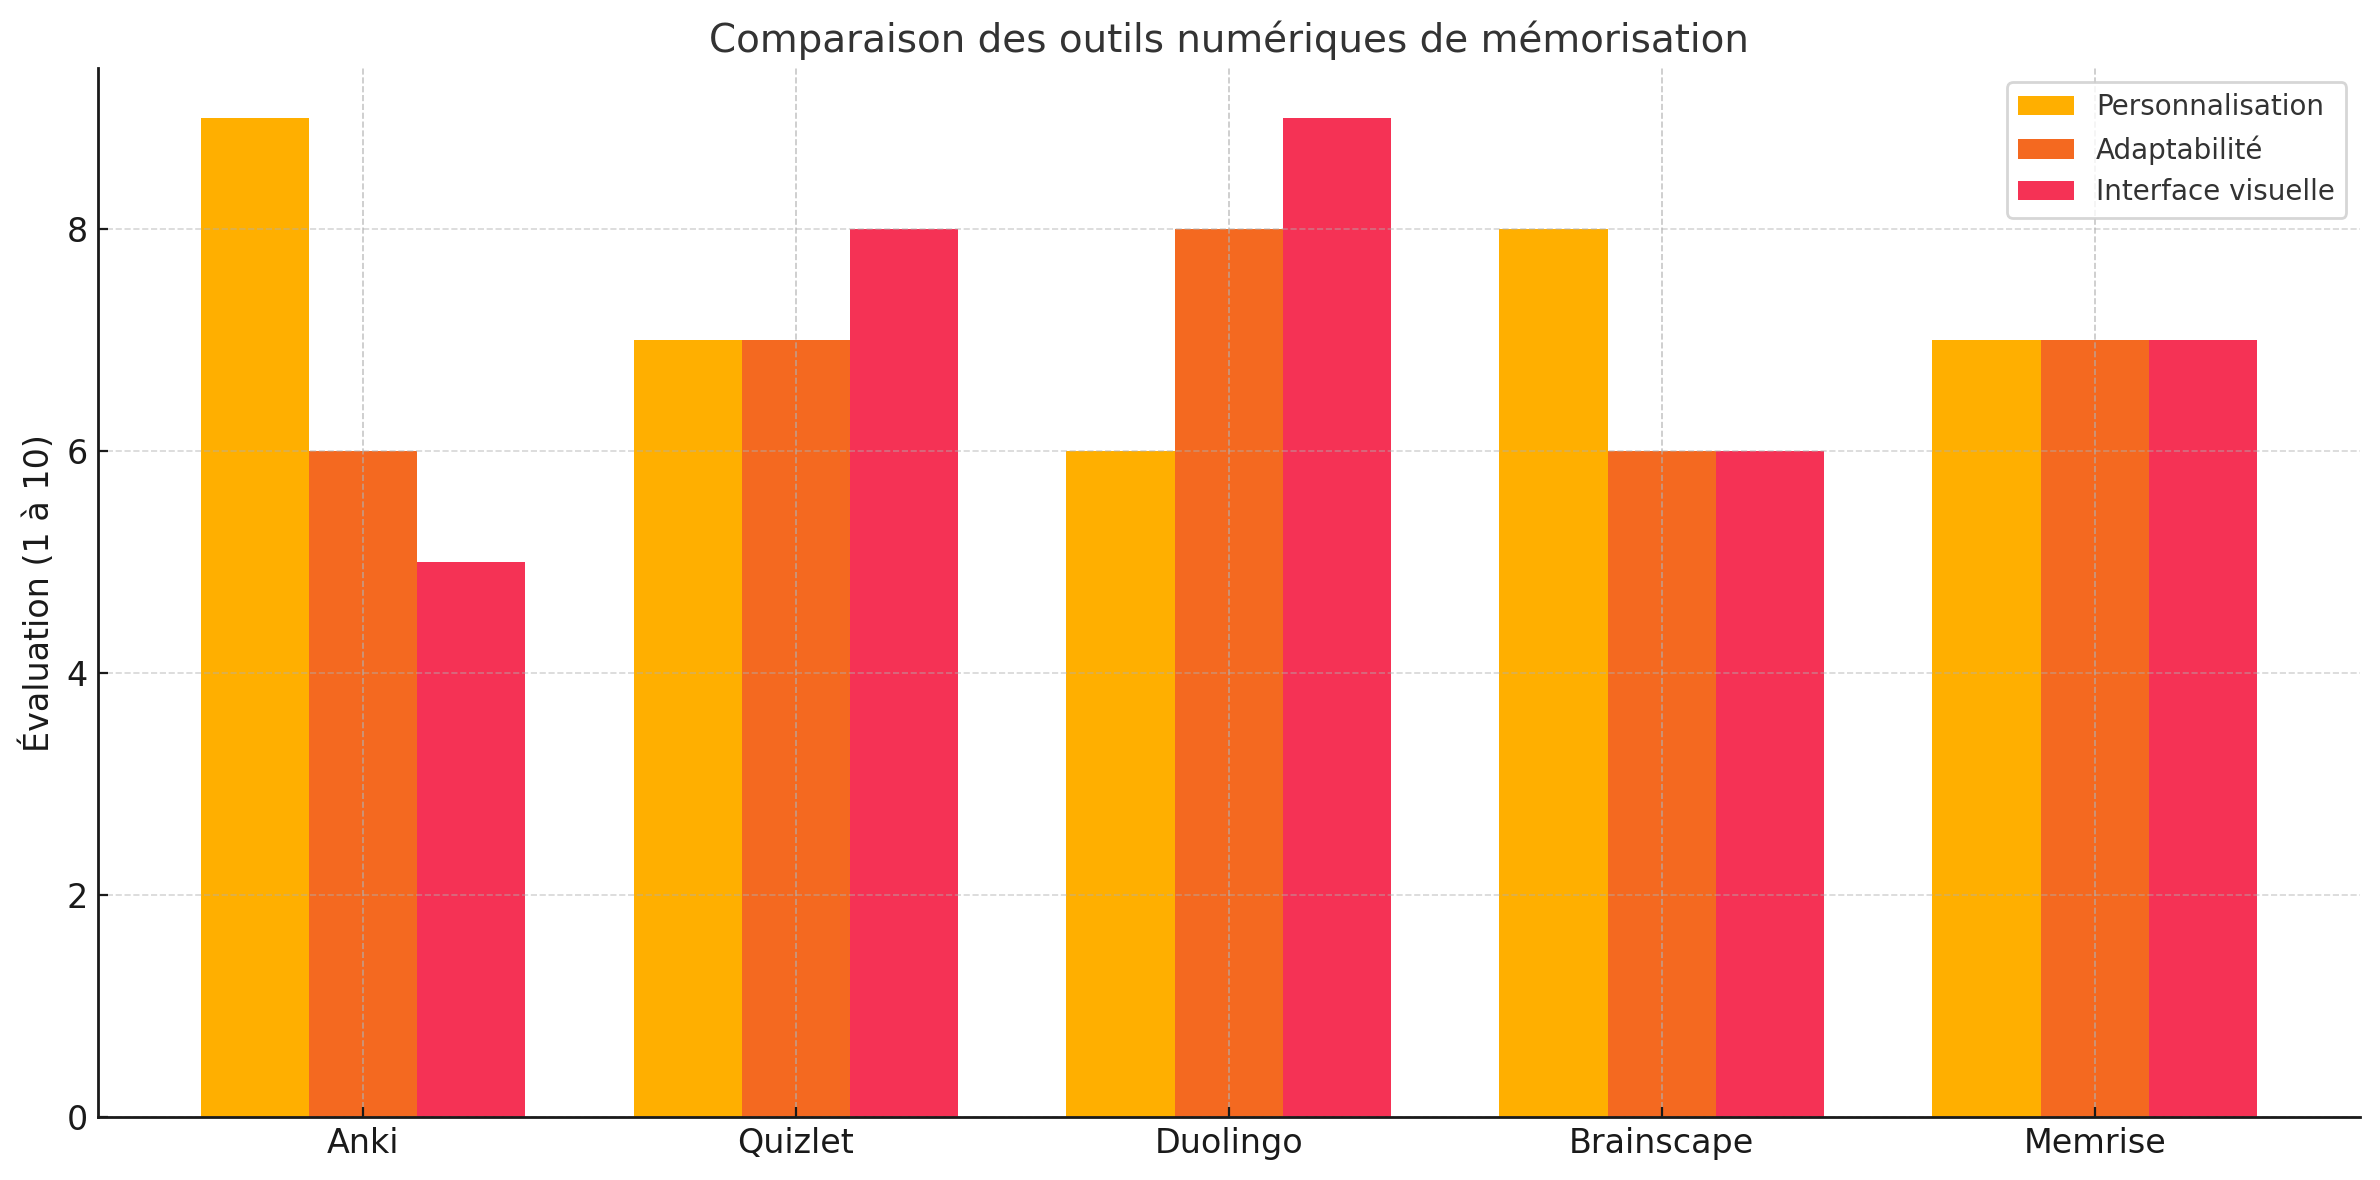
\includegraphics[width=0.7\textwidth]{images/1.3.2.png}
    \caption{Comparaison des outils numériques de mémorisation}
    \label{fig:1.3.2}
\end{figure}

Parmi les applications que j’ai utilisées ou analysées, j’observe que des plateformes comme Anki, Memrise ou Quizlet exploitent efficacement les mécanismes de la répétition espacée, en intégrant des algorithmes capables de calculer les intervalles optimaux entre deux rappels en fonction de ma performance et de mes erreurs précédentes. Grâce à ce suivi individualisé, je peux renforcer mes souvenirs de manière ciblée, sans avoir à organiser manuellement mes révisions. Ces outils, en associant un contenu structuré à des interfaces ludiques, me permettent de maintenir un engagement régulier dans l’apprentissage, ce qui constitue une réponse concrète au manque de motivation souvent observé dans les approches purement disciplinaires. Le Conseil supérieur de l’éducation du Québec (2020)\footnote{CSE Quebec 2020, L’intelligence artificielle en éducation \cite{hypotheses}}, dans son rapport sur l’intelligence artificielle en éducation, met en avant l’efficacité de ces plateformes pour améliorer la mémorisation par des stratégies pédagogiques automatisées mais personnalisées.

Au-delà de ces applications spécialisées, je m’appuie aussi sur des gestionnaires de tâches et de notes numériques, comme Google Keep, Notion ou Evernote, qui me permettent de structurer l’information de manière visuelle et hiérarchique. Ces outils, en facilitant l’organisation des idées et des rappels, réduisent ma charge cognitive extrinsèque, en externalisant les contraintes de planification et de suivi. Je peux ainsi concentrer mon attention sur le contenu à mémoriser, plutôt que sur les aspects logistiques de l’apprentissage. En structurant mes connaissances sous forme de cartes mentales, de tableaux dynamiques ou de calendriers intelligents, je crée un environnement propice à l’encodage en profondeur, et j’améliore l’accessibilité de mes souvenirs.

Je remarque également que ces technologies tirent parti de la multimodalité pour enrichir l’expérience cognitive. En combinant des supports visuels, sonores, textuels et interactifs, elles sollicitent plusieurs canaux sensoriels simultanément, ce qui renforce la consolidation mnésique en créant des représentations mentales plus riches et plus robustes. Dans le domaine de l’apprentissage linguistique ou scientifique, cette approche intégrée me permet d’associer les sons, les images et les concepts de manière cohérente, ce qui favorise la mémorisation de structures complexes. Le CSE Québec (2020)\footnote{CSE Quebec 2020, L’intelligence artificielle en éducation \cite{hypotheses}} souligne que cette capacité à moduler l'information selon différents formats constitue l’un des atouts majeurs des environnements numériques d’apprentissage.

Enfin, je m’intéresse aux technologies émergentes comme la réalité virtuelle ou augmentée, qui plongent l’apprenant dans des environnements immersifs et simulés. Ces expériences, en augmentant l’engagement émotionnel et sensoriel, créent des contextes d’apprentissage plus marquants, où les connaissances sont mieux intégrées grâce à une implication active. Dans le domaine médical ou technique, ces outils permettent de répéter des gestes ou des procédures en situation virtuelle, ce qui favorise la consolidation procédurale tout en réduisant les risques d’erreur. Le rapport de Startum (2023)\footnote{Startum. 2023. Apprentissage immersif : la réalité virtuelle et la réalité augmentée dans l'éducation. \cite{startum}} sur les usages éducatifs de la réalité virtuelle met en évidence l’impact positif de ces technologies sur la rétention des savoirs pratiques, notamment chez les apprenants adultes.

En articulant ces outils à mes besoins cognitifs et en les intégrant de manière réfléchie à mon parcours d’apprentissage, je peux optimiser mes performances mnésiques tout en développant une autonomie renforcée. Toutefois, cette évolution suppose aussi que je sois accompagné dans leur utilisation, afin de ne pas en faire un simple substitut, mais un véritable amplificateur de mes capacités naturelles.

%1.3.3
\subsection{Limites des approches classiques}

Lorsque j’évalue l’efficacité des outils que j’utilise pour soutenir ma mémoire, qu’ils soient traditionnels ou numériques, je me rends compte qu’aucune méthode, aussi bien pensée soit-elle, ne peut se prétendre universelle ni totalement infaillible. Malgré leur utilité indéniable dans l’amélioration de la mémorisation, ces dispositifs présentent des limites qu’il m’importe de considérer si je souhaite adopter une démarche critique et équilibrée face aux solutions disponibles.

\begin{figure}[h]
    \centering
    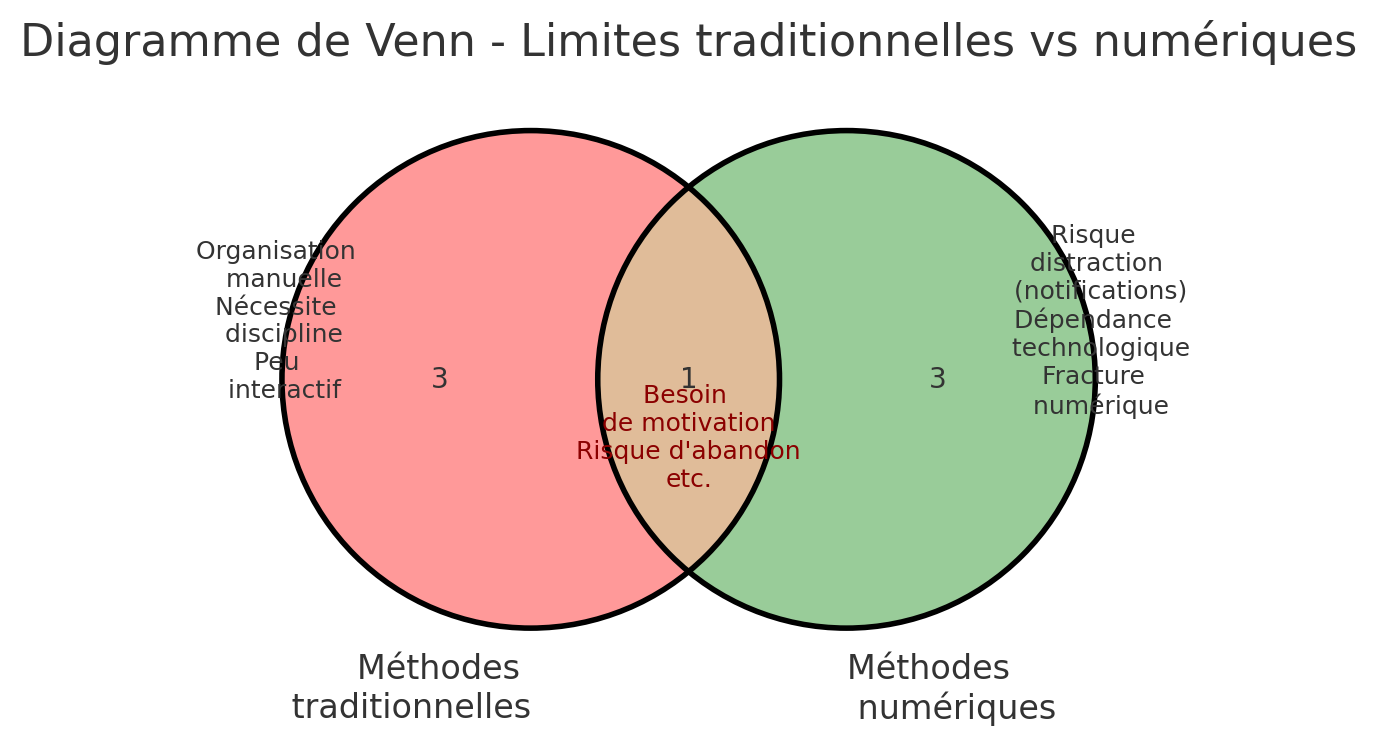
\includegraphics[width=0.7\textwidth]{images/1.3.3.png}
    \caption{Limites des approches traditionnelles vs IA cognitive}
    \label{fig:1.3.3}
\end{figure}

En ce qui concerne les méthodes traditionnelles, je reconnais qu’elles requièrent une implication personnelle constante et une discipline rigoureuse. La répétition espacée, par exemple, bien qu’efficace sur le plan théorique, exige une organisation temporelle précise et une régularité d’application qui peuvent devenir contraignantes dans un quotidien chargé. Si je ne respecte pas les intervalles recommandés, l’effet bénéfique de cette méthode diminue, et l’information risque de s’éroder malgré mes efforts. De plus, les techniques mnémoniques, aussi puissantes soient-elles, ne conviennent pas à tous les types de contenus. Lorsque les données à mémoriser sont abstraites, complexes ou non verbales, ces stratégies perdent de leur efficacité, comme le rappellent les chercheurs cités dans les travaux de Psychomédia (2017)\footnote{Psychomédia. 2017. La méthode des loci pour améliorer la mémorisation \cite{psychomédia}}.

Du côté des outils numériques, je constate que leur efficacité repose largement sur la qualité de l’implémentation algorithmique et sur leur adaptation réelle à mes besoins. Certains dispositifs, bien qu’intelligents sur le papier, se révèlent trop génériques dans leur approche et n’offrent pas un niveau de personnalisation suffisant pour répondre à mes spécificités cognitives. D’autres, au contraire, sollicitent une quantité excessive d’informations ou multiplient les notifications, ce qui peut paradoxalement contribuer à une surcharge cognitive, en détournant mon attention plutôt qu’en la canalisant. Comme le souligne le rapport du CSE Québec (2020)\footnote{CSE Quebec 2020, L’intelligence artificielle en éducation \cite{hypotheses}}, l’usage intensif des technologies numériques en éducation peut, dans certains cas, engendrer une fragmentation de l’attention, une perte de repères dans la hiérarchisation des contenus et un sentiment de dépendance vis-à-vis des supports externes.

Je remarque également que ces outils numériques, s’ils ne sont pas encadrés par une réflexion pédagogique claire, risquent de me placer dans une posture passive où l’automatisation remplace l’effort cognitif. Dans ce cas, je tends à déléguer à la machine ce que je pourrais exercer moi-même, ce qui peut nuire au développement de mes propres stratégies métacognitives. Cette dépendance technologique, que certains auteurs qualifient de délégation cognitive, m’amène à repenser la place des outils dans mon apprentissage, non comme des substituts à mes fonctions mentales, mais comme des extensions temporaires, dont l’usage doit rester conscient, contrôlé et évalué.

Enfin, je n’ignore pas les inégalités d’accès à ces outils, qu’ils soient matériels ou culturels. Certaines personnes, en raison de leurs conditions sociales, économiques ou éducatives, n’ont pas la possibilité d’exploiter ces ressources, ce qui creuse un fossé numérique dans les capacités d’apprentissage et de mémorisation. Le rapport de Talan (2024) met en lumière cette fracture technologique et pédagogique, qui risque d’amplifier les écarts déjà existants entre les individus en matière d’accès au savoir et d’autonomie cognitive.\footnote{Talan. 2024. L'impact des inégalités d'accès aux technologies sur l'éducation \cite{talan}}.

Ainsi, je considère que si les outils traditionnels et numériques offrent un potentiel réel pour soutenir mes efforts mnésiques, leur efficacité dépend étroitement du contexte d’utilisation, de l’accompagnement dont je bénéficie et de ma capacité à en faire un usage éclairé et critique.

%2
\chapter{L’intelligence artificielle au service de la mémoire}

%2.1
\section{Comprendre le fonctionnement de l’intelligence artificielle}

%2.1.1
\subsection{Définition et fonctionnement de l’intelligence artificielle}

Lorsque je cherche à définir ce que recouvre précisément le terme d’intelligence artificielle, je m’appuie sur une approche à la fois technique et conceptuelle, car ce champ, bien qu’omniprésent dans les discours contemporains, demeure complexe dans ses contours et ses implications. L’intelligence artificielle, que je désigne par le sigle IA, correspond à un ensemble de techniques informatiques qui visent à reproduire certaines fonctions cognitives humaines, comme l’apprentissage, le raisonnement, la reconnaissance de formes ou la prise de décision, au sein de systèmes artificiels. Ces capacités, traditionnellement associées à l’intelligence biologique, sont désormais simulées à travers des algorithmes capables de traiter de grandes quantités de données, d’en extraire des régularités et d’adapter leurs comportements à des contextes variés.

\begin{figure}[h]
    \centering
    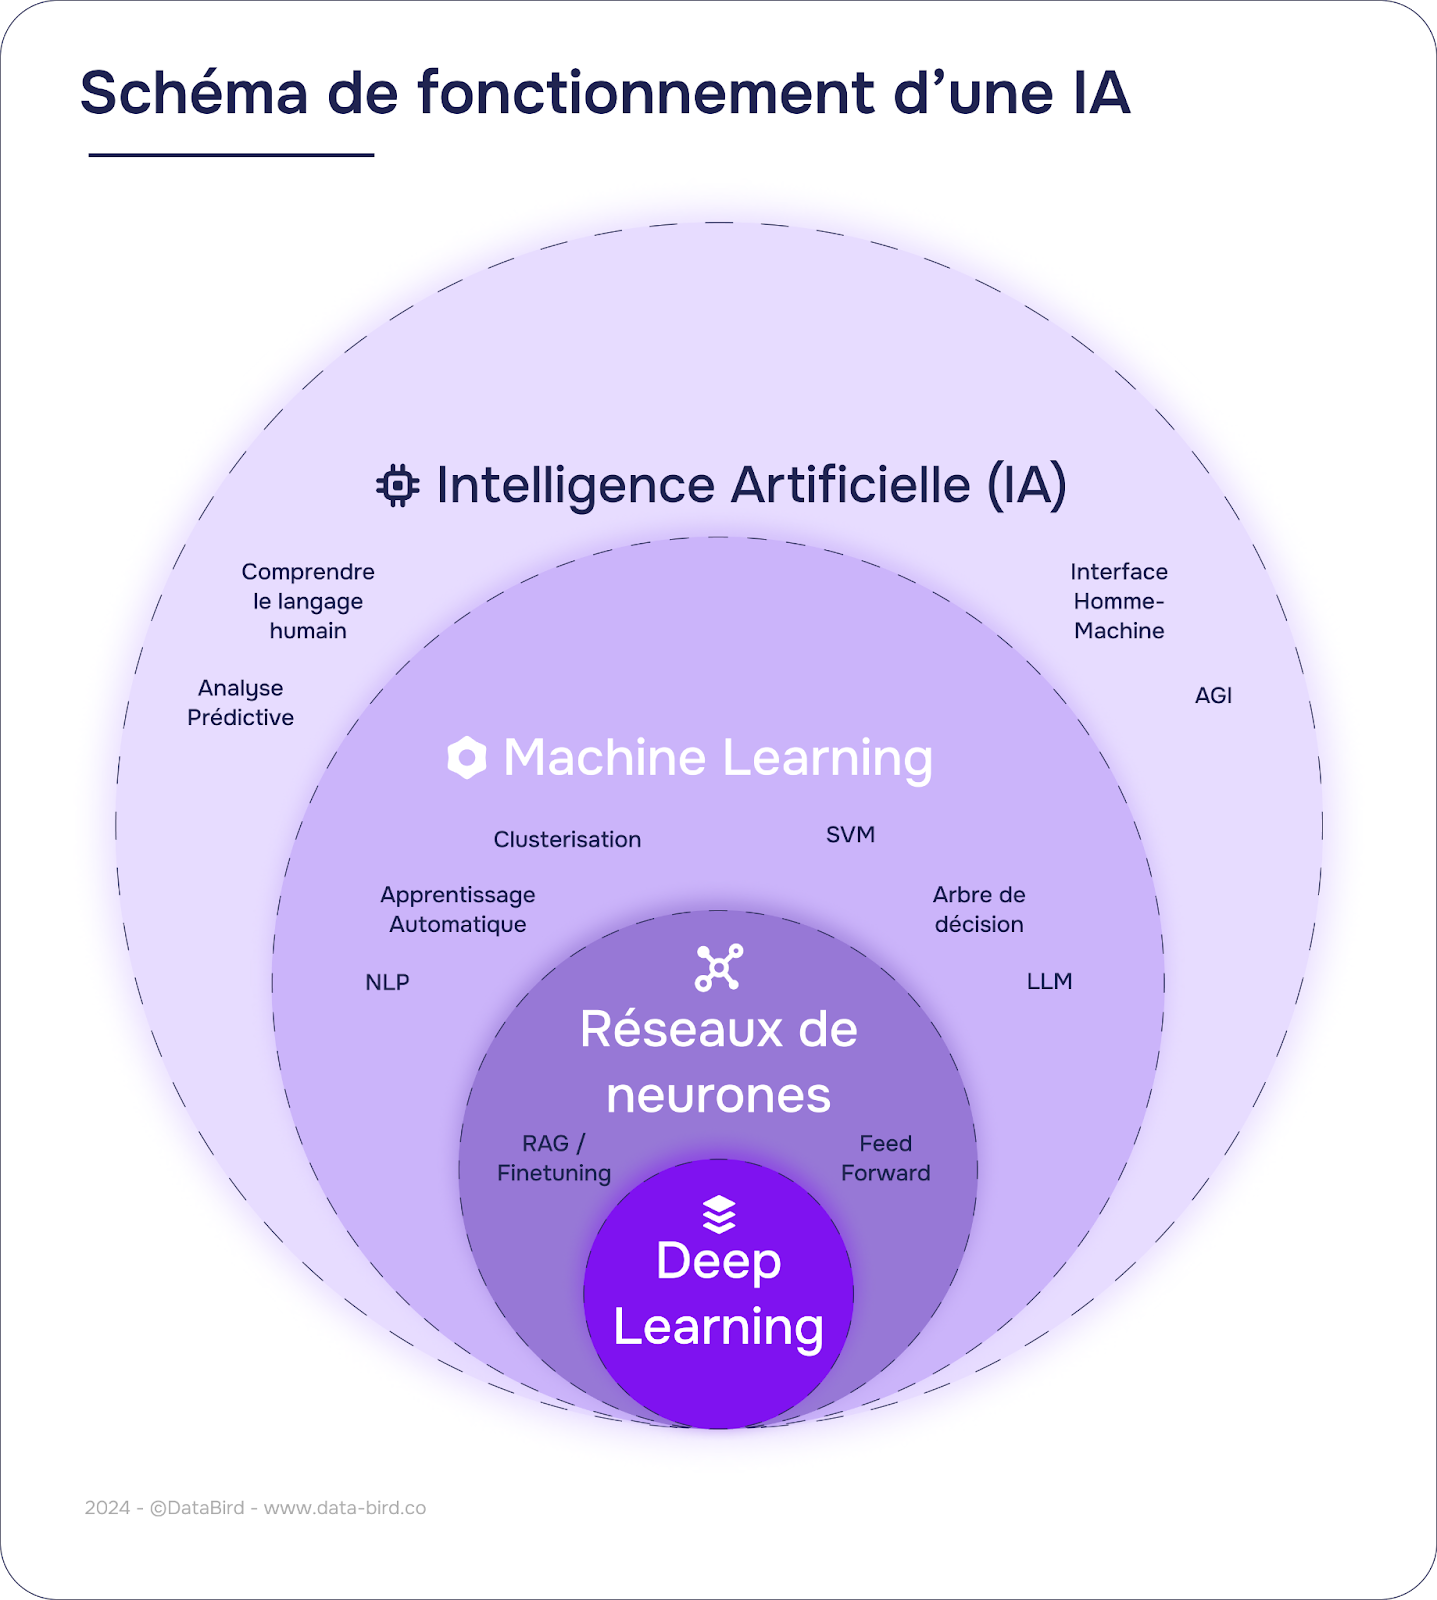
\includegraphics[width=0.7\textwidth]{images/2.1.1_2.png}
    \caption{Schéma d’intelligence artificielle}
    \label{fig:2.1.1_2}
\end{figure}

Je retiens que le fonctionnement de l’IA repose essentiellement sur trois piliers : les données, les modèles d’apprentissage et la capacité d’ajustement autonome. À partir de jeux de données volumineux et représentatifs, les systèmes d’IA construisent des modèles prédictifs ou classificatoires, souvent par le biais d’algorithmes d’apprentissage automatique, ou machine learning, qui leur permettent d’ajuster leurs paramètres internes en fonction des résultats obtenus. Ce processus, que je compare volontiers à une forme d’entraînement, consiste à minimiser les erreurs entre les prédictions du système et les résultats attendus, afin d’optimiser progressivement la performance. Les systèmes dits d’apprentissage profond, ou deep learning, franchissent une étape supplémentaire, en structurant les modèles sous forme de réseaux de neurones artificiels multicouches, capables d’extraire des représentations hiérarchiques et abstraites à partir des données brutes, comme l’expliquent clairement les auteurs du rapport de France Stratégie (2018)\footnote{France Stratégie 2018, Intelligence artificielle et travail : enjeux et perspectives. \cite{francestrategie}}.

Dans cette dynamique, je distingue plusieurs types d’intelligences artificielles, selon leur niveau de complexité et leur degré d’autonomie. Les IA dites faibles ou spécialisées sont conçues pour exécuter des tâches précises dans un domaine restreint, comme la reconnaissance vocale, la traduction automatique ou l’optimisation de calendriers. Elles n’ont pas de conscience ni de compréhension globale, mais elles peuvent surpasser les performances humaines dans certaines tâches bien définies. À l’opposé, les IA dites fortes, encore largement hypothétiques à ce jour, visent à reproduire l’ensemble des capacités cognitives humaines dans leur flexibilité, leur conscience d’elles-mêmes et leur capacité à apprendre de manière transversale. Cette distinction, que reprend l’équipe du CSE Québec (2020)\footnote{CSE Quebec 2020, L’intelligence artificielle en éducation \cite{hypotheses}}, me semble essentielle pour éviter toute confusion entre les applications concrètes actuelles et les projections spéculatives qui alimentent les discours médiatiques.

Enfin, je considère que l’intelligence artificielle n’est pas une entité autonome, mais une construction sociotechnique, inscrite dans des logiques de conception, de régulation et d’usage humain. Les systèmes intelligents n’apprennent pas seuls, mais à partir des données et des objectifs que je leur fournis. Leur efficacité, leur éthique et leur impact dépendent donc des choix que je fais en amont et de la vigilance que je maintiens dans leur déploiement. Cette vision, plus pragmatique que technocentrée, me permet d’aborder les enjeux liés à l’usage de l’IA dans le domaine de la mémorisation avec un regard équilibré, en tenant compte à la fois de ses promesses techniques et des conditions concrètes de son intégration dans les pratiques cognitives humaines.


%2.1.2
\subsection{IA faible vs IA forte}

Lorsque j’aborde les différentes formes que peut prendre l’intelligence artificielle, je suis amené à distinguer deux grandes catégories qui s’opposent tant par leur ambition que par leur degré de maturité technologique : d’un côté l’intelligence artificielle dite faible, qui désigne les systèmes spécialisés et opérationnels aujourd’hui, et de l’autre l’intelligence artificielle dite forte, qui relève encore du champ de la prospective et suscite autant d’espoir que de prudence.

\begin{figure}[h]
    \centering
    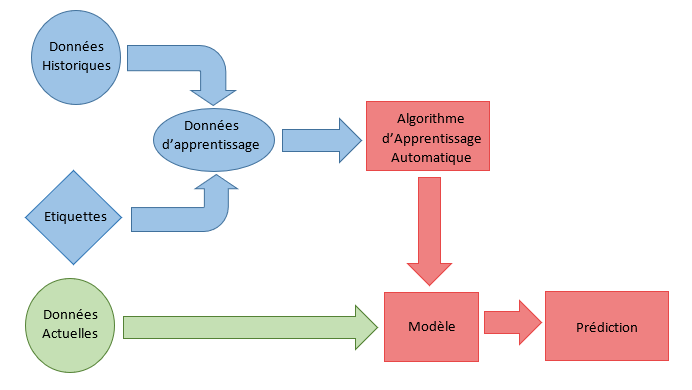
\includegraphics[width=0.7\textwidth]{images/2.1.1.png}
    \caption{Schéma des catégories d’intelligence artificielle}
    \label{fig:2.1.1}
\end{figure}

L’intelligence artificielle faible, parfois appelée IA étroite ou spécialisée, se caractérise par sa capacité à exécuter une tâche bien définie dans un domaine limité, sans aucune compréhension globale ni autonomie intellectuelle. Je constate que cette forme d’IA repose sur des algorithmes d’apprentissage automatique ou de traitement symbolique, qui exploitent des bases de données massives pour optimiser une fonction précise, comme reconnaître des visages, recommander des contenus, corriger un texte ou détecter des anomalies dans des données. Ces systèmes, bien qu’efficaces, ne sortent jamais du cadre pour lequel ils ont été conçus, et ils ne possèdent aucune intentionnalité propre. Ils apprennent par corrélation, mais ne construisent pas de représentations du monde comparables à celles que je peux élaborer en tant qu’être humain. Je les utilise quotidiennement dans des domaines aussi variés que la traduction, la navigation, l’analyse de texte ou la médecine prédictive, et je mesure à quel point leur efficacité repose sur une spécialisation extrême.

En revanche, l’intelligence artificielle forte, aussi appelée générale, désigne une hypothèse technologique selon laquelle un système artificiel pourrait non seulement accomplir une grande variété de tâches intellectuelles, mais aussi les transférer d’un domaine à un autre, avec une forme de compréhension et d’adaptation comparable à celle de l’intelligence humaine. Si cette forme d’IA venait à se concrétiser, elle pourrait théoriquement raisonner, apprendre de manière autonome, s’adapter à des situations inédites et même prendre conscience d’elle-même, ce qui soulèverait des enjeux éthiques, juridiques et sociaux majeurs. Pour l’heure, je constate que cette perspective reste largement spéculative, comme le souligne le rapport de la Commission de l’intelligence artificielle (2023)\footnote{Commission de l’intelligence artificielle. (2023). IA : notre ambition pour la France. Ministère de l’Économie et des Finances. \cite{iagouv}}, qui insiste sur le fait qu’aucun système actuel ne dispose de cette plasticité cognitive généralisée.

Je prends donc soin de ne pas confondre ces deux types d’intelligence artificielle, car cette confusion alimente des représentations biaisées et parfois anxiogènes du progrès technologique. L’IA faible est déjà présente dans mon quotidien et soulève des questions pratiques de régulation, de transparence et de responsabilité, tandis que l’IA forte, bien qu’elle nourrisse les imaginaires, demeure un horizon théorique qui me pousse à réfléchir aux limites que je souhaite poser à la délégation cognitive.

Cette distinction me paraît essentielle pour comprendre les usages potentiels de l’IA dans les domaines éducatifs et cognitifs, car seule une IA faible, encadrée, transparente et spécialisée peut aujourd’hui prétendre jouer un rôle utile dans l’assistance à la mémorisation, sans prétendre rivaliser avec mes facultés mentales dans leur ensemble.

%2.1.3
\subsection{Apprentissage automatique et réseaux de neurones}

Lorsque je cherche à comprendre comment les systèmes d’intelligence artificielle parviennent à résoudre des tâches complexes, comme la reconnaissance d’images, la traduction automatique ou encore la prédiction de comportements, je me tourne vers le principe fondamental de l’apprentissage automatique, aussi appelé machine learning, qui constitue aujourd’hui le socle de la grande majorité des applications d’IA.

\begin{figure}[h]
    \centering
    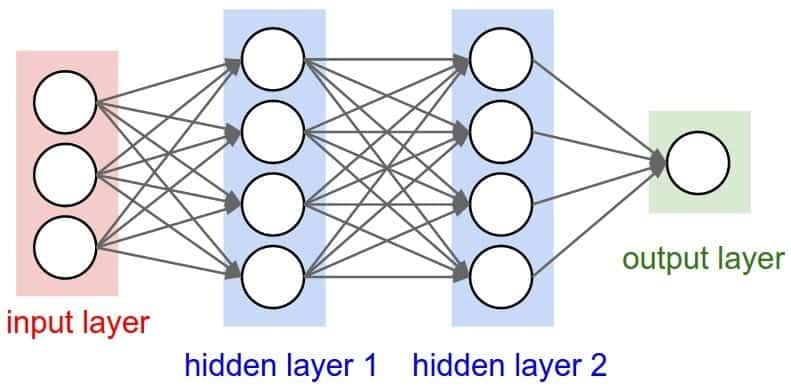
\includegraphics[width=0.7\textwidth]{images/2.1.3.png}
    \caption{Schéma d'un réseaux de neurones}
    \label{fig:2.1.3}
\end{figure}

L’apprentissage automatique repose sur l’idée qu’un système informatique peut améliorer ses performances à partir de données d’entraînement, sans avoir été explicitement programmé pour chaque cas de figure. En d’autres termes, ce système extrait des régularités, identifie des modèles et ajuste ses paramètres internes afin de minimiser l’écart entre ses prédictions et les résultats attendus. Je distingue plusieurs formes d’apprentissage, selon que les données soient annotées ou non. Lorsque les exemples incluent des réponses attendues, comme dans le cas d’images étiquetées « chat » ou « chien », il s’agit d’apprentissage supervisé ; en revanche, lorsque les données sont brutes et sans repères, je parle d’apprentissage non supervisé, où le système doit regrouper les éléments selon leurs similarités internes.

Je m’intéresse tout particulièrement à une forme d’apprentissage supervisé dite profonde, que l’on appelle apprentissage profond ou deep learning, qui repose sur des réseaux de neurones artificiels organisés en couches successives. Ces architectures s’inspirent du fonctionnement du cerveau humain dans leur logique de propagation d’un signal à travers des unités interconnectées. Chaque neurone artificiel effectue un calcul simple, mais l’agencement en couches permet au réseau de construire des représentations de plus en plus abstraites, depuis les traits élémentaires jusqu’aux concepts complexes. Ce fonctionnement, qui a été théorisé dès les années 1980 mais véritablement exploité à grande échelle à partir de la décennie 2010 grâce à l’augmentation de la puissance de calcul et des données disponibles, me permet aujourd’hui de bénéficier d’outils extrêmement performants dans des tâches cognitives automatisées.\footnote{Pensee Artificielle 2019, Comprendre LSTM et GRU : fonctionnement et schéma. \cite{penseeartificielle}}

Je note que ces réseaux de neurones profonds, bien qu’inspirés du cerveau humain, ne fonctionnent pas de manière biologique, mais mathématique. Ils apprennent par rétropropagation de l’erreur, c’est-à-dire en ajustant les poids des connexions entre les unités en fonction du résultat obtenu par rapport à la sortie attendue. Cette mécanique d’apprentissage par gradient descend, bien qu’efficace, n’implique aucune compréhension ni intentionnalité, ce qui m’oblige à rester vigilant face à l’illusion d’intelligence qui peut émerger lorsque les performances d’un système égalent ou surpassent celles d’un humain dans une tâche bien définie.\footnote{Octo. 2023. L'apprentissage profond : comprendre les réseaux de neurones \cite{octo}}

Comme l’explique clairement la CNIL dans son rapport sur l’IA et les données personnelles (2024)\footnote{CNIL 2024, Développement des systèmes d’IA : les recommandations de la CNIL pour respecter le RGPD. \cite{cnil}}, ces systèmes d’apprentissage automatique nécessitent de grandes quantités de données pour être entraînés, ce qui soulève des questions éthiques majeures quant à la confidentialité, à la traçabilité des informations utilisées et à la transparence des décisions algorithmiques. Je retiens donc que si les réseaux de neurones représentent un progrès remarquable en matière de traitement de l’information, leur utilisation dans des contextes cognitifs et éducatifs doit être encadrée, tant pour préserver les droits fondamentaux que pour éviter les biais systématiques que ces systèmes peuvent reproduire à grande échelle.

En comprenant le fonctionnement des réseaux de neurones et des algorithmes d’apprentissage, je me donne les moyens d’évaluer de manière critique les outils numériques qui en dérivent, et d’envisager leur intégration dans l’assistance à la mémorisation avec une conscience claire de leurs forces, de leurs limites et des responsabilités qu’ils impliquent.

%2.2
\section{Les assistants intelligents pour la mémoire}

%2.2.1
\subsection{Outils d’aide à la mémorisation basés sur l’IA}

Lorsque j’explore les applications concrètes de l’intelligence artificielle dans le domaine de la mémorisation, je découvre un ensemble d’outils numériques qui s’appuient sur des algorithmes d’apprentissage automatique pour adapter le contenu, le rythme et la forme des révisions à mes besoins cognitifs spécifiques. Ces dispositifs, qu’ils prennent la forme d’applications éducatives, de plateformes en ligne ou d’assistants personnalisés, utilisent des données issues de mon comportement d’apprentissage pour affiner en temps réel leur fonctionnement et améliorer ma rétention à long terme.

Parmi les solutions les plus emblématiques, je retiens les systèmes qui intègrent la répétition espacée algorithmique, comme Anki, SuperMemo ou encore les modules intelligents de Quizlet, qui analysent mes réussites, mes oublis et mes temps de réponse pour programmer mes révisions selon des intervalles optimaux. Ces outils, en appliquant de manière rigoureuse les principes issus des travaux d’Ebbinghaus sur la courbe de l’oubli, m’évitent de consacrer du temps à revoir des notions déjà bien consolidées, et concentrent au contraire mes efforts sur les connaissances fragiles ou récentes. Le CSE Québec (2020)\footnote{CSE Quebec 2020, L’intelligence artificielle en éducation \cite{hypotheses}} met en avant ce type d’approche comme l’une des formes les plus efficaces d’optimisation de l’apprentissage assisté par IA, notamment parce qu’elle permet de personnaliser l’expérience éducative à grande échelle.

Je remarque aussi que certains outils vont au-delà de la simple gestion du temps de révision, en intégrant des techniques de natural language processing, ou traitement automatique du langage, pour reformuler mes notes, générer des quiz personnalisés ou résumer automatiquement des contenus complexes. Ces fonctionnalités, que je retrouve dans des plateformes comme Notion AI, RemNote ou encore ChatGPT, contribuent à alléger ma charge cognitive en me proposant des formats synthétiques adaptés à mes préférences d’apprentissage. Grâce à l’analyse sémantique des documents que je fournis, ces systèmes parviennent à identifier les concepts centraux, les relations logiques entre les idées, et à me proposer des supports d’apprentissage structurés sans que j’aie à les construire moi-même.

Je m’intéresse également à l’émergence de tuteurs intelligents qui combinent des approches issues de la psychologie cognitive avec des algorithmes prédictifs pour me guider pas à pas dans l’acquisition d’une compétence ou la révision d’un programme. Ces systèmes, à l’image des assistants éducatifs développés dans les projets de recherche en EdTech, tentent de reproduire la dynamique d’un encadrement humain, en détectant les moments où je décroche, où je réussis trop facilement, ou encore où mes erreurs se répètent. Le rapport de la CNIL (2024)\footnote{CNIL 2024, Développement des systèmes d’IA : les recommandations de la CNIL pour respecter le RGPD. \cite{cnil}} attire toutefois mon attention sur le fait que ces technologies, pour fonctionner de manière pertinente, doivent accéder à des données personnelles parfois sensibles, comme mes rythmes d’étude, mes faiblesses conceptuelles ou mes niveaux de stress, ce qui pose des questions cruciales en matière de respect de la vie privée, de sécurité des données et de transparence des décisions algorithmiques.

Je retiens donc que les outils d’aide à la mémorisation fondés sur l’intelligence artificielle représentent une avancée significative en matière de personnalisation pédagogique, en me permettant d’adapter le contenu à mon rythme, de cibler mes lacunes et de renforcer ma motivation par une interaction dynamique. Toutefois, leur efficacité dépend largement de la qualité des données utilisées, de l’éthique de leur conception, et de ma propre capacité à les intégrer dans une démarche réflexive où la machine reste un soutien, et non un substitut, à mes efforts cognitifs.

%2.2.2
\subsection{Interfaces conversationnelles et assistants intelligents}

Lorsque j’interagis avec des outils numériques fondés sur le langage, je découvre que les interfaces conversationnelles, telles que les chatbots, les assistants vocaux ou les systèmes de type ChatGPT, transforment profondément ma manière d’accéder à l’information, d’organiser mes connaissances et de stimuler mes facultés de mémorisation. Ces dispositifs, reposant sur des modèles de traitement du langage naturel, sont capables de comprendre mes requêtes en langage courant, de me répondre de manière cohérente, et parfois même de générer des contenus personnalisés selon mes objectifs d’apprentissage ou les difficultés que je rencontre.

Je perçois que cette forme d’interaction, parce qu’elle se rapproche du dialogue humain, facilite l’engagement cognitif et émotionnel, deux leviers essentiels dans la mémorisation à long terme. Lorsque je pose une question à un assistant intelligent et que je reçois une réponse claire, structurée et immédiatement applicable, je mobilise mes capacités attentionnelles dans un cadre fluide, sans surcharge contextuelle, ce qui favorise l’encodage de l’information. Cette disponibilité permanente de l’outil, qui ne juge pas, ne fatigue pas, et s’adapte à mes horaires, me permet de m’exercer à tout moment, de reformuler mes incompréhensions, et de bénéficier d’un retour immédiat sur mes erreurs ou mes intuitions. C’est ce que met en avant Talan (2024), en soulignant que les interfaces conversationnelles représentent une nouvelle forme d’assistance cognitive, capable de réduire la charge mentale et de renforcer l’autonomie des apprenants.

Je remarque cependant que ces systèmes, bien qu’impressionnants dans leur fluidité linguistique, reposent sur des bases probabilistes et ne possèdent aucune compréhension véritable du sens ou de la logique sous-jacente à mes demandes. Leurs réponses sont le produit d’algorithmes statistiques qui calculent la suite de mots la plus probable en fonction des millions de textes sur lesquels ils ont été entraînés. Ce fonctionnement, comme l’explique la CNIL (2024), implique que les assistants conversationnels peuvent parfois fournir des informations inexactes, biaisées ou inappropriées, ce qui exige de ma part un esprit critique constant et une vérification systématique des contenus produits, surtout lorsqu’ils sont utilisés à des fins éducatives ou mémorielles.

Je dois aussi être conscient que ces systèmes conservent des traces de mes interactions, analysent mes préférences, et, dans certains cas, peuvent exploiter mes données pour améliorer leur performance globale ou pour orienter leurs suggestions futures. Cette dimension algorithmique, si elle est mal régulée, pourrait aboutir à une personnalisation excessive de mes usages, limitant l’ouverture de mon esprit à des informations nouvelles ou contradictoires. La CNIL alerte d’ailleurs sur ce risque de « bulle cognitive », où l’IA, en cherchant à me satisfaire, ne ferait que renforcer mes biais ou mes habitudes mentales, au détriment de la diversité intellectuelle.

Malgré ces précautions, je considère que les interfaces conversationnelles et les assistants intelligents représentent une avancée prometteuse dans l’accompagnement de la mémoire, en rendant l’apprentissage plus interactif, plus accessible et potentiellement plus motivant. Leur efficacité, toutefois, repose sur ma capacité à les intégrer dans un usage réfléchi, critique et encadré, où l’humain conserve la maîtrise de ses processus cognitifs, tout en tirant parti des facilités offertes par ces technologies dialogiques.

%2.2.3
\subsection{Réduction de la charge mentale}

Lorsque j’explore les innovations les plus récentes en matière de technologies éducatives, je constate que les dispositifs immersifs, comme la réalité virtuelle et la réalité augmentée, ainsi que les interfaces adaptatives, constituent des solutions prometteuses pour enrichir mes capacités de mémorisation en mobilisant simultanément mes sens, mes émotions et mon attention dans un environnement dynamique et engageant.

En expérimentant un environnement immersif, je me trouve plongé dans une simulation interactive où je peux manipuler des objets, interagir avec des éléments visuels et auditifs, et vivre des expériences proches du réel, sans les contraintes physiques ou les risques associés. Cette immersion sensorielle, en stimulant l’engagement émotionnel et corporel, renforce l’ancrage mnésique des contenus que je traite, car elle mobilise plusieurs modalités d’encodage de manière synchronisée. Le rapport de Startum (2023) met justement en lumière la capacité de la réalité virtuelle à activer des circuits cognitifs profonds, notamment dans l’apprentissage procédural ou contextuel, et à créer des souvenirs durables par la simulation d’expériences concrètes, que je n’aurais pas pu vivre dans un cadre classique.

Je remarque également que les interfaces adaptatives, en s’ajustant en temps réel à mon rythme, à mes erreurs, à mon niveau de fatigue ou de concentration, me proposent des parcours d’apprentissage sur mesure, qui évoluent en fonction de mes réponses et de mes interactions. Ces systèmes reposent sur des modèles prédictifs qui analysent mes performances pour ajuster la difficulté, le format ou la fréquence des exercices proposés. Ce type de personnalisation dynamique, qui repose sur l’intelligence artificielle, me permet d’éviter la frustration liée à une tâche trop complexe, tout en maintenant un niveau de stimulation suffisant pour renforcer ma motivation. Le Conseil supérieur de l’éducation du Québec (2020) souligne que ces interfaces adaptatives sont particulièrement efficaces pour soutenir les apprenants ayant des profils cognitifs atypiques, en leur offrant un environnement flexible, accessible et non stigmatisant.

Toutefois, je dois aussi m’interroger sur les conditions d’usage de ces technologies. Leur efficacité dépend non seulement de leur conception, mais aussi de l’accompagnement dont je bénéficie pour les utiliser. Sans un cadre pédagogique clair, ces outils risquent de me distraire plus qu’ils ne m’aident, ou de m’enfermer dans une logique de surstimulation qui entrave la consolidation de mes apprentissages. De plus, leur coût, leur accessibilité technique et leur compatibilité avec les infrastructures existantes constituent encore des freins à une généralisation équitable de leur usage. Le rapport Talan (2024) insiste d’ailleurs sur le risque de fracture numérique que ces technologies peuvent accentuer, en creusant l’écart entre les publics déjà familiarisés avec les outils numériques avancés et ceux qui en sont encore éloignés.

En définitive, je considère que les dispositifs immersifs et les interfaces adaptatives, s’ils sont bien intégrés dans un parcours d’apprentissage réfléchi, peuvent constituer de puissants leviers pour renforcer mes capacités de mémorisation, en transformant l’acte d’apprendre en une expérience multisensorielle, engageante et personnalisée. Néanmoins, leur usage ne peut se substituer à une réflexion pédagogique approfondie, ni à un accompagnement humain attentif, conditions essentielles pour que la technologie serve véritablement la cognition.

%2.3
\section{Les apports cognitifs de l’intelligence artificielle}

%2.3.1
\subsection{Accessibilité et inclusion cognitive grâce à l’IA}

Lorsque je réfléchis à la manière dont l’intelligence artificielle peut contribuer à rendre les environnements d’apprentissage plus inclusifs, je m’intéresse tout particulièrement à son potentiel en matière d’accessibilité cognitive, c’est-à-dire sa capacité à s’adapter aux besoins spécifiques des personnes présentant des troubles ou des limitations dans leurs fonctions mentales, qu’il s’agisse de difficultés d’attention, de mémoire, de compréhension ou de traitement de l’information.

J’observe que les systèmes d’IA, en raison de leur flexibilité algorithmique, peuvent analyser en temps réel mes comportements d’apprentissage, repérer mes zones de fragilité, et ajuster automatiquement la complexité, le rythme ou le format des contenus proposés, sans que j’aie à le signaler explicitement. Cette capacité d’adaptation silencieuse me permet de bénéficier d’un accompagnement personnalisé, non stigmatisant, qui respecte mon rythme cognitif sans exposer mes difficultés aux autres. Les travaux du CSE Québec (2020) soulignent à juste titre que cette forme d’intelligence adaptative constitue une avancée décisive pour les personnes présentant des troubles de l’apprentissage ou des handicaps cognitifs, en leur offrant un environnement ajusté à leurs compétences, et non l’inverse.

Je remarque également que l’IA peut faciliter l’accessibilité au savoir en diversifiant les formats d’entrée et de sortie des informations. Lorsque je peux écouter un texte au lieu de le lire, manipuler un concept à travers une simulation interactive ou transformer une consigne abstraite en image concrète, je multiplie les canaux d’accès à la compréhension, ce qui réduit les obstacles liés à la littératie, à la mémoire de travail ou à la représentation mentale. Ces modalités, accessibles grâce aux technologies de traitement du langage, de reconnaissance vocale ou de synthèse d’images, permettent à chacun de mobiliser ses points forts cognitifs au lieu de se heurter à ses limitations. Talan (2024) met ainsi en avant le rôle structurant de ces interfaces multisensorielles dans l’émancipation cognitive des publics éloignés des formats d’apprentissage standards.

Je dois toutefois rester vigilant sur deux plans. D’une part, l’efficacité de ces outils dépend fortement de la qualité des données qui les nourrissent. Si les bases d’entraînement ne prennent pas en compte la diversité cognitive, linguistique ou culturelle des apprenants, les systèmes risquent de reproduire des biais, d’exclure certains profils ou de proposer des aides inadaptées. D’autre part, je constate que l’accessibilité cognitive n’est pas uniquement une question de technologie, mais aussi de pédagogie, d’éthique et de politique publique. Rendre un dispositif techniquement accessible ne garantit pas son appropriation réelle par les personnes concernées, surtout si celles-ci manquent de ressources, de formation ou de confiance pour s’en emparer.

Ainsi, je considère que l’intelligence artificielle, loin de résoudre à elle seule les problèmes d’inclusion cognitive, constitue un levier puissant à condition d’être utilisée avec discernement, dans un cadre qui respecte les singularités cognitives, valorise l’autonomie des apprenants, et s’appuie sur une collaboration étroite entre concepteurs, professionnels de l’éducation, chercheurs et usagers.

%2.3.2
\subsection{Réduction de la charge mentale}

Lorsque j’évalue l’impact des technologies fondées sur l’intelligence artificielle dans le cadre de l’apprentissage et de la mémorisation, je reconnais que l’un des bénéfices les plus immédiats et les plus concrets réside dans leur capacité à réduire ma charge mentale, en m’aidant à mieux gérer les flux d’informations, à structurer mes tâches et à alléger les opérations cognitives redondantes ou dispersées.

La charge mentale, telle que définie par la théorie de la charge cognitive, désigne la quantité de ressources mentales que je dois mobiliser pour accomplir une tâche. Lorsque cette charge dépasse mes capacités de traitement, je perds en efficacité, en concentration et en mémorisation, car mon cerveau ne parvient plus à sélectionner, organiser et intégrer correctement les données. Ce phénomène, documenté dans les recherches reprises par l’Académie d’Aix-Marseille (2022), constitue l’un des principaux obstacles à l’apprentissage durable, surtout dans les environnements numériques saturés de stimuli visuels, auditifs et interactifs.

L’intelligence artificielle intervient à ce niveau en m’offrant des outils capables de filtrer l’information, de hiérarchiser les priorités et de proposer des supports d’aide qui réduisent la sollicitation inutile de ma mémoire de travail. Lorsque je reçois une explication simplifiée, un résumé contextuel ou une reformulation adaptée à mon niveau de compréhension, je libère de l’espace cognitif pour me concentrer sur l’essentiel, ce qui favorise l’encodage et la consolidation mnésique. Les interfaces conversationnelles, comme les assistants intelligents, participent également à cette décharge mentale en me guidant dans mes démarches, en anticipant mes besoins ou en automatisant des tâches répétitives, comme la création de rappels, la classification de documents ou la recherche ciblée d’informations.

Je remarque que cette réduction de la charge mentale ne se limite pas à l’allégement des contenus, mais concerne aussi la gestion de l’effort. Lorsque l’IA détecte que je commence à décrocher, que mes réponses se dégradent ou que mes temps de réaction s’allongent, elle peut ajuster le rythme, proposer une pause ou reformuler l’activité sous une autre forme, ce qui me permet de rester engagé sans m’épuiser. Le CSE Québec (2020) souligne cette capacité de régulation adaptative comme un atout essentiel dans les environnements d’apprentissage différenciés, où chaque apprenant présente une sensibilité particulière au stress, à la complexité ou à la surcharge cognitive.

Néanmoins, je dois rester conscient que cette aide, si elle est mal calibrée, peut produire un effet inverse en m’infantilisant ou en m’encourageant à déléguer excessivement mes efforts mentaux à la machine. Lorsque l’automatisation devient trop poussée, je risque de perdre l’habitude de structurer moi-même l’information, de planifier mes tâches ou de mobiliser activement mes stratégies mnésiques. C’est pourquoi je considère que la réduction de la charge mentale ne doit pas viser à éliminer l’effort cognitif, mais à en optimiser l’usage, en m’aidant à consacrer mes ressources aux activités réellement formatrices, tout en éliminant les distractions, les redondances et les surcharges inutiles.

Ainsi, j’en conclus que l’IA, lorsqu’elle est intégrée dans une logique d’accompagnement intelligent, peut agir comme un régulateur de ma charge mentale, me permettant de préserver mon attention, de renforcer ma mémorisation et de progresser avec plus de fluidité dans mes apprentissages, à condition de rester acteur de ce processus et non simple utilisateur passif de ses résultats.

%2.3.3
\subsection{Personnalisation et motivation}

Lorsque je m’interroge sur les raisons qui me poussent à m’investir durablement dans un apprentissage, je reconnais que la motivation, qu’elle soit intrinsèque ou extrinsèque, joue un rôle central dans ma capacité à retenir, à comprendre et à transférer des connaissances. Je remarque que l’intelligence artificielle, en adaptant dynamiquement les contenus et les modalités d’apprentissage à mes besoins, à mes préférences et à mes rythmes, peut renforcer cette motivation en créant un environnement perçu comme plus engageant, plus accessible et plus valorisant.

Grâce aux systèmes adaptatifs intégrés dans de nombreuses applications d’apprentissage, je bénéficie d’une personnalisation de plus en plus fine, qui prend en compte non seulement mon niveau de compétence initial, mais aussi ma progression, mes erreurs récurrentes, mes domaines de prédilection et mes stratégies préférées. Cette personnalisation ne se limite pas à une simple adaptation de la difficulté, mais touche aussi la forme des supports, le type d’activités proposées et la fréquence des interactions. En me sentant compris et accompagné dans ma singularité cognitive, je développe un sentiment de compétence et d’auto-efficacité, deux facteurs essentiels pour nourrir une motivation durable. Le CSE Québec (2020) souligne à cet égard que l’IA permet une pédagogie différenciée à grande échelle, capable de répondre à des profils très variés, y compris ceux que les dispositifs classiques peinent à intégrer.

Je note aussi que la personnalisation par l’IA contribue à rendre les apprentissages plus concrets et plus significatifs, en m’aidant à faire des liens entre mes intérêts personnels, mes objectifs de formation et les savoirs à acquérir. Lorsque je peux explorer un sujet à travers des exemples qui résonnent avec mes expériences, ou quand un système intelligent me propose un défi à la mesure de mes capacités, je me sens davantage impliqué dans l’activité, ce qui augmente ma concentration et mon engagement émotionnel. Cette implication active, en retour, favorise l’encodage profond et la consolidation mnésique, comme le montrent les principes de la psychologie cognitive appliqués à l’apprentissage.

Cependant, je reste lucide face aux limites d’une personnalisation fondée uniquement sur des données comportementales. Si l’algorithme ne prend en compte que mes performances passées pour me recommander du contenu, il risque de me cantonner à des zones de confort, en négligeant les moments où je pourrais avoir besoin d’être confronté à des situations nouvelles, inconfortables ou déstabilisantes pour apprendre véritablement. Talan (2024) met en garde contre cet effet de boucle algorithmique, où la personnalisation excessive finit par appauvrir la diversité des apprentissages et réduire ma capacité à m’adapter à des environnements imprévus.

En définitive, je considère que la personnalisation permise par l’intelligence artificielle, si elle est bien conçue, me permet d’apprendre à mon rythme, selon mes modalités préférées, tout en renforçant ma motivation et ma persévérance. Mais pour que cette personnalisation soit réellement bénéfique, elle doit rester ouverte, évolutive, et s’accompagner d’un cadre réflexif qui me permette de garder la maîtrise de mes apprentissages, sans me reposer uniquement sur des recommandations automatisées.

%3
\chapter{Développement d’un système intelligent d’aide à la mémorisation}

%3.1
\section{Choix technologiques et fondements algorithmiques}

%3.1.1
\subsection{Traitement automatique du langage naturel (NLP) et enjeux cognitifs}

Lorsque je cherche à concevoir un système intelligent capable d’assister efficacement l’utilisateur dans ses efforts de mémorisation, je me rends rapidement compte que la compréhension, l’analyse et la transformation du langage naturel constituent une étape centrale du processus. En effet, si je souhaite que l’intelligence artificielle identifie les points clés d’un texte, reformule des notions complexes, ou génère des questions pour aider à la rétention, elle doit être en mesure de traiter le langage humain sous toutes ses dimensions : syntaxiques, sémantiques, contextuelles et pragmatiques.

Le traitement automatique du langage naturel, que je désigne par le sigle NLP (Natural Language Processing), regroupe un ensemble de techniques algorithmiques visant à permettre à une machine de manipuler et de produire du texte de manière intelligible. Ces techniques incluent notamment l’analyse morphologique, la reconnaissance d’entités nommées, la vectorisation sémantique ou encore la génération de texte. À travers le NLP, je peux transformer un document brut en une séquence d’unités exploitables par un modèle d’apprentissage automatique, tout en conservant la richesse et la structure du langage naturel.

Je m’appuie dans cette perspective sur des outils de prétraitement tels que la tokenisation, qui consiste à segmenter le texte en unités lexicales pertinentes, le lemmatisation, qui réduit chaque mot à sa forme canonique, et la vectorisation, qui convertit les mots en vecteurs numériques capables de représenter leurs relations sémantiques dans un espace multidimensionnel. Parmi les méthodes de vectorisation, je retiens l’usage de word embeddings comme Word2Vec ou GloVe, qui permettent de capturer les similarités de sens entre mots, et les techniques plus récentes comme BERT, qui tiennent compte du contexte bidirectionnel d’un mot dans une phrase, renforçant ainsi la précision des représentations sémantiques.

En intégrant ces outils dans la conception de mon système, je vise à ce que l’intelligence artificielle puisse extraire automatiquement les concepts clés d’un texte, les relier à des notions préexistantes dans la mémoire de l’utilisateur, et proposer des reformulations, des résumés ou des exercices adaptés pour consolider ces connaissances. Le NLP devient ainsi un pont entre l’univers symbolique du langage humain et le traitement numérique par l’IA, un vecteur essentiel pour que le système d’aide à la mémorisation soit réellement pertinent, réactif et personnalisé.

Je considère que ce recours au traitement du langage naturel ne se limite pas à une fonctionnalité technique, mais constitue un prolongement des processus cognitifs humains. En donnant à la machine la capacité de traiter le langage comme je le fais intuitivement, je renforce non seulement son efficacité technique, mais aussi sa capacité à interagir de manière naturelle et pédagogique avec l’utilisateur.

%3.1.2
\subsection{Justification du choix des réseaux LSTM et GRU}

Lorsque je cherche à concevoir un système intelligent capable de modéliser des séquences de texte à des fins de mémorisation, je me rends vite compte que l’un des défis majeurs réside dans la capacité du modèle à prendre en compte la temporalité, la dépendance entre les éléments d’une séquence, et la récurrence des informations. Un simple réseau de neurones artificiels traditionnel, bien qu’efficace pour les tâches de classification statique, ne suffit pas à capter la dynamique du langage naturel, où chaque mot dépend du contexte dans lequel il est inséré, parfois plusieurs phrases auparavant. C’est pourquoi je choisis de me tourner vers les réseaux neuronaux récurrents, ou RNN, qui sont conçus pour traiter les données séquentielles en conservant une mémoire des états précédents.

Cependant, les RNN classiques présentent des limitations structurelles importantes, notamment lorsqu’il s’agit de traiter des séquences longues. En pratique, je constate que ces modèles souffrent de ce que l’on appelle le problème du gradient qui disparaît ou explose, rendant l’apprentissage instable ou inefficace lorsque les dépendances temporelles dépassent quelques unités. Pour remédier à cette difficulté, je choisis d’utiliser des architectures de réseaux récurrents améliorées, en particulier les réseaux LSTM (Long Short-Term Memory) et GRU (Gated Recurrent Unit), qui ont été spécifiquement conçus pour maintenir l’information sur de longues séquences et mieux réguler le flux d’apprentissage.

Les réseaux LSTM, introduits par Hochreiter et Schmidhuber en 1997, s’appuient sur une structure interne plus complexe que celle des RNN standards. Je note qu’ils intègrent des portes de contrôle (input, forget, output) qui permettent de décider, à chaque étape temporelle, quelles informations doivent être mémorisées, oubliées ou transmises à l’état suivant. Cette architecture me permet de modéliser avec précision des séquences linguistiques, en conservant les éléments significatifs du passé tout en actualisant les états internes au fil de la lecture du texte. Ce fonctionnement me semble particulièrement pertinent pour des tâches liées à la mémorisation, comme la reformulation de contenu, le suivi des rappels ou la détection des concepts clés.

Les réseaux GRU, quant à eux, constituent une variante plus récente et plus légère des LSTM, proposée par Cho et al. en 2014. En simplifiant l’architecture interne par la fusion de certaines portes, ils offrent une efficacité computationnelle supérieure, ce qui les rend attractifs dans un contexte de prototypage rapide ou d’intégration dans des applications à ressources limitées. Bien que légèrement moins performants sur certaines tâches complexes, ils conservent une capacité d’apprentissage séquentiel robuste, tout en réduisant le temps d’entraînement.

Mon choix de travailler avec ces deux architectures repose donc sur un compromis entre fidélité temporelle, stabilité de l’apprentissage et efficacité opérationnelle. En expérimentant ces modèles sur des jeux de données textuels liés à la mémorisation (par exemple des séries de questions-réponses, des résumés de textes ou des mots-clés extraits), je peux analyser leur aptitude à prédire les contenus oubliés, à générer des rappels intelligents ou à proposer des contenus reformulés selon l’historique de l’utilisateur.

Je considère ainsi que l’intégration de réseaux LSTM ou GRU constitue une base solide pour construire un système de mémorisation intelligent, car ces architectures permettent à la machine de « se souvenir » de l’information utile tout en filtrant ce qui peut être négligé, à l’image du fonctionnement adaptatif de la mémoire humaine.

%3.2
\section{Méthodologie de conception du système}

%3.2.1
\subsection{Préparation des données et stratégie d’entraînement du modèle}

Avant de pouvoir entraîner un modèle de réseau LSTM ou GRU dans le but de concevoir un système intelligent d’aide à la mémorisation, je dois porter une attention rigoureuse à la préparation des données textuelles qui vont nourrir ce modèle. En effet, la qualité et la structuration des données d’entrée constituent la fondation sur laquelle repose l’apprentissage, car un algorithme, aussi performant soit-il, ne pourra produire des résultats pertinents que s’il est exposé à des séquences cohérentes, représentatives et nettoyées.

Je commence par sélectionner un corpus textuel adapté à la tâche visée, c’est-à-dire un ensemble de contenus dans lequel les mécanismes de mémorisation peuvent s’appliquer de manière concrète. Ce corpus peut inclure des extraits pédagogiques, des définitions, des résumés de chapitres, des flashcards ou encore des dialogues de questions-réponses. Je veille à ce que les textes couvrent différents niveaux de difficulté, divers styles rédactionnels et une variété suffisante de sujets, afin de permettre au modèle d’apprendre à généraliser les stratégies d’encodage et de rappel dans différents contextes d’apprentissage.

Une fois le corpus constitué, je procède à une phase de prétraitement indispensable pour rendre les données exploitables par le réseau neuronal. Cette étape inclut la normalisation des caractères (suppression des accents, conversion en minuscules), la suppression des ponctuations inutiles, la tokenisation en unités lexicales (mots ou sous-mots), et éventuellement la lemmatisation ou la racinisation pour réduire les variations morphologiques. J’applique ensuite une technique de vectorisation, telle que l’encodage one-hot ou l’utilisation d’un embedding pré-entraîné comme GloVe ou Word2Vec, qui me permet de représenter chaque mot sous forme d’un vecteur dense, porteur d’une information sémantique contextuelle.

Pour entraîner le modèle, je transforme ces données vectorisées en séquences temporelles glissantes, où chaque entrée contient une phrase tronquée et l’objectif du réseau est de prédire le mot ou l’expression suivante. Cette tâche, connue sous le nom de langage conditionnel, constitue un fondement du fonctionnement des LSTM et GRU. Je veille à définir une taille de séquence cohérente, ni trop courte pour ne pas perdre le contexte, ni trop longue pour ne pas diluer la pertinence du signal. J’intègre également un mécanisme de masquage afin de gérer les longueurs variables dans les batchs d’entraînement.

En parallèle, je définis une stratégie d’entraînement adaptée à la complexité du modèle et à la nature des données. Je sélectionne une fonction de coût pertinente (généralement l’entropie croisée pour la classification de mots), un optimiseur efficace comme Adam, et un taux d’apprentissage progressif pour éviter les phénomènes de surapprentissage ou de stagnation. J’introduis un système de validation croisée et d’arrêt anticipé basé sur la perte de validation pour m’assurer que le modèle apprend de manière stable sans se suradapter aux données d’entraînement.

L’ensemble de cette méthodologie me permet de mettre en place un pipeline reproductible et robuste, où les données sont préparées, enrichies et utilisées pour entraîner un modèle qui sera ensuite évalué sur sa capacité à simuler, anticiper ou compléter des processus cognitifs de mémorisation. En procédant de manière rigoureuse à cette phase initiale, je pose les bases d’un système dont l’intelligence réside moins dans la complexité algorithmique que dans la qualité et la cohérence du traitement du langage sur lequel il s’appuie.

%3.2.2
\subsection{Simulation de rappels intelligents et prédiction des oublis}

Une fois le modèle entraîné à reconnaître et à traiter des séquences textuelles, je m’oriente vers l’intégration d’une fonctionnalité essentielle pour mon projet : la simulation de rappels intelligents, qui consiste à générer automatiquement des suggestions de révision ciblées, adaptées au niveau de consolidation mnésique de l’utilisateur. Cette fonctionnalité repose sur la capacité du système à identifier les zones de fragilité cognitive, à estimer la probabilité d’oubli, et à proposer des rappels au moment optimal pour renforcer la mémorisation sans générer de surcharge.

Pour construire ce mécanisme, je m’inspire des principes de la répétition espacée, théorisés initialement par Ebbinghaus et largement repris dans les algorithmes modernes tels que ceux de SuperMemo. Le modèle que je développe intègre une composante temporelle qui permet de suivre l’historique des interactions d’un utilisateur avec un contenu donné : à chaque fois qu’un concept est étudié, rappelé ou oublié, une mise à jour de sa “trace mnésique” est effectuée. Je combine ces données temporelles avec les sorties du réseau LSTM ou GRU pour calculer une fonction de score qui reflète le degré de maîtrise estimé de chaque information.

Ce score, que je modélise comme une probabilité d’oubli, me permet d’ordonner les contenus selon leur priorité de révision. Lorsque cette probabilité dépasse un certain seuil, le système déclenche un rappel intelligent, sous forme de question, de reformulation, ou de carte de mémorisation, en s’appuyant sur les capacités génératives du modèle pour varier les formulations et contextualiser l’exercice. Cette variation est essentielle pour éviter l’effet de reconnaissance mécanique et stimuler une récupération active, facteur clé du renforcement mnésique.

Je veille également à ce que le système tienne compte non seulement de la fréquence des révisions, mais aussi de leur espacement dans le temps, de la difficulté du contenu et du niveau de confiance exprimé par l’utilisateur s’il interagit avec une interface autoévaluative. En analysant ces variables conjointement, le modèle devient capable non seulement de réagir à l’oubli, mais aussi de le prédire, en estimant à quel moment une notion risque d’être oubliée, selon la dynamique propre à chaque utilisateur.

Je m’appuie pour cela sur des architectures hybrides, qui combinent la mémoire interne des LSTM ou GRU avec des unités de suivi temporel externe, telles que des vecteurs horodatés ou des embeddings temporels. Ces éléments permettent d’intégrer dans le calcul du modèle non seulement le contenu sémantique, mais aussi les régularités temporelles propres au comportement d’étude de l’utilisateur.

En intégrant ce mécanisme prédictif dans mon système, je transforme le réseau neuronal en un assistant proactif, qui n’attend pas que l’oubli soit manifeste pour intervenir, mais qui anticipe les défaillances de la mémoire en les modélisant comme des événements probabilistes. Ce type de fonctionnement me semble particulièrement pertinent dans les environnements éducatifs ou thérapeutiques, où la régularité et la pertinence des rappels peuvent faire la différence entre un apprentissage superficiel et une acquisition durable des connaissances.

Ainsi, en simulant intelligemment les rappels et en anticipant les oublis, je permets à mon système d’agir comme un facilitateur mnésique personnalisé, qui s’adapte en temps réel aux besoins cognitifs de l’utilisateur, tout en respectant ses rythmes, ses préférences et son historique d’apprentissage.

%3.2.3
\subsection{Interface d’usage et scénario utilisateur}

Pour que le système intelligent que je conçois ne reste pas à l’état de démonstration algorithmique mais devienne un véritable outil d’aide à la mémorisation accessible et pertinent, je dois penser une interface d’usage qui facilite son intégration dans le quotidien de l’utilisateur. Cette interface constitue la jonction entre la complexité du traitement algorithmique sous-jacent et la simplicité attendue dans l’expérience utilisateur. Elle doit permettre d’interagir intuitivement avec le système, de suivre ses recommandations, d’exprimer ses besoins, et d’obtenir un retour compréhensible sur les progrès accomplis.

Dans le cadre de cette conception, je privilégie une interface web ou mobile épurée, centrée sur l’essentiel, où l’utilisateur est accueilli par un tableau de bord synthétique lui indiquant les contenus à réviser, les notions récemment consolidées, les rappels à venir, et un indicateur visuel de sa progression mnésique. Chaque contenu proposé s’accompagne d’un rappel interactif sous forme de question, d’exercice ou de carte mémoire, généré dynamiquement par le modèle à partir du corpus initial, en tenant compte des reformulations nécessaires pour éviter la redondance mécanique.

Je choisis également d’intégrer une fonction de dialogue assisté, où l’utilisateur peut interroger le système en langage naturel, demander des explications, reformuler un contenu qu’il ne comprend pas, ou encore solliciter une version simplifiée. Cette fonctionnalité repose sur les capacités de NLP intégrées en amont, et permet de personnaliser les interactions de manière fluide et non rigide, ce qui contribue à renforcer l’engagement dans l’apprentissage.

Du point de vue du scénario utilisateur, je conçois un cycle d’interaction quotidien où l’utilisateur consulte sa liste de rappels, répond à des sollicitations générées par le système, et bénéficie d’une évaluation progressive de ses réponses. En cas d’échec répété ou d’incertitude exprimée, le modèle réajuste la fréquence de révision de cette notion et reformule l’information pour en faciliter la compréhension. Au contraire, en cas de réussite stable sur un contenu donné, le système espace les rappels et passe à des concepts connexes, favorisant l’élargissement du champ de mémorisation.

Je veille à ce que l’interface permette également à l’utilisateur de consulter son historique d’apprentissage, sous la forme de graphiques ou de tableaux interactifs, lui montrant non seulement ce qu’il sait, mais aussi ce qu’il a oublié ou renforcé. Cette visualisation de la mémoire, bien qu’artificielle, renforce la métacognition, en rendant visibles les processus internes de l’apprentissage, et en encourageant l’auto-régulation.

Enfin, je m’assure que l’interface respecte les critères d’accessibilité universelle, afin que le système puisse être utilisé par des publics variés, y compris ceux présentant des troubles cognitifs ou des limitations sensorielles. Cela inclut des options de synthèse vocale, de taille de police ajustable, de contraste élevé, et une navigation simplifiée. Je fais également en sorte que les données personnelles, les performances et les préférences de l’utilisateur soient protégées selon les principes du RGPD, en intégrant des systèmes d’anonymisation et de contrôle de la confidentialité.

Ainsi, en concevant une interface orientée vers l’expérience cognitive de l’utilisateur et un scénario d’usage rythmé mais adaptable, je m’efforce de faire de ce modèle un véritable assistant intelligent de mémorisation, non seulement performant sur le plan technique, mais aussi intégré à une logique pédagogique respectueuse, évolutive et centrée sur l’humain.

%3.3
\section{Entraînement du modèle et évaluation des performances}

%3.3.1
\subsection{Critères d’évaluation du modèle}

Lorsque je cherche à évaluer l’efficacité du système d’assistance à la mémorisation que j’ai conçu, je ne peux me contenter d’une simple vérification de son bon fonctionnement technique. Je dois mettre en place une série de critères d’évaluation qui me permettent de mesurer, de manière objective et reproductible, la pertinence, la précision et l’utilité cognitive réelle du modèle développé. Ces critères ne se limitent pas à des métriques informatiques classiques, mais doivent être pensés en lien avec la finalité pédagogique du projet : favoriser la rétention d’information, adapter les rappels aux besoins, et alléger la charge mentale de l’utilisateur.

Le premier critère que je considère est celui de la précision des prédictions, notamment dans le cadre de la génération de rappels. Il s’agit ici d’évaluer si le système est capable de proposer, à partir d’un historique d’interactions, les contenus les plus pertinents à rappeler, au moment le plus opportun. Pour cela, je mesure la précision au top-k, qui m’indique la proportion de fois où le contenu effectivement oublié ou mal consolidé par l’utilisateur figure parmi les k suggestions prioritaires du modèle. Cette métrique me permet d’estimer à quel point le système cible correctement les failles mnésiques.

Le second critère repose sur la capacité d’adaptation du modèle, c’est-à-dire sa faculté à personnaliser les séquences d’apprentissage en fonction du profil cognitif et comportemental de l’utilisateur. Je mesure cette adaptabilité par la comparaison de performances entre utilisateurs ayant des rythmes, des niveaux ou des préférences différents, en analysant si le système maintient un taux de rappel élevé tout en modulant ses propositions. Une bonne adaptabilité se traduit par une amélioration du score mnésique, calculé à partir de la rétention moyenne des contenus sur plusieurs sessions, quel que soit le type d’utilisateur.

Un troisième critère essentiel est celui du temps de réponse du système, qui ne doit pas entraver l’expérience utilisateur. J’évalue ici la latence moyenne entre une requête utilisateur (comme une demande de rappel ou de reformulation) et la réponse générée par le modèle. En utilisant des architectures LSTM ou GRU optimisées, je vise un temps de traitement inférieur à une seconde dans un contexte applicatif en ligne. Ce critère me semble fondamental car un délai trop important peut briser la dynamique cognitive de l’utilisateur et nuire à l’efficacité de l’apprentissage.

Enfin, j’introduis un indicateur composite de satisfaction utilisateur simulée, qui combine les taux de réponse correcte, le niveau d’engagement (nombre d’interactions volontaires) et les signaux comportementaux comme le taux d’abandon ou le retour vers un contenu antérieur. Ces éléments, bien qu’indirects, me permettent d’évaluer si le système remplit bien son rôle d’assistant cognitif, non seulement sur le plan algorithmique, mais aussi en termes d’expérience vécue.

En articulant ces critères, je peux affiner les performances du système au-delà de la simple exactitude, en les confrontant aux exigences d’un outil éducatif destiné à accompagner la mémoire humaine. Cette évaluation me permet aussi d’identifier les points faibles du modèle, et d’ajuster les paramètres ou les mécanismes internes pour renforcer son efficacité dans un usage réel.

%3.3.2
\subsection{Limites rencontrées et ajustements du modèle}

Au cours du développement et de l’entraînement du système d’aide à la mémorisation, je me suis confronté à plusieurs limites techniques, structurelles et méthodologiques, qui m’ont conduit à ajuster certains paramètres et à repenser ponctuellement des choix initiaux. Ces limites, loin de remettre en cause la pertinence du projet, m’ont permis d’affiner mon approche, de mieux comprendre les contraintes réelles d’un modèle séquentiel de type LSTM ou GRU, et d’améliorer l’adéquation entre la logique algorithmique et les objectifs cognitifs poursuivis.

L’une des premières difficultés majeures que j’ai rencontrées concerne le surapprentissage, phénomène bien connu dans l’entraînement de réseaux neuronaux, qui se manifeste lorsque le modèle mémorise les données d’entraînement de manière trop précise, au détriment de sa capacité à généraliser. Ce problème s’est posé particulièrement dans les premières itérations, lorsque le corpus textuel utilisé était trop homogène ou trop limité en termes de diversité lexicale et syntaxique. Pour y remédier, j’ai intégré plusieurs techniques de régularisation, notamment le dropout, qui désactive aléatoirement certaines unités neuronales pendant l’apprentissage, et j’ai élargi le corpus avec des sources variées afin de renforcer la robustesse des représentations apprises.

Une autre limite, plus subtile, réside dans la gestion des séquences longues, que les architectures LSTM et GRU, bien qu’optimisées, peinent encore à traiter au-delà d’un certain seuil. Lorsque la dépendance contextuelle dépasse vingt ou trente unités lexicales, je constate une perte de cohérence dans les prédictions du modèle, liée à l’affaiblissement du signal de mémoire interne. Pour atténuer ce phénomène, j’ai réduit la taille des séquences d’entrée tout en conservant un découpage logique (phrases complètes ou segments sémantiques), et j’ai envisagé l’usage de mécanismes d’attention pour mieux pondérer l’importance relative des éléments de la séquence, bien que cela sorte du périmètre initial du projet.

J’ai également dû ajuster plusieurs hyperparamètres fondamentaux tels que le taux d’apprentissage, la taille des batchs, le nombre d’unités cachées ou le nombre d’époques d’entraînement. Ces ajustements, que j’ai réalisés de manière itérative à l’aide de techniques de recherche manuelle et semi-automatisée, ont eu un impact direct sur la stabilité du modèle et la convergence de la fonction de perte. Un taux d’apprentissage trop élevé entraînait des oscillations autour du minimum global, tandis qu’un taux trop faible ralentissait inutilement la progression. Le bon compromis s’est situé, dans mon cas, autour de 0.001 avec l’optimiseur Adam.

Enfin, j’ai observé certaines limites dans l’interprétabilité du modèle. Bien que les LSTM et GRU soient plus transparents que d’autres architectures plus complexes, ils restent fondamentalement des “boîtes noires” dans leur fonctionnement interne. Cette opacité rend difficile l’explication des décisions prises par le système, par exemple lorsqu’un rappel est généré de manière inattendue. Pour pallier ce manque de transparence, j’ai mis en place des visualisations des activations internes et j’ai documenté chaque étape du traitement pour permettre une relecture pédagogique du fonctionnement.

Ainsi, en identifiant ces contraintes et en y répondant par des ajustements ciblés, j’ai progressivement stabilisé un modèle fonctionnel, capable d’accompagner l’utilisateur dans ses processus de mémorisation avec une relative efficacité. Ces limites, loin de disqualifier l’approche, me rappellent que le développement d’un système intelligent ne repose pas uniquement sur la puissance algorithmique, mais aussi sur une compréhension fine des contextes d’usage, des comportements cognitifs, et des marges de tolérance des utilisateurs réels.

%3.4
\section{Scénarios d’utilisation et perspectives d’amélioration}

%3.4.1
\subsection{Cas d’usage avancé}

Pour illustrer la pertinence et la faisabilité de mon système intelligent d’assistance à la mémorisation, je propose un cas d’usage avancé qui simule l’intégration de ce dispositif dans le cadre d’une plateforme d’apprentissage destinée à des étudiants préparant des examens à forte charge théorique, comme ceux des disciplines médicales, juridiques ou scientifiques. Dans ce contexte, les apprenants doivent assimiler une grande quantité d’informations structurées, les réviser régulièrement, et être capables de les mobiliser en situation d’évaluation, ce qui constitue un terrain d’application idéal pour le modèle que j’ai conçu.

Je me place dans le scénario suivant : un étudiant en première année de médecine utilise quotidiennement une application de révision personnalisée, intégrant mon système basé sur des réseaux LSTM pour la prédiction des oublis, et un moteur de génération NLP pour la création de rappels intelligents. Lorsqu’il se connecte, l’application lui présente une interface adaptée à son rythme, où sont affichées les notions à revoir en priorité, accompagnées de questions générées automatiquement à partir des textes de cours importés précédemment.

À chaque interaction, le système enregistre la réponse de l’utilisateur, le temps de réponse, le niveau de confiance autoévalué, et l’historique des réussites ou échecs. Ces données alimentent un module interne qui ajuste dynamiquement le score de mémorisation associé à chaque notion, et détermine la fréquence de rappel idéale pour maintenir une consolidation optimale. Par exemple, si l’étudiant échoue à rappeler une définition vue la veille, le système réintègre cette notion dans le cycle de révision du jour suivant, en modifiant sa formulation ou en l’insérant dans un contexte clinique nouveau, afin de favoriser un encodage plus profond.

Ce cas d’usage montre que le modèle ne se contente pas de mesurer des performances passives, mais s’engage activement dans la progression de l’utilisateur, en construisant une relation adaptative entre la mémoire artificielle et la mémoire humaine. L’intégration d’un suivi longitudinal des performances permet également à l’étudiant de visualiser ses progrès, d’identifier ses zones de fragilité, et d’ajuster ses temps de révision en fonction de ses priorités personnelles ou du calendrier de ses examens.

Je note que ce fonctionnement peut être transposé à d’autres profils d’utilisateurs, comme des personnes en rééducation cognitive, des apprenants en langues étrangères, ou des professionnels souhaitant entretenir leur mémoire de travail sur des protocoles complexes. Dans chaque cas, le modèle s’adapte au corpus fourni, aux objectifs déclarés et au rythme d’apprentissage détecté, ce qui en fait une base flexible pour de multiples applications éducatives ou thérapeutiques.

Ainsi, ce cas d’usage avancé démontre que le système que j’ai conçu peut dépasser le stade expérimental pour devenir un outil structurant, capable de répondre à des besoins réels dans des contextes à haute exigence cognitive, tout en respectant les principes de personnalisation, de simplicité d’usage et de régularité que requiert tout dispositif efficace d’aide à la mémorisation.

%3.4.2
\subsection{Réflexion critique sur la place future des assistants intelligents dans la cognition humaine}

Une fois la première version fonctionnelle du système mise en place, je me projette vers plusieurs pistes d’évolution qui permettraient d’enrichir les fonctionnalités, d’en améliorer la robustesse, et d’étendre ses usages à des contextes encore plus variés. Ces perspectives, bien que dépendantes des ressources disponibles et des contraintes techniques, me semblent réalisables à moyen terme et cohérentes avec les avancées actuelles en intelligence artificielle, en interaction homme-machine et en pédagogie numérique.

La première évolution que j’envisage consiste à intégrer un module de reconnaissance et de synthèse vocale, afin de rendre le système accessible à l’oral. En permettant à l’utilisateur de poser ses questions ou de répondre aux rappels à l’aide de la voix, je facilite l’usage du dispositif dans des situations de mobilité ou pour des publics ayant des difficultés avec l’écrit. Grâce aux technologies de speech-to-text et text-to-speech, déjà bien maîtrisées dans les bibliothèques comme Whisper ou Google Speech API, je peux imaginer une interaction fluide, quasi conversationnelle, où le système devient un véritable assistant cognitif vocal, accessible à tout moment.

Je souhaite également renforcer la dimension adaptative en temps réel, en développant un système capable de détecter les variations d’attention, de fatigue ou de stress au fil de l’utilisation. Cette adaptation pourrait se baser sur des signaux comportementaux simples (temps de réponse, hésitations, répétitions) ou sur des capteurs physiologiques si le système est intégré à des dispositifs embarqués (lunettes connectées, montres intelligentes, etc.). En ajustant dynamiquement la difficulté, la durée ou le style des rappels, je pourrais éviter la surcharge cognitive et maintenir l’utilisateur dans une zone optimale d’effort et de progression.

Une autre évolution importante réside dans la généralisation multiplateforme du système, avec un objectif de compatibilité mobile, tablette et bureau. Je souhaite développer une version progressive de l’interface, capable de s’adapter aux contraintes ergonomiques de chaque support, tout en synchronisant les données de l’utilisateur via le cloud de manière sécurisée. Cette portabilité permettrait une continuité d’apprentissage fluide, dans une logique de micro-apprentissage, où quelques minutes de rappel quotidien suffisent à entretenir une mémoire à long terme consolidée.

Enfin, je réfléchis à l’intégration du système dans des environnements collaboratifs ou éducatifs structurés, comme des ENT (environnements numériques de travail), des plateformes de formation continue, ou des dispositifs de remédiation scolaire. Dans ces contextes, le modèle pourrait être enrichi d’une couche de pilotage pédagogique, permettant aux enseignants, formateurs ou thérapeutes de suivre l’évolution des apprenants, de paramétrer les contenus, ou de recommander certaines stratégies mnésiques en fonction des profils. Cela donnerait au système une double valeur : outil autonome pour l’utilisateur, et outil d’accompagnement pour le professionnel.

En envisageant ces évolutions futures, je ne cherche pas à complexifier indéfiniment le système, mais à en affiner l’intelligence, la simplicité et la pertinence, pour qu’il s’adapte encore mieux aux usages réels, aux contraintes humaines, et aux objectifs cognitifs spécifiques de chaque utilisateur.

%4
\chapter{Applications concrètes et perspectives d’avenir}

%4.1
\section{Contextes d’usage et publics cibles}

%4.1.1
\subsection{Environnements éducatifs}

Lorsque j’examine les environnements dans lesquels l’intelligence artificielle dédiée à la mémorisation pourrait être implémentée de manière utile et efficace, je pense en premier lieu au champ éducatif, qui concentre une grande partie des enjeux liés à l’acquisition, à la consolidation et à la restitution des connaissances. Dans les établissements scolaires, universitaires ou de formation professionnelle, les apprenants sont confrontés à des volumes importants d’informations théoriques, qu’ils doivent organiser, intégrer et retenir dans des délais souvent courts, tout en développant des compétences transversales comme la gestion du temps, l’auto-évaluation ou la prise de recul critique.

C’est dans ce contexte que le recours à un système intelligent de mémorisation peut, selon moi, jouer un rôle structurant, à condition qu’il soit intégré de manière cohérente dans le dispositif pédagogique global. En accompagnant chaque élève ou étudiant dans ses révisions, en identifiant ses lacunes spécifiques, en personnalisant le rythme des rappels et en fournissant des reformulations adaptées à son niveau de compréhension, le système que j’ai conçu permet non seulement de renforcer l’efficacité mnésique, mais aussi d’accroître le sentiment de maîtrise, de motivation et d’engagement cognitif.

Je note également que cette personnalisation, rendue possible par les technologies d’apprentissage automatique, répond à l’un des défis majeurs du système éducatif contemporain : la diversité des profils d’apprenants. Dans une même classe, les élèves présentent des vitesses d’apprentissage, des stratégies cognitives et des degrés d’autonomie très différents, ce qui rend difficile une gestion uniforme des contenus. L’intelligence artificielle permet ici d’introduire une différenciation pédagogique de fait, en ajustant en continu les contenus proposés sans surcharge pour l’enseignant.

Ce potentiel est d’autant plus intéressant dans les contextes d’enseignement à distance ou hybride, où le contact entre l’enseignant et l’élève est réduit, et où le suivi personnalisé devient difficile. Le système peut alors agir comme un tuteur numérique, discret mais présent, capable de maintenir un lien régulier avec l’apprenant, de prévenir les décrochages liés à l’oubli ou au découragement, et de renforcer les apprentissages de manière ciblée.

Ainsi, dans les environnements éducatifs, je considère que l’usage d’un assistant intelligent de mémorisation ne remplace pas le cadre pédagogique traditionnel, mais qu’il vient l’enrichir, en apportant une couche d’adaptation individuelle, de réactivité et de soutien cognitif que peu d’outils actuels permettent d’atteindre avec une telle précision.

%4.1.2
\subsection{Rééducation cognitive et accessibilité neurodiverse}

Au-delà du champ éducatif traditionnel, je m’intéresse également aux contextes de rééducation cognitive, où la mémorisation n’est plus seulement un levier d’apprentissage, mais un enjeu de réhabilitation ou de compensation des fonctions altérées. Les personnes concernées par des troubles neurologiques, des atteintes cérébrales, ou des maladies dégénératives telles que la maladie d’Alzheimer ou la maladie de Parkinson, rencontrent des difficultés majeures dans la gestion de leur mémoire quotidienne, qu’il s’agisse de retenir des consignes, de se souvenir d’événements récents, ou de retrouver des automatismes. Dans ces situations, un système intelligent de rappel structuré, adaptatif et discret peut constituer un appui précieux à la préservation de l’autonomie.

Je conçois que ce type d’outil puisse jouer un rôle dans les programmes de remédiation cognitive, en s’insérant dans une routine thérapeutique établie par un professionnel de santé. Le système pourrait alors proposer, à intervalles réguliers, des stimulations mémorielles personnalisées, sous forme d’exercices interactifs ou de rappels d’informations importantes. Ces rappels, générés par l’intelligence artificielle en fonction du rythme d’oubli de l’utilisateur, participeraient à la consolidation des souvenirs et à la préservation des fonctions exécutives, tout en respectant les limites attentionnelles de la personne.

Par ailleurs, je considère que les apports de ce dispositif peuvent s’étendre aux personnes neurodivergentes, c’est-à-dire celles dont le fonctionnement cognitif s’écarte des normes dites typiques, comme dans le cas du trouble du déficit de l’attention avec ou sans hyperactivité (TDAH), du trouble du spectre de l’autisme (TSA), ou encore de la dyslexie. Ces publics, souvent confrontés à des troubles de l’attention, de la planification ou de la mémorisation, bénéficieraient d’un outil capable de s’adapter à leur mode de fonctionnement spécifique, en réduisant la surcharge cognitive, en rendant les consignes plus lisibles, et en fournissant un cadre répétitif structuré et rassurant.

J’imagine, par exemple, qu’un utilisateur atteint de TDAH pourrait recevoir des rappels espacés sous forme de notifications légères, accompagnés de micro-exercices de consolidation qui tiendraient compte de ses difficultés à maintenir son attention sur des périodes prolongées. De même, une personne dyslexique pourrait bénéficier de résumés oraux générés automatiquement à partir d’un texte écrit, grâce aux capacités de traitement du langage naturel intégrées dans le système, ce qui faciliterait l’accès à l’information sans nécessiter un effort supplémentaire de décodage.

En m’engageant dans cette réflexion sur l’accessibilité neurodiverse, je reconnais que l’intelligence artificielle peut devenir un levier d’inclusion cognitive, à condition d’être conçue avec sensibilité, dans un dialogue constant entre développeurs, professionnels de santé, et usagers finaux. Cette approche centrée sur la personne permettrait non seulement de compenser certaines limitations fonctionnelles, mais aussi de valoriser les ressources spécifiques de chacun, en créant un environnement d’apprentissage et de rappel respectueux des singularités mentales.

%4.2
\section{Enjeux et limites de l’intégration de l’IA dans les processus cognitifs}

%4.2.1
\subsection{Enjeux éthiques et limites de l’intelligence artificielle cognitive}

Lorsque je réfléchis aux impacts potentiels de l’intelligence artificielle sur la mémorisation humaine, je ne peux éluder les questions éthiques que soulève son intégration dans les processus cognitifs personnels. Si les bénéfices sont nombreux, comme j’ai pu le montrer à travers les exemples d’adaptation, de personnalisation et de stimulation cognitive, ces bénéfices ne sont pas sans contrepartie. En confiant à une machine la tâche de réguler une fonction aussi intime et fondatrice que la mémoire, je m’engage dans une délégation cognitive qui pose des questions fondamentales sur la responsabilité, l’autonomie et l’authenticité des apprentissages.

Le premier enjeu auquel je suis confronté concerne celui de la transparence algorithmique. Lorsque le système me propose un rappel, reformule un contenu ou sélectionne les notions à réviser, je dois pouvoir comprendre, au moins dans les grandes lignes, sur quelles données et selon quels critères ces décisions sont prises. Cette exigence de transparence est d’autant plus cruciale que les algorithmes d’apprentissage profond, comme ceux que j’ai utilisés, sont par nature opaques dans leur fonctionnement interne. Comme le souligne la CNIL (2024), l’explicabilité des modèles est une condition indispensable à leur acceptabilité sociale, en particulier lorsqu’ils interviennent dans des domaines aussi sensibles que l’éducation ou la santé cognitive.

Un second enjeu important est celui de la protection des données personnelles. Pour fonctionner efficacement, mon système enregistre des informations sur les comportements de l’utilisateur, ses réussites, ses oublis, ses interactions, parfois même son état émotionnel ou ses préférences implicites. Ces données, bien que nécessaires à la personnalisation, sont aussi profondément révélatrices de son fonctionnement mental. Elles doivent donc être traitées avec une rigueur extrême, en respectant les principes du RGPD, et en garantissant à l’utilisateur un contrôle total sur leur collecte, leur usage et leur suppression. Sans cela, le système risque de franchir une ligne invisible entre assistance et surveillance.

Je m’interroge aussi sur le risque de dépendance cognitive que pourrait induire un usage excessif de ces technologies. Si je me repose systématiquement sur une IA pour me rappeler quoi apprendre, quand réviser ou comment reformuler un concept, je perds progressivement ma capacité à gérer ces processus par moi-même. Ce phénomène, qualifié de délégation cognitive, peut avoir des effets délétères à long terme, notamment chez les jeunes apprenants ou les personnes en rééducation, en les privant de l’exercice nécessaire de leurs facultés d’organisation, d’effort et de planification mentale. Le système doit donc être conçu comme un accompagnateur, non comme un substitut.

Enfin, j’aborde la question de l’uniformisation des profils cognitifs. Si tous les utilisateurs interagissent avec un modèle fondé sur les mêmes bases de données, les mêmes logiques d’évaluation et les mêmes critères de performance, il existe un risque de réduire la diversité des modes d’apprentissage, des styles de pensée et des formes d’intelligence. L’intelligence artificielle pourrait alors, paradoxalement, homogénéiser ce qu’elle prétend adapter. Pour éviter cet effet, je dois m’assurer que les modèles puissent intégrer une marge de flexibilité, d’imprévu et de diversité culturelle ou linguistique, afin que chacun puisse y retrouver une manière propre de mémoriser, de comprendre et de progresser.

Ainsi, même si je crois fermement au potentiel de l’IA dans l’assistance à la mémorisation, je considère que son développement doit s’accompagner d’un questionnement éthique rigoureux, d’un cadre de régulation clair, et d’une vigilance constante face aux effets secondaires invisibles, mais potentiellement profonds, qu’elle peut produire sur notre rapport à la connaissance, à l’effort, et à nous-mêmes.

%4.2.2
\subsection{Conditions d’un usage responsable et pédagogique de l’IA}

Face aux enjeux éthiques, cognitifs et sociaux que j’ai identifiés dans l’intégration de l’intelligence artificielle au sein des processus de mémorisation, je ne me contente pas de dresser un tableau critique ou de pointer des risques en abstraction. Je cherche au contraire à réfléchir aux conditions concrètes qui rendraient cet usage à la fois responsable, éclairé et véritablement bénéfique dans des contextes pédagogiques ou thérapeutiques. L’intelligence artificielle, pour déployer tout son potentiel au service de la mémoire humaine, doit s’inscrire dans une écologie cognitive équilibrée, où la technologie complète sans dominer, où elle soutient sans effacer l’effort mental.

La première condition que j’identifie est celle de l’accompagnement humain. Aucune technologie, aussi avancée soit-elle, ne peut remplacer le rôle d’un enseignant, d’un éducateur ou d’un thérapeute dans la compréhension fine des besoins d’un apprenant ou d’un patient. Le système que j’ai conçu doit donc être utilisé en articulation avec une médiation humaine, qui donne sens aux résultats, contextualise les suggestions, et favorise une appropriation active des outils numériques. C’est dans cette interaction entre IA et pédagogie que se joue, selon moi, l’avenir des dispositifs d’aide à la mémorisation.

Je considère également que l’utilisateur doit être formé au fonctionnement de l’outil qu’il utilise, même de manière simplifiée. Comprendre que les suggestions de l’IA reposent sur des prédictions probabilistes, que les rappels sont déclenchés en fonction de modèles de comportement, et que la machine n’a pas d’intention propre, permet de cultiver une forme de littératie algorithmique, essentielle pour garder une posture réflexive face à la technologie. Cette transparence éducative me semble indispensable pour éviter l’adhésion aveugle ou la délégation complète de la décision cognitive à un système automatique.

Une autre condition importante est celle de la souplesse des paramètres et du contrôle par l’utilisateur. Il me paraît essentiel que chacun puisse ajuster l’intensité des rappels, modifier les types de contenus proposés, choisir le format d’interaction (texte, voix, image), et définir ses propres objectifs de mémorisation. Cette flexibilité garantit que l’IA reste un outil au service des stratégies personnelles d’apprentissage, et non un cadre rigide qui impose un modèle unique de fonctionnement mental.

Enfin, je pense qu’un usage responsable de l’intelligence artificielle dans le champ cognitif implique une évaluation continue de ses effets, à la fois sur les performances mesurables et sur les dimensions plus subjectives comme la motivation, le plaisir d’apprendre ou la perception de soi. Cette évaluation ne peut être menée uniquement par les concepteurs, mais doit impliquer les usagers, les praticiens et les chercheurs, dans une logique d’amélioration continue, de co-construction et de responsabilité partagée.

En réunissant ces conditions – accompagnement humain, transparence fonctionnelle, contrôle utilisateur et évaluation participative – je crois qu’il est possible de construire des dispositifs où l’intelligence artificielle devient un levier d’émancipation cognitive, un outil au service de l’autonomie intellectuelle, et non un substitut ou une norme invisible. C’est à cette vision d’une technologie éthique, humaine et régulée que j’aspire à travers ce travail.

% Conclusion
\chapter*{Conclusion}
\addcontentsline{toc}{chapter}{Conclusion}

Ce mémoire est né d’une intuition forte : l’idée que la mémoire humaine, dans sa richesse et sa complexité, pouvait trouver en l’intelligence artificielle non pas un substitut, mais un partenaire, un catalyseur, un miroir technique des dynamiques internes qui régissent l’apprentissage, l’oubli, la consolidation et le rappel. À l’heure où les technologies numériques bouleversent nos rapports au savoir, à l’attention et à la connaissance de soi, j’ai voulu poser la question suivante : Comment l’intelligence artificielle peut-elle améliorer l’assistance à la mémorisation et l’accessibilité cognitive ?

Cette interrogation m’a conduit à explorer une pluralité de domaines – les sciences cognitives, les neurosciences, l’intelligence artificielle, la pédagogie numérique et la philosophie de la technologie – avec l’ambition de produire une réflexion articulée, rigoureuse et orientée vers la conception d’un dispositif concret.

Dans un premier temps, j’ai pris le soin de revenir aux fondements cognitifs de la mémoire humaine. J’ai étudié ses mécanismes internes – encodage, stockage, récupération –, ses différentes formes – mémoire à court terme, à long terme, procédurale, sémantique, épisodique –, ainsi que les troubles qui peuvent l’affecter, qu’ils soient pathologiques ou contextuels. Ce détour par les bases neuropsychologiques m’a permis de poser les repères nécessaires à une réflexion sur l’assistance : on n’assiste bien que ce que l’on comprend profondément. J’ai également interrogé les stratégies traditionnelles de renforcement mnésique, des plus anciennes aux plus modernes, pour en cerner les points forts et les limites.

Dans un second temps, j’ai approfondi les principes et les applications de l’intelligence artificielle. J’ai distingué les IA faibles, déjà opérationnelles, des IA fortes encore hypothétiques. J’ai analysé le fonctionnement de l’apprentissage automatique, et plus précisément celui des réseaux de neurones récurrents comme les LSTM et GRU, particulièrement adaptés au traitement des séquences linguistiques et temporelles. J’ai montré que ces technologies, combinées aux techniques de traitement automatique du langage (NLP), pouvaient offrir des outils pertinents pour détecter les oublis, générer des rappels, reformuler des contenus et accompagner l’apprentissage de manière plus ciblée et personnalisée.

Dans une troisième partie, j’ai franchi un seuil méthodologique en proposant un véritable prototype conceptuel d’un système intelligent d’assistance à la mémorisation. J’y ai décrit le choix des outils, la préparation des données, la modélisation des rappels, la gestion des interactions avec l’utilisateur, ainsi que les critères d’évaluation et les ajustements techniques nécessaires pour parvenir à un fonctionnement cohérent. Ce travail ne se limite pas à une simulation abstraite ; il vise à démontrer qu’il est possible, aujourd’hui, de concevoir des dispositifs capables d’anticiper l’oubli, de s’adapter aux rythmes cognitifs individuels, et de proposer une expérience d’apprentissage enrichie, soutenue par la puissance des réseaux neuronaux séquentiels.

Mais un tel projet n’a de sens que s’il s’inscrit dans une réflexion plus large sur les contextes d’usage, les publics concernés et les effets sociétaux induits. C’est pourquoi, dans la quatrième partie, j’ai ouvert la réflexion aux applications concrètes possibles : en milieu scolaire, universitaire, thérapeutique ou auprès de publics neurodivergents. J’ai montré comment un tel outil pouvait répondre à des besoins réels, dans des contextes parfois fragiles, où l’autonomie cognitive et la continuité des apprentissages sont cruciales. J’ai également exposé les limites éthiques et techniques de ces dispositifs : dépendance, opacité des algorithmes, risque d’uniformisation des profils, enjeux de protection des données. L’intelligence artificielle, en touchant à la mémoire, touche aussi à ce qu’il y a de plus intime et de plus humain. Elle doit donc être maniée avec prudence, humilité et responsabilité.

Ce mémoire ne prétend pas apporter une solution définitive à ces enjeux. Il vise plutôt à ouvrir un champ d’exploration : celui d’une intelligence artificielle éducative, éthique, et centrée sur l’humain. Je crois que la technologie, lorsqu’elle est conçue dans le respect des singularités cognitives, peut devenir un outil d’émancipation plutôt qu’un facteur d’aliénation. Le système que j’ai esquissé n’est qu’une première étape, un point de départ vers d’autres travaux possibles : la mise en œuvre d’un prototype complet, des tests empiriques auprès d’utilisateurs, l’intégration de modalités sensorielles élargies (voix, image, gestes), ou encore l’exploration de modèles plus récents comme les architectures Transformer.

À l’issue de ce travail, je retire une conviction profonde : la mémoire, si elle est soutenue intelligemment, reste un espace de liberté, de création et de lien avec soi. L’intelligence artificielle, loin de nous priver de cette capacité, peut nous aider à mieux la cultiver, à mieux la connaître, à mieux l’accompagner.

% Postface
\chapter*{Postface}
\addcontentsline{toc}{chapter}{Postface}

Lorsque j’ai entamé ce mémoire, je ne mesurais pas encore l’ampleur du chemin que j’allais parcourir, tant sur le plan intellectuel que personnel. Il ne s’agissait pas simplement d’étudier un sujet, mais de me confronter à une problématique qui me traverse, qui me touche au quotidien, et qui m’oblige à penser autrement mes rapports à la connaissance, au temps, à l’attention et à l’effort. Travailler sur la mémoire, c’est aussi interroger la manière dont je construis la mienne – entre ce que j’oublie, ce que je retiens, et ce que je choisis de transmettre.

Ce mémoire, bien qu’il soit un exercice académique, s’est progressivement transformé en une démarche de positionnement : comment faire de la technologie un espace de compensation, d’accessibilité, mais aussi de sensibilité ? Comment créer un outil qui soutienne sans contraindre, qui guide sans prendre le pouvoir, qui s’adapte sans normaliser ? Ces questions, je ne les ai pas résolues – et peut-être ne le seront-elles jamais totalement –, mais j’ai appris à les poser, à les affiner, à en faire le cœur d’une réflexion éthique sur l’intelligence artificielle appliquée à la cognition humaine.

En développant une architecture technique, en modélisant un système intelligent, j’ai aussi compris l’importance des limites : les miennes, celles des algorithmes, celles des approches exclusivement quantitatives. Derrière chaque ligne de code, chaque réseau de neurones, chaque séquence d’entraînement, il y a un utilisateur, un sujet, un être humain avec ses particularités, ses failles, ses forces silencieuses. C’est à lui que je veux m’adresser, et c’est en pensant à lui que j’ai construit ce projet.

Ce mémoire ne marque donc pas une fin, mais une étape. Il me donne envie de poursuivre, d’itérer, de tester, de collaborer avec d’autres disciplines, d’autres sensibilités, pour faire évoluer ce qui n’est encore qu’un modèle vers un véritable outil. J’aimerais qu’un jour, un étudiant, une personne âgée, un enfant neuroatypique ou un adulte en reconversion puisse s’appuyer sur une technologie de ce type non pas pour "mieux apprendre" au sens productiviste, mais pour apprendre autrement, avec respect, avec liberté, avec plaisir.

Je remercie celles et ceux qui, de près ou de loin, ont nourri ce travail : mes enseignant·e·s, mes proches, les chercheurs dont les écrits m’ont inspiré, mais aussi celles et ceux qui vivent chaque jour avec une mémoire fragile, différente ou blessée. Ce sont leurs parcours qui m’ont donné envie d’imaginer un outil plus juste, plus humain, plus attentif à ce que la mémoire a d’unique pour chacun.

% Bibliographie
\begin{thebibliography}{9}

    \bibitem{demoulin}
        [C.D/2016] Catherine Demoulin, La mémoire de travail, 2016. \break
        \url{https://www.neuropsywaterloo.be/2016/11/memoire-de-travail-memoire-a-court-terme/}
    
    \bibitem{clarys}
        [D.C/2012]  David Clarys, Chronopsychologie et mémoire, 2012. \break
        \url{https://shs.cairn.info/revue-l-annee-psychologique1-2012-1-page-3?lang=fr}

    \bibitem{inserm}
        [F.E/2019]Francis Eustache \& Inserm, La mémoire, 2019. \break
        \url{https://www.inserm.fr/dossier/memoire/}

    \bibitem{maheulupienn}
        [F.S.M/S.J.L/2003] Françoise S. Maheu \& Sonia J. Lupienn, La mémoire aux prises avec les émotions et le stress, 2003. \break
        \url{https://www.medecinesciences.org/en/articles/medsci/full_html/2003/01/medsci2003191p118/medsci2003191p118.html}

    \bibitem{miller}
        [G.A.M/1956] George A. Miller, Loi de Miller, 1956. \break
        \url{https://www.usabilis.com/definition-loi-de-miller/}
    
    \bibitem{inserm2}
        [J.C/2022] Jean-Christophe Corvol \& Inserm, La maladie de Parkinson, 2022. \break
        \url{https://www.inserm.fr/dossier/parkinson-maladie/}
    
    \bibitem{nlp}
        [J.R/2024] Jeremy R. 2024. Introduction au NLP (Natural Language Processing). \break
        \url{https://datascientest.com/introduction-au-nlp-natural-language-processing}
    
    \bibitem{sweller}
        [J.S/2022] John Sweller, Académie d'AIX-marseille, 2022. La Théorie de la charge cognitive \break
        \url{https://www.pedagogie.ac-aix-marseille.fr/jcms/c_11061280/en/la-theorie-de-la-charge-cognitive#:~:text=En%201988%2C%20Sweller%20propose%20une,des%20travaux%20de%20John%20Sweller}
    
    \bibitem{angel}
        [L.A/2015] Lucie Angel, L'Année psychologique, 2015. \break
        \url{https://shs.cairn.info/revue-l-annee-psychologique1-2015-2-page-289?lang=fr}
    
    \bibitem{taconnat}
        [L.T/2012] Laurence Taconnat, Fonctionnement et dysfonctionnement de la mémoire, 2012. \break
        \url{https://shs.cairn.info/revue-le-journal-des-psychologues-2012-4-page-18?lang=fr}
    
    \bibitem{audiffren}
        [M.A/2012] Michel Audiffren, créativité motivation et vieillissement, 2012. \break
        \url{https://books.openedition.org/pur/61153?lang=fr}

    \bibitem{pearson}
        [/] Pearson Psychologie Chapitre 7 \break
        \url{https://www.pearson.fr/resources/titles/27440100934740/extras/7291_psychologie_chap7.pdf}
     
    \bibitem{frcneurodon} 
        [/] FRC Neurodon. La mémoire. \break
        \url{https://www.frcneurodon.org/comprendre-le-cerveau/a-la-decouverte-du-cerveau/la-memoire/}
    
    \bibitem{alzheimerfr}
        [/] France Alzheimer. La maladie d'Alzheimer : symptômes, comprendre, faire face. \break
        \url{https://www.francealzheimer.org/comprendre-la-maladie/la-maladie-dalzheimer/symptomes-comprendre-faire-face/}
    
    \bibitem{alzheimerfr2}
        [/] France Alzheimer. Mémoire à long terme et mémoire à court terme. \break
        \url{https://www.francealzheimer.org/memoire-long-terme-court-terme/}
    
    \bibitem{inserm3}
        [/] Inserm 2022. C’est quoi le TDAH ? \break
        \url{https://www.inserm.fr/c-est-quoi/minute-dattention-cest-quoi-le-tdah/}
    
    \bibitem{minicoachtdah}
        [/] Alice 2023. TDAH et mémoire de travail. \break
        \url{https://www.laminicoachtdah.fr/vivre-avec-le-tdah/memoire-de-travail-et-tdah}
    
    \bibitem{lexidys}
        [/] Lexidys. 2020, Dyslexie développementale : dossier médical et actu. \break
        \url{https://blog.lexidys.com/2020/08/19/dyslexie-developpementale-dossier-medical-actu/}
    
    \bibitem{sweller2}
        [/] John Sweller, La théorie de la charge cognitive. \break
        \url{https://performance-tpe.fr/la-theorie-de-la-charge-cognitive-de-john-sweller/}

    \bibitem{psychomédia}
        [/] Psychomédia. 2017. La méthode des loci pour améliorer la mémorisation \break
        \url{https://www.psychomedia.qc.ca/psychologie/2017-03-11/efficacite-de-la-methode-de-memorisation-des-loci}
    
    \bibitem{ebbinghaus}
        [/] Académie de Nantes. La courbe de l'oubli d'Ebbinghaus. \break
        \url{https://www.pedagogie.ac-nantes.fr/innovation-pedagogique/echanger/la-courbe-de-l-oubli-d-ebbinghaus-1290774.kjsp?RH=1164377091218}
    
    \bibitem{pamplemousse}
        [/] Pamplemousse , La méthode de la répétition espacée pour apprendre ses cours \break
        \url{https://www.pamplemousse-magazine.co/post/numero-1-mieux-apprendre-cours-droit-spacing-effect?srsltid=AfmBOoqXnUpSyLMHPC23tjWEcChiHv3z5VeRIyGB80ZmrEEZXyhvs-Cc}
    
    \bibitem{hypotheses}
        [/] CSE Quebec 2020, L’intelligence artificielle en éducation
        \url{https://www.cse.gouv.qc.ca/wp-content/uploads/2020/11/50-2113-ER-intelligence-artificielle-en-education-2.pdf}
    
    \bibitem{startum}
        [/] Startum. 2023. Apprentissage immersif : la réalité virtuelle et la réalité augmentée dans l'éducation. \break
        \url{https://startum.fr/blog/innovation/apprentissage-immersif-la-realite-virtuelle-et-la-realite-augmentee-dans-leducation/}
    
    \bibitem{talan}
        [/] Talan. 2024. Apprentissage adaptatif et au-delà : comment l'intelligence artificielle façonne l'éducation. \break
        \url{https://blog.talan.com/2024/11/12/apprentissage-adaptatif-et-au-dela-comment-lintelligence-artificielle-faconne-leducation/}
    
    \bibitem{duolingo}
        [/] Medium 2023. La magie de Duolingo : comment l'IA réinvente l'apprentissage des langues. \break
        \url{https://medium.com/@peter.keates/la-magie-de-duolingo-comment-lia-r%C3%A9invente-l-apprentissage-des-langues-38d10b15936c}

    \bibitem{cnil}
        [/] CNIL 2024, Développement des systèmes d’IA : les recommandations de la CNIL pour respecter le RGPD. \break
        \url{https://www.cnil.fr/fr/developpement-des-systemes-dia-les-recommandations-de-la-cnil-pour-respecter-le-rgpd}
    
    \bibitem{ibm}
        [/] IBM, Qu’est-ce que la reconnaissance vocale ? \break
        \url{https://www.ibm.com/fr-fr/topics/speech-recognition}
    
    \bibitem{shaip}
        [/] Shaip 2022, Qu'est-ce qu'un assistant vocal ? \break
        \url{https://fr.shaip.com/blog/how-voice-assistant-understand-what-you-are-saying/}
    
    \bibitem{octo}
        [/] Octo Technology 2019, Les réseaux de neurones récurrents : des RNN simples aux LSTM. \break
        \url{https://blog.octo.com/les-reseaux-de-neurones-recurrents-des-rnn-simples-aux-lstm}
    
    \bibitem{penseeartificielle}
        [/] Pensee Artificielle 2019, Comprendre LSTM et GRU : fonctionnement et schéma. \break
        \url{https://penseeartificielle.fr/comprendre-lstm-gru-fonctionnement-schema/}
    
    \bibitem{ibm2}
        [/] IBM 2024, Qu'est-ce que le filtrage collaboratif ? \break
        \url{https://www.ibm.com/fr-fr/topics/collaborative-filtering}
    
    \bibitem{ibm3}
        [/] IBM, Qu'est-ce qu'un autoencodeur ? \break
        \url{https://www.ibm.com/fr-fr/think/topics/autoencoder}
    
    \bibitem{unesco}
        [/] UNESCO 2023, L'intelligence artificielle et l'éducation : vers une approche éthique et inclusive. \break
        \url{https://unesdoc.unesco.org/ark:/48223/pf0000381780}
    
    \bibitem{inserm4}
        [/] Inserm 2015, Interface cerveau-machine : enjeux scientifiques et médicaux. \break
        \url{https://www.inserm.fr/dossier/interface-cerveau-machine-icm/}

    \bibitem{francestrategie}
        [/] France Stratégie 2018, Intelligence artificielle et travail : enjeux et perspectives. \break
        \url{https://www.strategie.gouv.fr/publications/intelligence-artificielle-travail}
    
    \bibitem{iagouv}
        [/] Commission de l’intelligence artificielle. (2023). IA : notre ambition pour la France. Ministère de l’Économie et des Finances. \break
        \url{https://www.economie.gouv.fr/files/files/directions_services/cge/commission-IA.pdf}

\end{thebibliography}

% Annexes (si nécessaire)
\chapter*{Annexes}
\addcontentsline{toc}{chapter}{Annexes}

\begin{figure}[h]
    \centering
    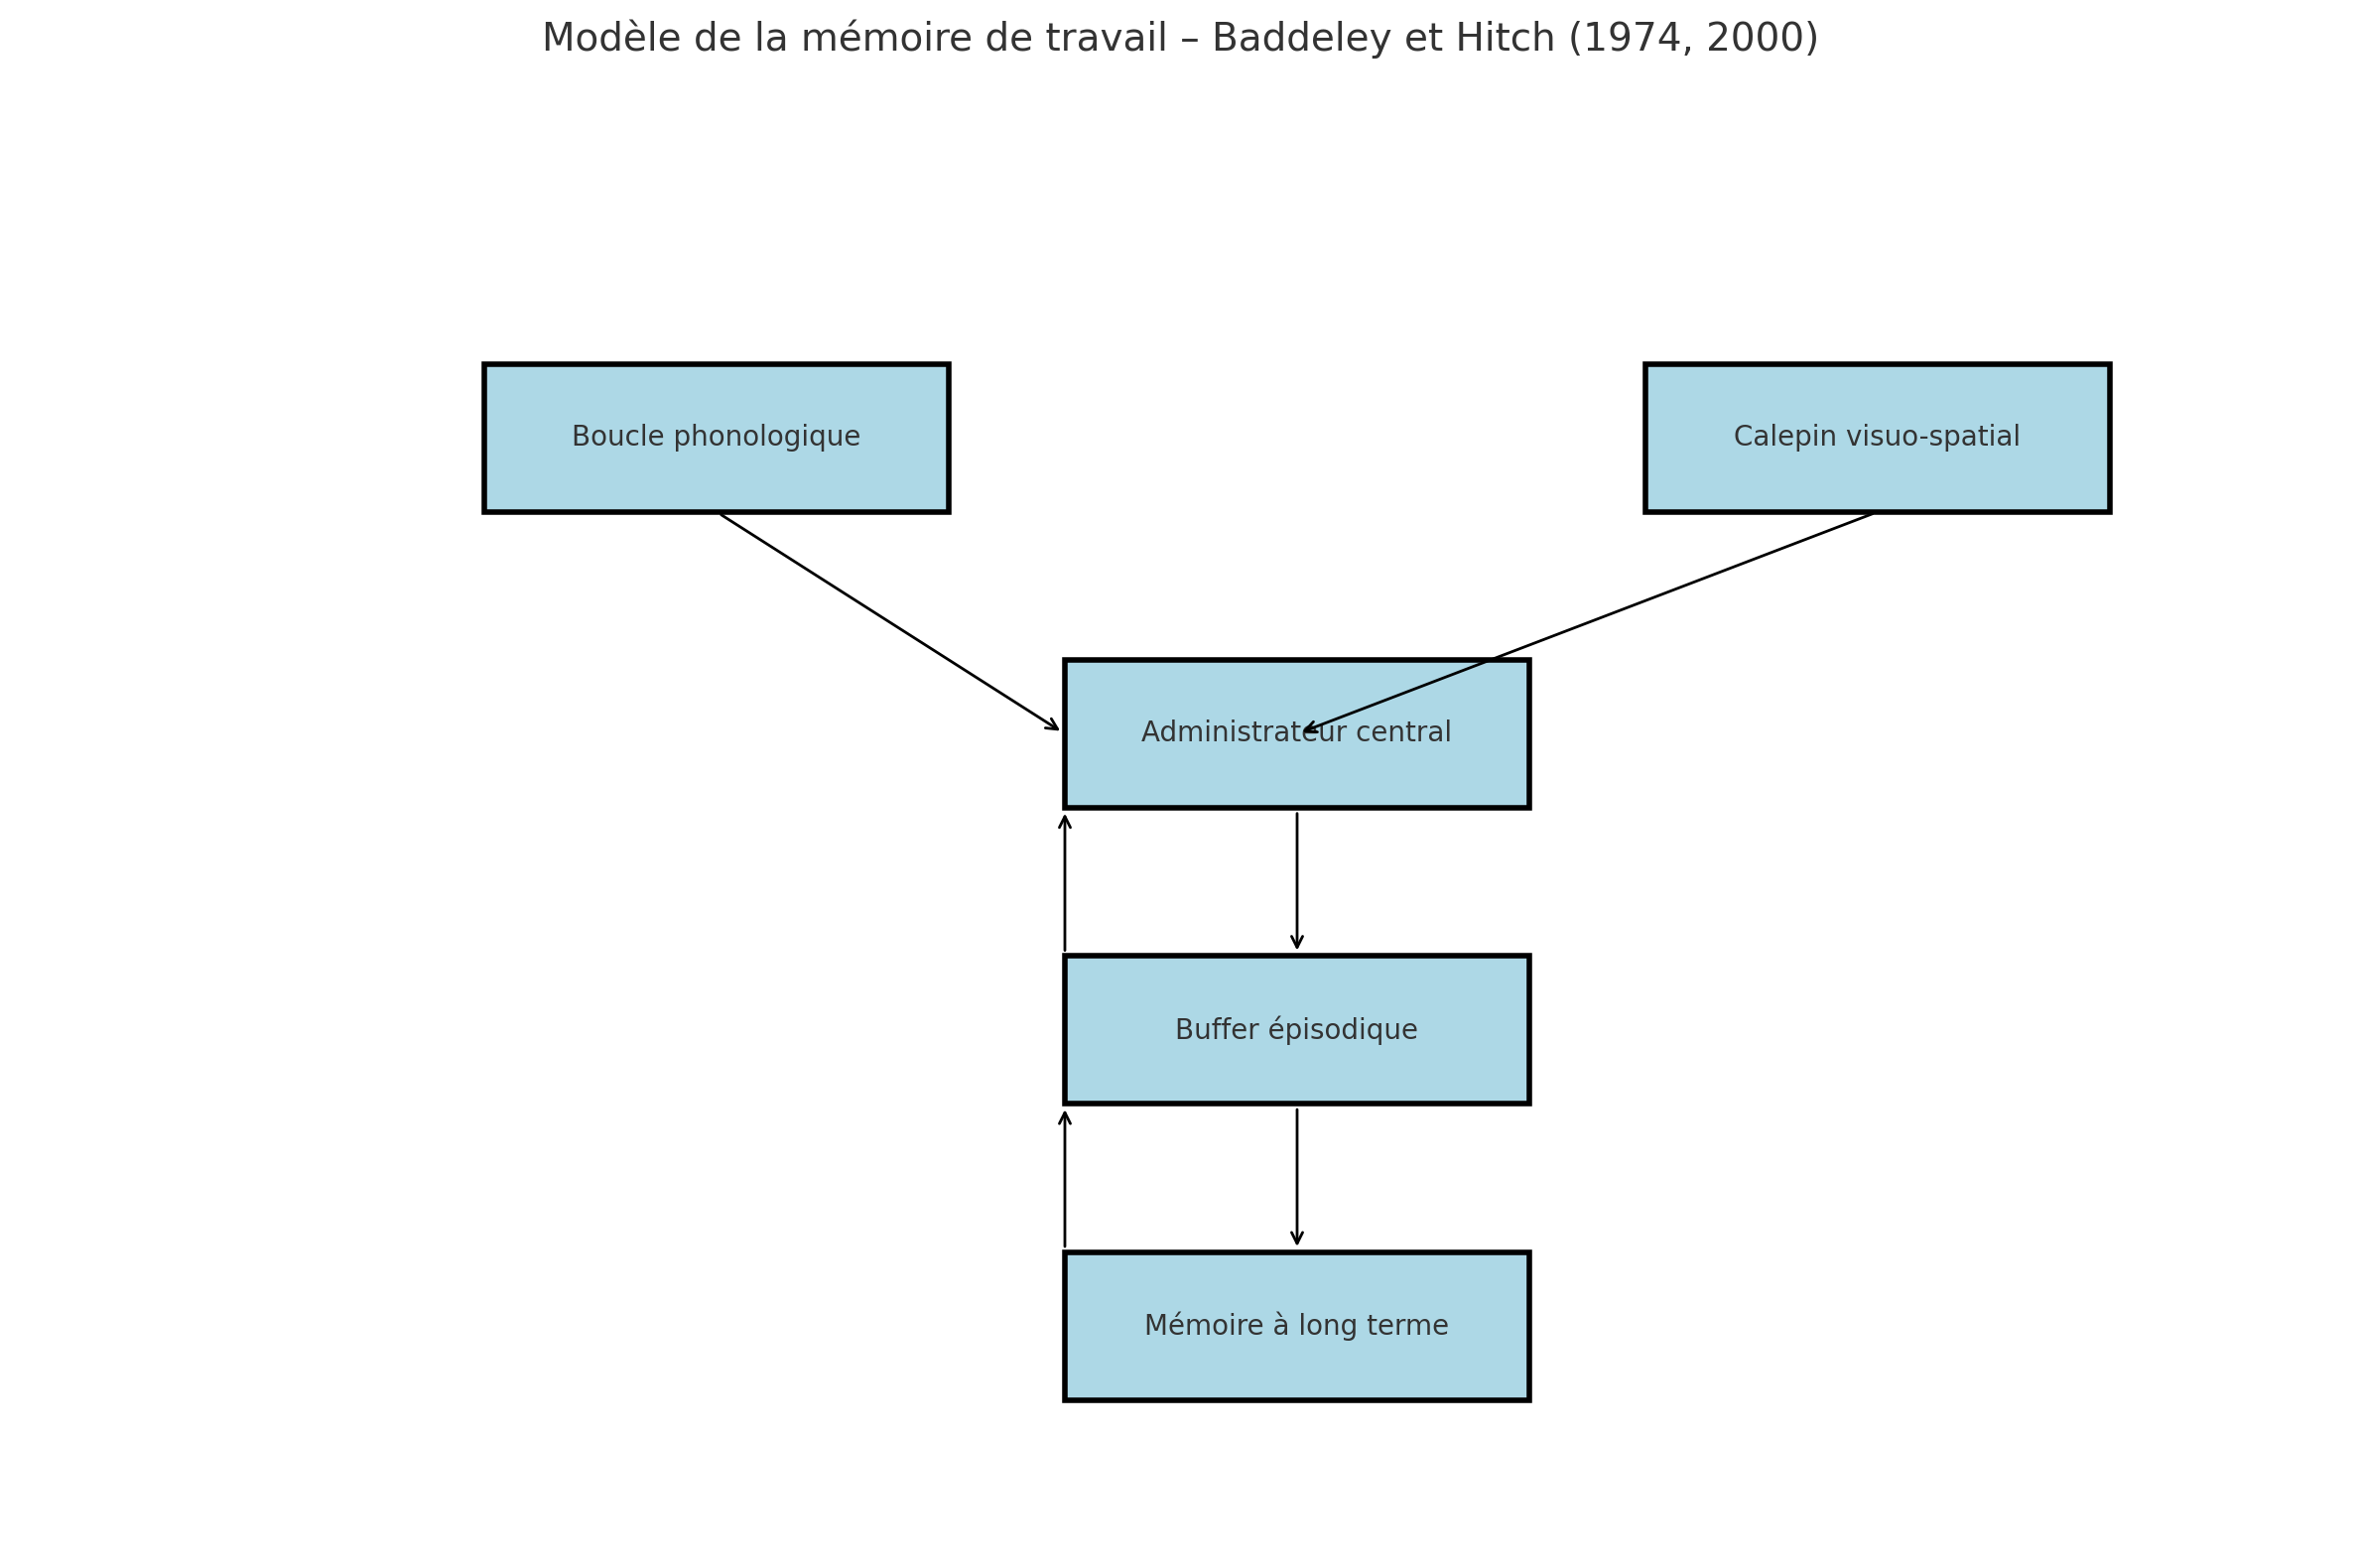
\includegraphics[width=0.7\textwidth]{images/1.1.1_2.png}
    \caption{schéma du modèle de la mémoire de travail de Baddeley et Hitch}
    \label{fig:beth}
\end{figure}

\begin{figure}[h]
    \centering
    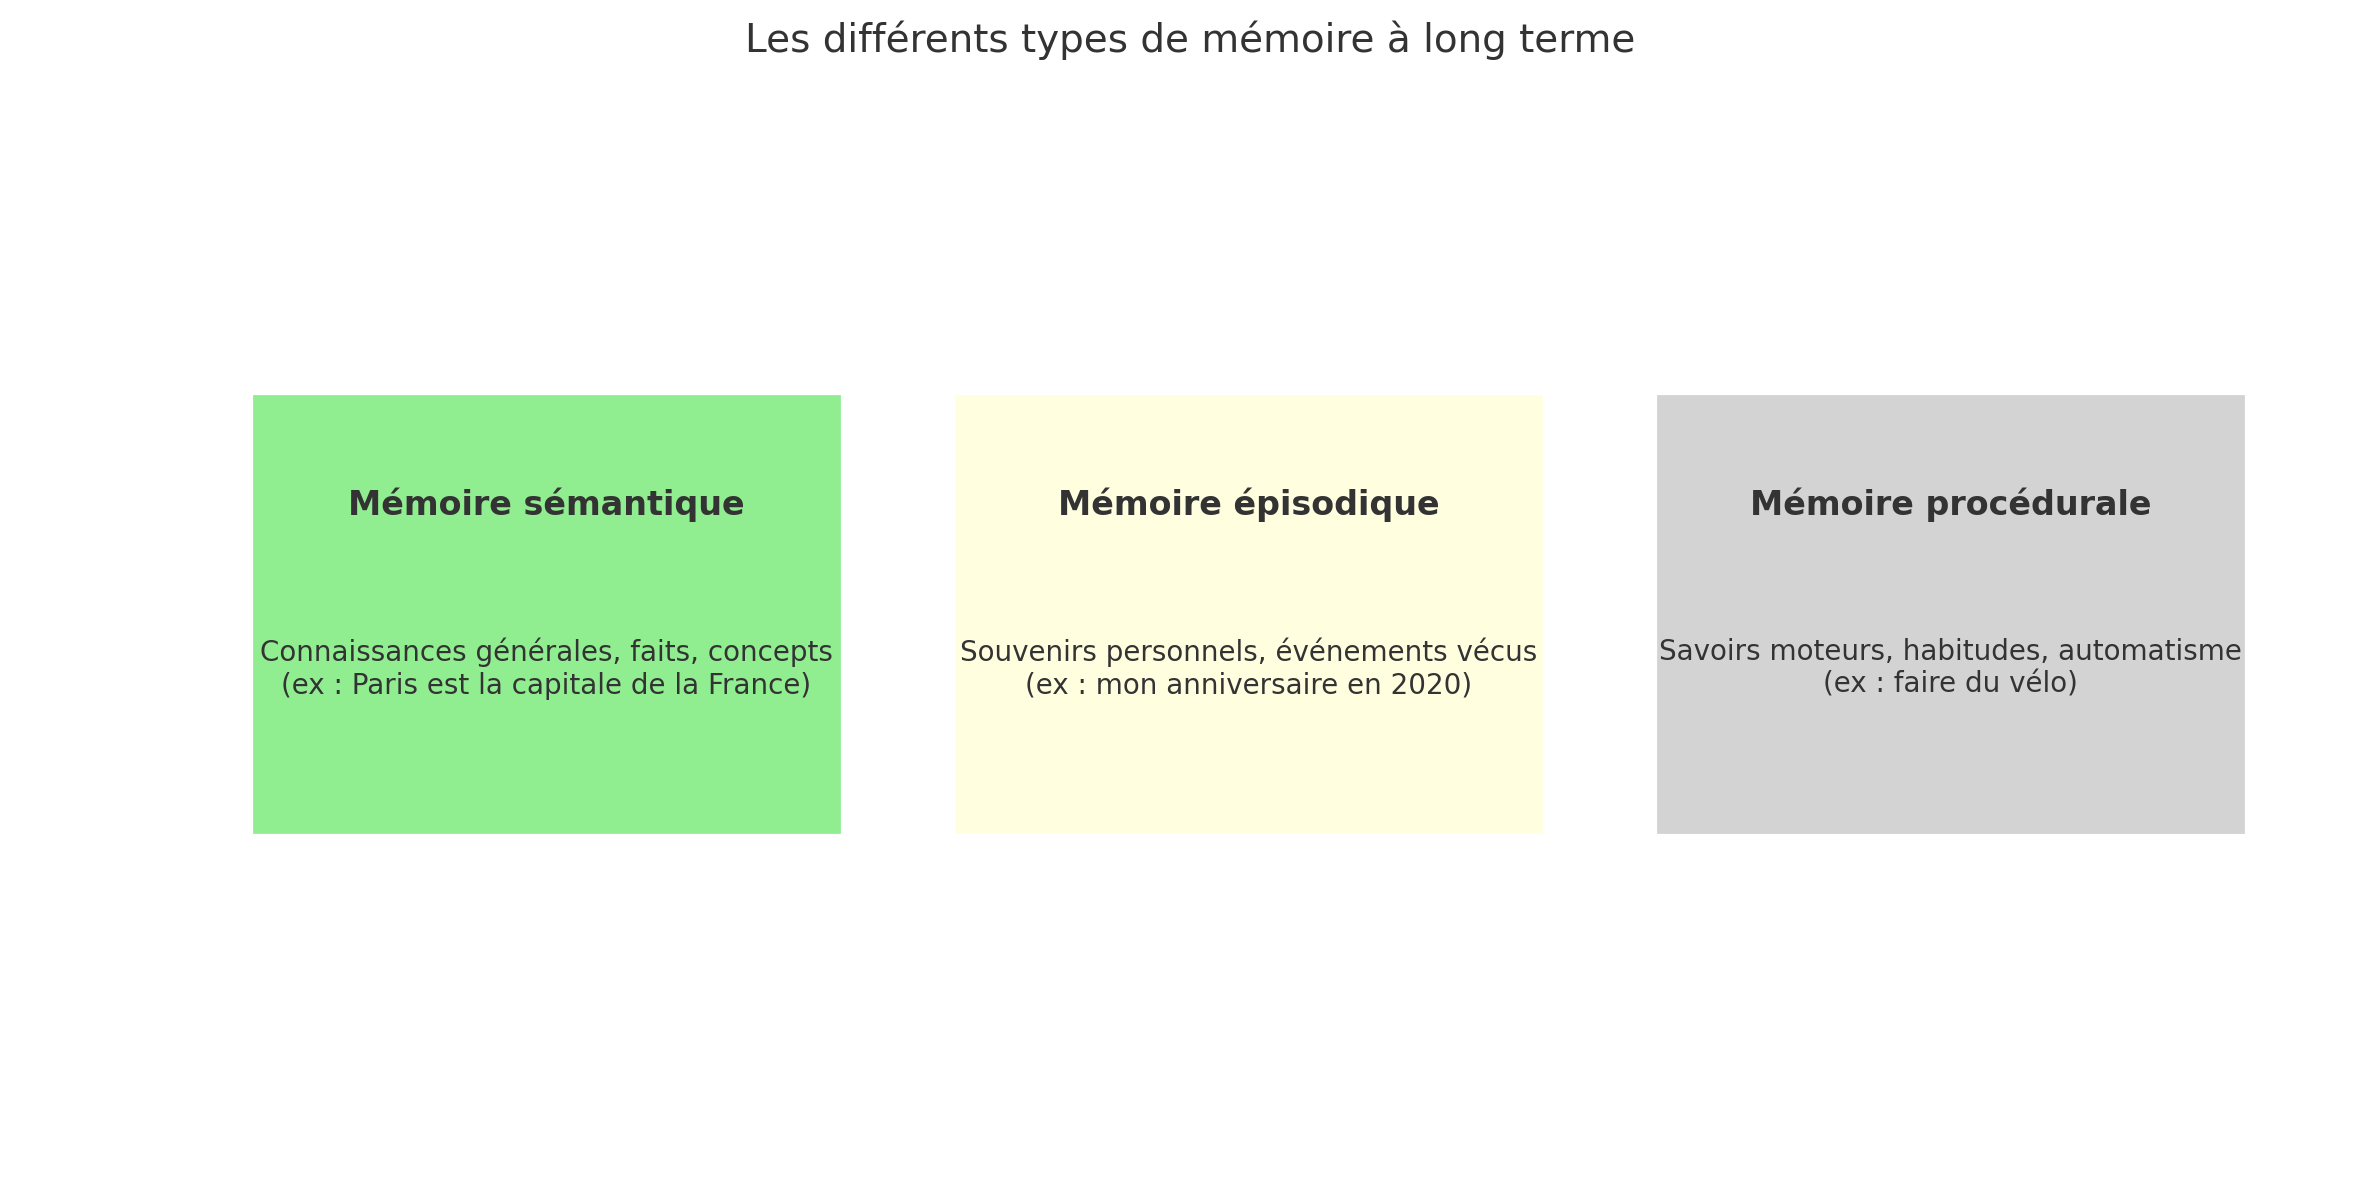
\includegraphics[width=0.7\textwidth]{images/1.1.2.png}
    \caption{Les différents types de mémoire à long terme}
    \label{fig:1.1.2}
\end{figure}

\end{document}
